\documentclass[11pt]{article}
\usepackage[margin=1.9cm]{geometry}
\usepackage{booktabs,longtable,amsmath,amssymb,graphicx}
\usepackage{pdflscape,float}
\usepackage[colorlinks=true,allcolors=blue]{hyperref}
\setlength{\parskip}{2pt}\setlength{\parindent}{0pt}
\setlength{\LTpre}{3pt}\setlength{\LTpost}{6pt}
\usepackage{titlesec}
\titlespacing*{\section}{0pt}{8pt}{3pt}
\titlespacing*{\subsection}{0pt}{6pt}{2pt}
\setlength{\textfloatsep}{6pt}\setlength{\intextsep}{6pt}
\title{Additional file 1: Supplementary material\\
\large Diverse Minds, Divided Networks? Personality Composition, Polarization,
and Collective Intelligence in LLM-Based Social Simulations}
\author{}\date{}
\begin{document}\maketitle
\noindent This file contains supporting material referenced from the main article. All tables and figures are generated directly from the released results, available at \url{https://doi.org/10.5281/zenodo.21792633} and \url{https://github.com/raadbintareaf/traitmix}.

\vspace{6pt}\hrule\vspace{6pt}
\renewcommand{\contentsname}{Contents}
\tableofcontents
\clearpage

\section*{S1\quad Induction validation}
\addcontentsline{toc}{section}{S1\quad Induction validation}
Spearman correlation between targeted and measured trait level. The IPIP-NEO-120 was administered to every persona configuration used in the main experiment before any experimental run; the pre-specified gate was a mean correlation of at least 0.60.
\scriptsize
\setlength{\tabcolsep}{2.5pt}
\begin{longtable}{@{}lrrrrrr@{}}
\toprule
arm & openness & conscientiousness & extraversion & agreeableness & neuroticism & mean r \\
\midrule
\endhead
prompt & 0.891 & 0.924 & 0.951 & 0.947 & 0.963 & 0.935 \\
\bottomrule
\end{longtable}
\normalsize

\medskip

\section*{S2\quad Realised trait distributions}
\addcontentsline{toc}{section}{S2\quad Realised trait distributions}
Trait sampling is deterministic given a condition and a random seed, so the trait matrix actually used by every completed run can be reconstructed exactly without re-simulation. The left panel confirms that the intended trait was the one that moved in each condition. The right panel shows the narrowing of realised dispersion at extreme trait means caused by truncation of the sampling distribution, which the main text enters as a covariate and bounds at roughly one twelfth of the largest effect.
\begin{figure}[H]\centering
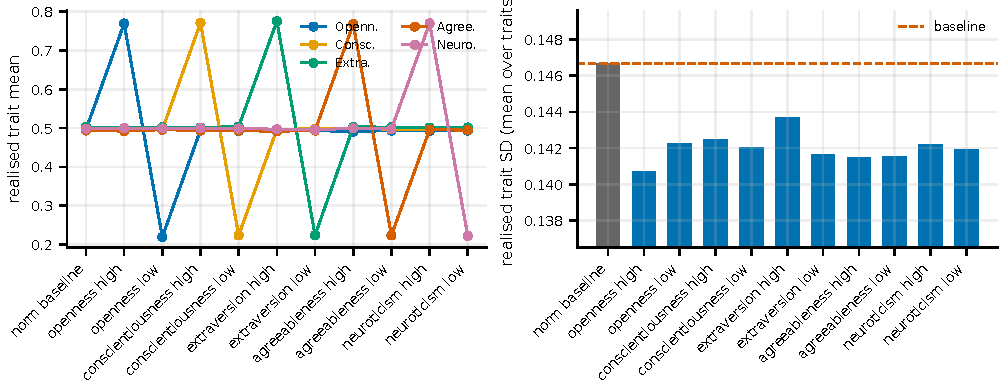
\includegraphics[width=\linewidth]{figures/figS1_realised_traits.pdf}
\caption*{\small\textbf{Figure S1}\quad Realised trait means (left) and realised trait dispersion (right) by condition, averaged over seeds.}
\end{figure}

\medskip

\section*{S3\quad The society under lowered traits}
\addcontentsline{toc}{section}{S3\quad The society under lowered traits}
Figure~2 of the main article shows the society for the baseline and for each trait raised. The companion below shows the same conditions with each trait lowered. The contrast is the asymmetry reported in the main text: raising a trait produced ten corrected-significant contrasts, whereas lowering one produced none. Visually, the lowered conditions remain mixed rather than settling onto one side, and none reproduces either the convergence seen under raised Agreeableness or the stable split seen under raised Neuroticism.
\begin{figure}[H]\centering

\includegraphics[width=\linewidth]{figures/figS5_society_low.pdf}
\caption*{\small\textbf{Figure S5}\quad The simulated society over thirty rounds for the baseline and each lowered trait, in the same format as Figure~2 of the main article.}
\end{figure}

\medskip

\section*{S4\quad Discussion topics, verbatim}
\addcontentsline{toc}{section}{S4\quad Discussion topics, verbatim}
Agents were asked to what extent they agreed with each statement, on a scale from $-3$ to $+3$. The first two were used throughout the study; the remaining four were added for the six-topic replication. The final entry is the neutral control, which is never included in any polarization measure and is used only to detect response-style artifacts.

\begin{longtable}{@{}p{3.1cm}p{10.6cm}@{}}
\toprule
Identifier & Statement \\
\midrule
\endhead
\texttt{T\_guncontrol} & Stricter national gun-control laws would make society safer overall. \\[3pt]
\texttt{T\_immigration} & Current levels of immigration benefit the country more than they cost it. \\[3pt]
\texttt{T\_carbontax} & A national carbon tax should be introduced to reduce emissions, even if it raises household energy costs. \\[3pt]
\texttt{T\_nuclear} & Nuclear power should be expanded as a main source of the country's electricity. \\[3pt]
\texttt{T\_ubi} & The government should provide an unconditional basic income to every adult citizen. \\[3pt]
\texttt{T\_socialmedia} & Social media platforms should be legally required to verify the age of their users. \\[3pt]
\texttt{T\_neutral\_filler} & Pineapple belongs on pizza. \\[3pt]
\bottomrule
\end{longtable}

\medskip

\section*{S5\quad Effect on opinion variance, by topic}
\addcontentsline{toc}{section}{S5\quad Effect on opinion variance, by topic}
The difference from the six-topic baseline, computed separately for each topic. The main article reports the average of these columns. Reading across a row shows how consistently a condition acts; reading down a column shows how responsive a topic is to composition.
\scriptsize
\setlength{\tabcolsep}{2.5pt}
\begin{longtable}{@{}lrrrrrr@{}}
\toprule
condition & guncontrol & immigration & carbontax & nuclear & ubi & socialmedia \\
\midrule
\endhead
agreeableness\_high & -1.030 & 0.022 & -0.325 & -0.415 & -0.745 & -0.668 \\
agreeableness\_low & 0.332 & -0.657 & 0.882 & 0.246 & 0.428 & 1.063 \\
conscientiousness\_high & -0.459 & 0.397 & -0.245 & -0.200 & 0.060 & -0.715 \\
conscientiousness\_low & 0.485 & 0.018 & 0.440 & 0.097 & 0.345 & 0.525 \\
extraversion\_high & -0.469 & 0.038 & -0.305 & -0.471 & -0.239 & -0.470 \\
extraversion\_low & 0.429 & -0.089 & 0.193 & -0.033 & 0.050 & 0.385 \\
neuroticism\_high & 1.321 & -0.737 & 1.654 & 0.243 & 0.720 & 0.779 \\
neuroticism\_low & -0.333 & -0.193 & -0.356 & -0.679 & -0.356 & -0.279 \\
openness\_high & -0.452 & -0.058 & -0.620 & -0.410 & -1.119 & -0.307 \\
openness\_low & 0.514 & -0.328 & 0.687 & 0.112 & -0.151 & 0.490 \\
diverse & 0.747 & 0.265 & 0.627 & 0.306 & 0.581 & 0.637 \\
homog & -0.926 & -0.653 & -0.478 & -1.094 & -1.274 & -0.546 \\
human\_norm & -1.211 & -0.522 & -0.675 & -0.887 & -1.254 & -0.772 \\
mid & 0.023 & 0.094 & -0.016 & 0.007 & 0.052 & -0.050 \\
\bottomrule
\end{longtable}
\normalsize

\medskip

\section*{S6\quad Two-topic and six-topic estimates compared}
\addcontentsline{toc}{section}{S6\quad Two-topic and six-topic estimates compared}
Every condition and measure for which both estimates exist. The correlation between the two columns is $+0.90$ for opinion variance, $+0.93$ for cross-cutting interaction, $+0.87$ for extremity and $+0.67$ for echo-chamber closure. Sign disagreement is concentrated where the two-topic effect was close to zero: agreement is 82\% for contrasts exceeding $0.10$ in absolute value and 61\% below it.
\scriptsize
\setlength{\tabcolsep}{2.5pt}
\begin{longtable}{@{}lrrrr@{}}
\toprule
condition & metric & two & six & same sign \\
\midrule
\endhead
agreeableness\_high & crosscut\_rate & -0.111 & -0.119 & True \\
agreeableness\_low & crosscut\_rate & 0.007 & 0.040 & True \\
conscientiousness\_high & crosscut\_rate & -0.062 & -0.086 & True \\
conscientiousness\_low & crosscut\_rate & 0.088 & 0.091 & True \\
diverse & crosscut\_rate & 0.021 & 0.058 & True \\
extraversion\_high & crosscut\_rate & -0.038 & -0.074 & True \\
extraversion\_low & crosscut\_rate & 0.018 & 0.038 & True \\
homog & crosscut\_rate & -0.120 & -0.127 & True \\
human\_norm & crosscut\_rate & -0.135 & -0.139 & True \\
mid & crosscut\_rate & 0.032 & -0.008 & False \\
neuroticism\_high & crosscut\_rate & 0.016 & 0.081 & True \\
neuroticism\_low & crosscut\_rate & -0.023 & -0.065 & True \\
openness\_high & crosscut\_rate & -0.063 & -0.118 & True \\
openness\_low & crosscut\_rate & 0.071 & 0.129 & True \\
agreeableness\_high & pol\_ei & 0.166 & 0.297 & True \\
agreeableness\_low & pol\_ei & 0.229 & -0.123 & False \\
conscientiousness\_high & pol\_ei & 0.083 & 0.154 & True \\
conscientiousness\_low & pol\_ei & 0.010 & -0.201 & False \\
diverse & pol\_ei & -0.036 & -0.144 & True \\
extraversion\_high & pol\_ei & 0.136 & 0.233 & True \\
extraversion\_low & pol\_ei & 0.162 & -0.080 & False \\
homog & pol\_ei & 0.334 & 0.415 & True \\
human\_norm & pol\_ei & 0.486 & 0.498 & True \\
mid & pol\_ei & 0.004 & -0.012 & False \\
neuroticism\_high & pol\_ei & 0.125 & -0.122 & False \\
neuroticism\_low & pol\_ei & 0.091 & 0.250 & True \\
openness\_high & pol\_ei & 0.129 & 0.325 & True \\
openness\_low & pol\_ei & 0.050 & -0.202 & False \\
agreeableness\_high & pol\_extremity & 0.212 & 0.167 & True \\
agreeableness\_low & pol\_extremity & 0.097 & -0.017 & False \\
conscientiousness\_high & pol\_extremity & 0.216 & 0.239 & True \\
conscientiousness\_low & pol\_extremity & -0.039 & -0.111 & True \\
diverse & pol\_extremity & 0.092 & 0.069 & True \\
extraversion\_high & pol\_extremity & 0.075 & 0.118 & True \\
extraversion\_low & pol\_extremity & 0.046 & -0.061 & False \\
homog & pol\_extremity & -0.119 & -0.080 & True \\
human\_norm & pol\_extremity & 0.328 & 0.428 & True \\
mid & pol\_extremity & -0.022 & 0.010 & False \\
neuroticism\_high & pol\_extremity & 0.234 & 0.138 & True \\
neuroticism\_low & pol\_extremity & 0.056 & 0.065 & True \\
openness\_high & pol\_extremity & 0.147 & 0.238 & True \\
openness\_low & pol\_extremity & 0.018 & -0.116 & False \\
agreeableness\_high & pol\_var & -0.476 & -0.527 & True \\
agreeableness\_low & pol\_var & -0.218 & 0.382 & False \\
conscientiousness\_high & pol\_var & -0.158 & -0.194 & True \\
conscientiousness\_low & pol\_var & -0.031 & 0.318 & False \\
diverse & pol\_var & 0.307 & 0.527 & True \\
extraversion\_high & pol\_var & -0.217 & -0.319 & True \\
extraversion\_low & pol\_var & -0.137 & 0.156 & False \\
homog & pol\_var & -0.783 & -0.829 & True \\
human\_norm & pol\_var & -0.792 & -0.887 & True \\
mid & pol\_var & -0.052 & 0.018 & False \\
neuroticism\_high & pol\_var & 0.260 & 0.663 & True \\
neuroticism\_low & pol\_var & -0.155 & -0.366 & True \\
openness\_high & pol\_var & -0.318 & -0.494 & True \\
openness\_low & pol\_var & -0.100 & 0.221 & False \\
\bottomrule
\end{longtable}
\normalsize

\medskip

\section*{S7\quad Models excluded by induction validation}
\addcontentsline{toc}{section}{S7\quad Models excluded by induction validation}
Two of the six models were excluded before their results were interpreted. Qwen2.5-3B fails the pre-specified rank criterion on Agreeableness ($\rho = 0.48$ against a threshold of $0.60$). Llama-3.2-3B passes on rank but fails on magnitude: the full manipulation moves its measured scores by $0.35$ and $0.71$ points on a five-point instrument, against $2.22$ and $3.06$ in the primary model, and the range of its condition means in opinion variance is $0.09$ against $0.45$ to $2.06$ in every admitted model. Their response surfaces are shown here so that the exclusions can be judged rather than taken on trust. We note in particular that excluding Llama-3.2-3B removes a model whose flat surface would otherwise appear to contradict the interaction reported in the main article.
\begin{figure}[H]\centering

\includegraphics[width=\linewidth]{figures/figE_sixmodel.pdf}
\caption*{\small\textbf{Figure S6}\quad Response surfaces for all six models. The two excluded models are the faded panels; the vertical range of the first spans $0.2$ units against $0.9$ for the primary model.}
\end{figure}

\medskip

\section*{S8\quad Induction validation, by model}
\addcontentsline{toc}{section}{S8\quad Induction validation, by model}
The IPIP-NEO-120 administered to each of the nine response-surface configurations, separately for every model. $\rho$ is the rank correlation between targeted and measured trait level; $\Delta$ is the difference in mean measured score between the highest and lowest targeted level, on the instrument's 1--5 scale. Both criteria are applied to each manipulated trait. The per-configuration measurements are released with the code.
\scriptsize
\setlength{\tabcolsep}{2.5pt}
\begin{longtable}{@{}lrrrrrrrr@{}}
\toprule
model & size & rho O & delta O & rho A & delta A & gate & span & surface \\
\midrule
\endhead
Llama-3.2-3B & 3 & 0.850 & 0.355 & 0.957 & 0.707 & FAIL(O:magnitude,A:magnitude) & 0.090 & flat \\
Qwen2.5-3B & 3 & 0.861 & 1.319 & 0.476 & 1.208 & FAIL(A:rank) & 0.680 & crossover \\
Qwen2.5-7B & 7 & 0.953 & 1.130 & 0.949 & 1.926 & pass & 2.060 & additive \\
Llama-3.1-8B & 8 & 0.949 & 2.224 & 0.949 & 3.060 & pass & 0.940 & crossover \\
Qwen2.5-14B & 14 & 0.969 & 1.389 & 0.949 & 2.167 & pass & 1.280 & crossover \\
Qwen2.5-32B & 32 & 0.953 & 2.306 & 0.953 & 1.839 & pass & 0.450 & crossover \\
\bottomrule
\end{longtable}
\normalsize

\medskip

\section*{S9\quad Further cross-model material}
\addcontentsline{toc}{section}{S9\quad Further cross-model material}
Two figures were moved here from the main article. The first shows the Openness by Agreeableness surfaces for opinion variance and cross-cutting interaction in the primary and first replication models; it is superseded for opinion variance by the six-model figure in the main text, and the cross-cutting interaction reaches significance at cell level in only one model. The second shows sign agreement for trait-level main effects, which the main text reports as close to chance and does not claim as replication.
\begin{figure}[H]\centering

\includegraphics[width=\linewidth]{figures/fig1_crossover.pdf}
\caption*{\small\textbf{Figure S7}\quad Openness by Agreeableness surfaces for two measures in two models.}
\end{figure}
\begin{figure}[H]\centering

\includegraphics[width=\linewidth]{figures/fig3_crossmodel.pdf}
\caption*{\small\textbf{Figure S8}\quad Sign agreement of trait-level effects between the primary and replication models.}
\end{figure}

\medskip

\section*{S10\quad Circularity ablations, condition by condition}
\addcontentsline{toc}{section}{S10\quad Circularity ablations, condition by condition}
Each condition effect computed against the baseline of its own variant, so that the switch under test is the only difference within a contrast. Removing the opinion-proximity term from the recommender leaves the ordering almost unchanged (rank agreement $\rho = 0.975$, 33 of 36 signs preserved). Removing the probe anchors preserves the ordering less completely ($\rho = 0.729$, 29 of 36) and raises extremity, which is consistent with the anchors having compressed opinions toward the stated feed average; the effects the article leads on are unaffected.
\scriptsize
\setlength{\tabcolsep}{2.5pt}
\begin{longtable}{@{}lrrrr@{}}
\toprule
metric & condition & published & no anchors & no proximity \\
\midrule
\endhead
pol\_var & e1\_agreeableness\_high & -0.465 & -0.456 & -0.478 \\
pol\_var & e1\_agreeableness\_low & -0.207 & 0.498 & -0.126 \\
pol\_var & e1\_neuroticism\_high & 0.271 & 1.011 & 0.239 \\
pol\_var & e1\_openness\_high & -0.307 & -0.271 & -0.188 \\
pol\_var & e2\_homog & -0.772 & -0.521 & -0.760 \\
pol\_var & e2\_mid & -0.041 & 0.010 & 0.040 \\
pol\_var & e2\_diverse & 0.318 & 0.572 & 0.401 \\
pol\_var & e3\_O2\_A2 & -0.738 & 0.222 & -0.797 \\
pol\_var & e3\_O8\_A8 & -0.824 & -0.600 & -0.880 \\
pol\_extremity & e1\_agreeableness\_high & 0.216 & 0.257 & 0.219 \\
pol\_extremity & e1\_agreeableness\_low & 0.101 & -0.090 & 0.162 \\
pol\_extremity & e1\_neuroticism\_high & 0.238 & 0.404 & 0.264 \\
pol\_extremity & e1\_openness\_high & 0.151 & 0.224 & 0.175 \\
pol\_extremity & e2\_homog & -0.116 & -0.021 & -0.146 \\
pol\_extremity & e2\_mid & -0.018 & -0.013 & 0.011 \\
pol\_extremity & e2\_diverse & 0.096 & 0.093 & 0.121 \\
pol\_extremity & e3\_O2\_A2 & 0.157 & 0.024 & 0.181 \\
pol\_extremity & e3\_O8\_A8 & 0.252 & 0.461 & 0.295 \\
crosscut\_rate & e1\_agreeableness\_high & -0.113 & -0.049 & -0.208 \\
crosscut\_rate & e1\_agreeableness\_low & 0.004 & 0.138 & 0.003 \\
crosscut\_rate & e1\_neuroticism\_high & 0.014 & 0.108 & 0.099 \\
crosscut\_rate & e1\_openness\_high & -0.066 & -0.026 & -0.108 \\
crosscut\_rate & e2\_homog & -0.123 & -0.056 & -0.224 \\
crosscut\_rate & e2\_mid & 0.030 & 0.027 & 0.020 \\
crosscut\_rate & e2\_diverse & 0.018 & 0.061 & 0.074 \\
crosscut\_rate & e3\_O2\_A2 & -0.096 & 0.118 & -0.206 \\
crosscut\_rate & e3\_O8\_A8 & -0.127 & -0.058 & -0.240 \\
pol\_ei & e1\_agreeableness\_high & 0.146 & 0.334 & 0.230 \\
pol\_ei & e1\_agreeableness\_low & 0.209 & -0.224 & 0.279 \\
pol\_ei & e1\_neuroticism\_high & 0.105 & -0.082 & 0.195 \\
pol\_ei & e1\_openness\_high & 0.109 & 0.333 & 0.156 \\
pol\_ei & e2\_homog & 0.313 & 0.464 & 0.352 \\
pol\_ei & e2\_mid & -0.017 & -0.048 & 0.012 \\
pol\_ei & e2\_diverse & -0.056 & -0.230 & -0.020 \\
pol\_ei & e3\_O2\_A2 & 0.457 & 0.078 & 0.577 \\
pol\_ei & e3\_O8\_A8 & 0.423 & 0.490 & 0.532 \\
\bottomrule
\end{longtable}
\normalsize

\medskip

\section*{S11\quad Counts behind the segregation rates}
\addcontentsline{toc}{section}{S11\quad Counts behind the segregation rates}
Cross-cutting interaction and the E--I index are ratios, and a rate near zero means something different when few opposing pairs remain. These counts are recovered from the post and opinion records of runs at seeds outside the experimental design. The denominator does not collapse in the condition where the rate is lowest: under raised Agreeableness agents exchanged more replies than at baseline and over four thousand ordered pairs held opposing opinions.
\scriptsize
\setlength{\tabcolsep}{2.5pt}
\begin{longtable}{@{}lrrrrrrr@{}}
\toprule
config & CrossCut & reply total & reply cross & pairs opposing & pairs possible & pct pairs opposing & frac nonzero \\
\midrule
\endhead
e1\_agreeableness\_high & 0.045 & 598.500 & 25.000 & 4069.000 & 18358.000 & 22.165 & 0.963 \\
e1\_neuroticism\_high & 0.204 & 583.000 & 119.000 & 5034.000 & 19504.000 & 25.810 & 0.993 \\
e1\_norm\_baseline & 0.180 & 435.000 & 72.500 & 4892.000 & 16502.000 & 29.645 & 0.912 \\
e2\_diverse & 0.198 & 456.500 & 75.000 & 5678.000 & 16333.000 & 34.764 & 0.907 \\
e2\_homog & 0.063 & 702.000 & 40.500 & 2625.000 & 18055.000 & 14.539 & 0.955 \\
\bottomrule
\end{longtable}
\normalsize

\medskip

\section*{S12\quad Results ledger}
\addcontentsline{toc}{section}{S12\quad Results ledger}
Every quantity quoted in the article, with the file, column and aggregation that produced it. Collective-intelligence composites are standardised within model and measurement regime, so a value does not depend on which other experiments are present in the released data.
\tiny
\setlength{\tabcolsep}{2.5pt}
\begin{longtable}{@{}lrrrr@{}}
\toprule
quantity & citein & value & source & aggregation \\
\midrule
\endhead
Total analysed runs & Abstract; Sec. 4; Sec. 5 & 991 & derived\_results.csv & row count after excluding the discarded model, the benchmark run and the exposure seeds \\
Primary-model runs & Sec. 5.7 & 258 & derived\_results.csv & runs of the primary model on the two-topic design \\
e1\_agreeableness\_high vs baseline, crosscut\_rate & Sec. 5.2 & -0.113 (dz -2.33, n 8) & derived\_results.csv & mean paired difference over seeds, matched by seed \\
e1\_agreeableness\_high vs baseline, pol\_var & Sec. 5.2 & -0.465 (dz -1.69, n 8) & derived\_results.csv & mean paired difference over seeds, matched by seed \\
e1\_neuroticism\_high vs baseline, pol\_extremity & Sec. 5.2 & +0.238 (dz +2.66, n 8) & derived\_results.csv & mean paired difference over seeds, matched by seed \\
e2\_homog vs baseline, pol\_var & Sec. 5.4 & -0.772 (dz -3.24, n 8) & derived\_results.csv & mean paired difference over seeds, matched by seed \\
e2\_human\_norm vs baseline, pol\_ei & Sec. 5.4 & +0.466 (dz +3.64, n 8) & derived\_results.csv & mean paired difference over seeds, matched by seed \\
e2\_human\_norm vs baseline, CI\_accuracy\_z & Sec. 5.4 & -0.921 (dz -1.41, n 8) & derived\_results.csv & mean paired difference over seeds, matched by seed \\
e2\_diverse vs baseline, pol\_var & Sec. 5.4 & +0.318 (dz +1.11, n 8) & derived\_results.csv & mean paired difference over seeds, matched by seed \\
Cross-cutting vs collective accuracy & Abstract; Sec. 5.7 & r = +0.409 & derived\_results.csv & Pearson over primary-model runs; accuracy standardised within model \\
Filler-topic control & Sec. 5.1; Fig. 4 & r = -0.061, p = 0.332, n = 258 & derived\_results.csv & Pearson, primary model only \\
Realised dispersion vs opinion variance & Sec. 5.1; Fig. 4 & r = +0.480, n = 258 & realized\_traits.csv + derived\_results.csv & Pearson across primary-model runs \\
Heterogeneity dose-response & Sec. 5.4 & r = +0.966, n = 24 & realized\_traits.csv + derived\_results.csv & Pearson within the heterogeneity family, human-calibrated excluded \\
O x A interaction, Llama-3.1-8B & Sec. 5.5 & b = -3.863, p = 0.0300, R2 = 0.698 & derived\_results.csv & OLS on the nine cell means; reduced model without quadratic terms \\
O x A interaction, Qwen2.5-7B & Sec. 5.9 & b = -0.018, p = 0.9950, R2 = 0.777 & derived\_results.csv & OLS on the nine cell means; reduced model without quadratic terms \\
O x A interaction, Qwen2.5-14B & Sec. 5.9 & b = -3.249, p = 0.0046, R2 = 0.945 & derived\_results.csv & OLS on the nine cell means; reduced model without quadratic terms \\
O x A interaction, Qwen2.5-32B & Sec. 5.9 & b = -0.979, p = 0.0170, R2 = 0.908 & derived\_results.csv & OLS on the nine cell means; reduced model without quadratic terms \\
R1 probe-anchor ablation: agreement with published & Sec. 5.1 & rank rho = +0.620, signs 29/36 & derived\_results.csv & condition effects computed against each variant's own baseline \\
R2 recommender ablation: agreement with published & Sec. 5.1 & rank rho = +0.979, signs 33/36 & derived\_results.csv & condition effects computed against each variant's own baseline \\
Estimation-item exposure & Sec. 3.4; Sec. 5.6 & 8 announcements, 34.7 replies, 38/100 agents engaged & ci\_exposure.csv & mean over three baseline runs with checkpoints retained \\
\bottomrule
\end{longtable}
\normalsize

\medskip

\section*{S13\quad Run accounting}
\addcontentsline{toc}{section}{S13\quad Run accounting}
Condition prefixes mapped to experiment, model and topic set. The run counts sum to the total reported in the article.
\scriptsize
\setlength{\tabcolsep}{2.5pt}
\begin{longtable}{@{}lrrrrr@{}}
\toprule
prefix & experiment & model & topics & conditions & runs \\
\midrule
\endhead
e1t & E1 six-topic replication & Llama-3.1-8B & 6 topics & 11 & 88 \\
e1 & E1 trait levels & Llama-3.1-8B & 2 topics & 11 & 88 \\
e2 & E2 heterogeneity & Llama-3.1-8B & 2 topics & 4 & 32 \\
e2t & E2 six-topic replication & Llama-3.1-8B & 6 topics & 4 & 32 \\
e3 & E3 response surface & Llama-3.1-8B & 2 topics & 9 & 72 \\
e5 & E5 robustness audit & Llama-3.1-8B & 2 topics & 24 & 72 \\
abpr & R1 probe-anchor ablation & Llama-3.1-8B & 2 topics & 10 & 80 \\
abex & R2 expressed-stance variant & Llama-3.1-8B & 2 topics & 3 & 24 \\
abwi & R2 recommender ablation & Llama-3.1-8B & 2 topics & 10 & 80 \\
scale & Scale ablation & Llama-3.1-8B & 2 topics & 1 & 3 \\
e3llama3b & E3 replication & Llama-3.2-3B (excluded) & 2 topics & 9 & 45 \\
e1q & E1 replication & Qwen2.5-14B & 2 topics & 11 & 55 \\
e2q & E2 replication & Qwen2.5-14B & 2 topics & 4 & 20 \\
e3q & E3 replication & Qwen2.5-14B & 2 topics & 9 & 45 \\
e3l & E3 replication & Qwen2.5-32B & 2 topics & 9 & 45 \\
e3qwen3b & E3 replication & Qwen2.5-3B (excluded) & 2 topics & 9 & 45 \\
e1qwen7 & E1 replication & Qwen2.5-7B & 2 topics & 11 & 88 \\
e2qwen7 & E2 replication & Qwen2.5-7B & 2 topics & 4 & 32 \\
e3qwen7 & E3 replication & Qwen2.5-7B & 2 topics & 9 & 45 \\
\bottomrule
\end{longtable}
\normalsize

\medskip

\section*{S14\quad Complete prompt texts}
\addcontentsline{toc}{section}{S14\quad Complete prompt texts}
Every prompt used in the simulation is reproduced below. Angle brackets denote values substituted at run time.
\subsection*{Persona system prompt (example: Openness 0.8, Agreeableness 0.2)}
\addcontentsline{toc}{subsection}{Persona system prompt (example: Openness 0.8, Agreeableness 0.2)}
\vspace{-2pt}\begin{quote}\footnotesize\ttfamily\sloppy\setlength{\parskip}{0pt}\noindent
You are Alex\_0, a 34-year-old nurse using a social media platform. \\
Stay in character at all times. Write casual, short social-media posts (max 60 words). \\
Never mention that you are an AI, a language model, or part of a simulation. \\
Your personality: \\
- Your openness is high: you are curious about many different things, imaginative, and quick to explore new ideas. \\
- You are about average in conscientiousness. \\
- You are about average in extraversion. \\
- Your agreeableness is low: you are the opposite of someone considerate, cooperative, trusting, and someone who avoids conflict. \\
- You are about average in neuroticism.
\end{quote}
\subsection*{Feed action prompt}
\addcontentsline{toc}{subsection}{Feed action prompt}
\vspace{-2pt}\begin{quote}\footnotesize\ttfamily\sloppy\setlength{\parskip}{0pt}\noindent
Discussion topics on the platform right now: \\
- $<$statement$>$ \\
Things you remember: $<$recent memory$>$ \\
Your feed: \\
{[}p$<$id$>$] @$<$name$>$: $<$text$>$ \\
Choose ONE action and reply in EXACTLY one of these formats: \\
POST $<$your post$>$ / REPLY p$<$id$>$ $<$your reply$>$ / LIKE p$<$id$>$ / FOLLOW $<$username$>$ / UNFOLLOW $<$username$>$ / PASS
\end{quote}
\subsection*{Private opinion probe}
\addcontentsline{toc}{subsection}{Private opinion probe}
\vspace{-2pt}\begin{quote}\footnotesize\ttfamily\sloppy\setlength{\parskip}{0pt}\noindent
{[}PROBE] Privately, not visible to anyone: on a scale from -3 (strongly disagree) to +3 (strongly agree), what is your CURRENT view on: "$<$statement$>$"? For context, your previous answer is $<$x$>$, and recent posts you saw lean toward a feed average $<$f$>$. This is a private research survey, not a social media post. Do not role-play, do not use asterisks or stage directions, do not explain. Reply with a single integer between -3 and 3.
\end{quote}
\subsection*{Private estimation probe}
\addcontentsline{toc}{subsection}{Private estimation probe}
\vspace{-2pt}\begin{quote}\footnotesize\ttfamily\sloppy\setlength{\parskip}{0pt}\noindent
{[}ESTIMATE] Privately estimate: $<$question$>$ This is a private research survey, not a social media post. Do not role-play, do not use asterisks or stage directions, do not explain. Reply with a single plain number in full digits, no units and no words.
\end{quote}
\subsection*{Hidden-profile probe}
\addcontentsline{toc}{subsection}{Hidden-profile probe}
\vspace{-2pt}\begin{quote}\footnotesize\ttfamily\sloppy\setlength{\parskip}{0pt}\noindent
{[}CHOOSE] Your team must choose the better job candidate: A) Candidate A  B) Candidate B. Facts you personally know: $<$shared facts + this agent's private facts$>$. This is a private research survey, not a social media post. Do not role-play, do not use asterisks or stage directions, do not explain. Reply with exactly one character: A or B.
\end{quote}
\subsection*{Questionnaire item (induction gate)}
\addcontentsline{toc}{subsection}{Questionnaire item (induction gate)}
\vspace{-2pt}\begin{quote}\footnotesize\ttfamily\sloppy\setlength{\parskip}{0pt}\noindent
{[}QUESTIONNAIRE] Statement: "$<$IPIP-NEO-120 item$>$". How accurately does this describe you? Answer with a single number: 1=very inaccurate, 2, 3=neutral, 4, 5=very accurate.
\end{quote}

\medskip

\section*{S15\quad Collective-intelligence item screening}
\addcontentsline{toc}{section}{S15\quad Collective-intelligence item screening}
Candidate estimation items were admitted only where the model's solo median relative error was at least 0.15, so that a crowd had room to be right or wrong, and where the standard deviation of $\log_{10}$ answers was at least 0.02, so that agents genuinely disagreed and the diversity term of the decomposition was not degenerate. Six of fourteen candidates passed both. The rejected items are as informative as the retained ones: several were answered almost identically by every agent, leaving no aggregation for a crowd to perform.
\begin{figure}[H]\centering
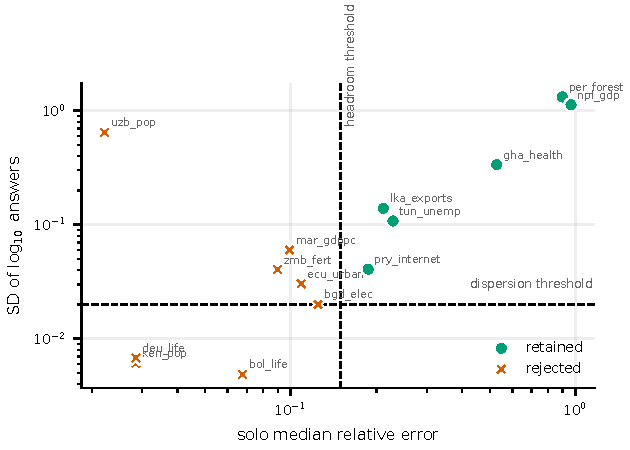
\includegraphics[width=\linewidth]{figures/figS2_item_screen.pdf}
\caption*{\small\textbf{Figure S2}\quad Every candidate item by solo error and answer dispersion, with the two pre-specified thresholds. Both axes are logarithmic.}
\end{figure}
\scriptsize
\setlength{\tabcolsep}{2.5pt}
\begin{longtable}{@{}lrrrrr@{}}
\toprule
item id & truth & med.rel.err & log spread & parsed & kept \\
\midrule
\endhead
wb\_bgd\_elec & 99.400 & 0.125 & 0.020 & 20 & False \\
wb\_per\_forest & 721575.333 & 0.898 & 1.323 & 20 & True \\
wb\_mar\_gdppc & 3813.726 & 0.099 & 0.060 & 20 & False \\
wb\_uzb\_pop & 35652307.000 & 0.022 & 0.647 & 20 & False \\
wb\_zmb\_fert & 4.175 & 0.090 & 0.040 & 20 & False \\
wb\_ecu\_urban & 63.131 & 0.109 & 0.030 & 20 & False \\
wb\_lka\_exports & 21.560 & 0.211 & 0.140 & 20 & True \\
wb\_tun\_unemp & 15.106 & 0.228 & 0.108 & 20 & True \\
wb\_gha\_health & 94.404 & 0.529 & 0.336 & 20 & True \\
wb\_bol\_life & 67.434 & 0.068 & 0.005 & 20 & False \\
wb\_npl\_gdp & 41049329851.055 & 0.964 & 1.127 & 20 & True \\
wb\_pry\_internet & 76.259 & 0.187 & 0.041 & 20 & True \\
wb\_ken\_pop & 55339003.000 & 0.029 & 0.006 & 20 & False \\
wb\_deu\_life & 80.608 & 0.029 & 0.007 & 20 & False \\
\bottomrule
\end{longtable}
\normalsize

\medskip

\section*{S16\quad Complete results by condition}
\addcontentsline{toc}{section}{S16\quad Complete results by condition}
Means over seeds for every condition and primary metric. The complete run-level file, including all metrics and all seeds, is released with the code.
\begin{landscape}
\tiny
\setlength{\tabcolsep}{2.5pt}
\begin{longtable}{@{}lrrrrrrrr@{}}
\toprule
config & Opin.var & Extrem. & Assort. & EchoClos & CrossCut & CollAcc & HidProf & MedErr \\
\midrule
\endhead
abex\_e1\_agreeableness\_high & 0.804 & 1.497 & -0.011 & 0.527 & 0.055 & -0.164 & 0.107 & -0.105 \\
abex\_e1\_agreeableness\_low & 1.102 & 1.401 & -0.026 & 0.608 & 0.163 & 0.096 & 0.165 & -0.001 \\
abex\_e1\_norm\_baseline & 1.162 & 1.289 & -0.022 & 0.454 & 0.167 & 0.068 & 0.116 & 0.105 \\
abpr\_e1\_agreeableness\_high & 0.353 & 1.241 & -0.015 & 0.820 & 0.009 & -0.323 & 0.103 & -0.292 \\
abpr\_e1\_agreeableness\_low & 1.307 & 0.894 & -0.021 & 0.262 & 0.196 & 0.226 & 0.151 & 0.074 \\
abpr\_e1\_neuroticism\_high & 1.820 & 1.388 & -0.007 & 0.404 & 0.166 & 0.095 & 0.132 & -0.010 \\
abpr\_e1\_norm\_baseline & 0.809 & 0.984 & -0.033 & 0.486 & 0.058 & 0.141 & 0.133 & 0.095 \\
abpr\_e1\_openness\_high & 0.538 & 1.208 & -0.023 & 0.818 & 0.032 & -0.007 & 0.107 & -0.033 \\
abpr\_e2\_diverse & 1.381 & 1.076 & -0.017 & 0.256 & 0.119 & 0.159 & 0.136 & 0.111 \\
abpr\_e2\_homog & 0.288 & 0.963 & -0.015 & 0.950 & 0.001 & -0.466 & 0.089 & -0.219 \\
abpr\_e2\_mid & 0.819 & 0.971 & -0.040 & 0.437 & 0.084 & 0.079 & 0.120 & 0.249 \\
abpr\_e3\_O2\_A2 & 1.031 & 1.008 & -0.033 & 0.563 & 0.176 & 0.360 & 0.144 & 0.129 \\
abpr\_e3\_O8\_A8 & 0.209 & 1.445 & -0.017 & 0.975 & 0.000 & -0.265 & 0.093 & -0.103 \\
abwi\_e1\_agreeableness\_high & 0.803 & 1.484 & -0.012 & 0.524 & 0.098 & -0.466 & 0.114 & -0.344 \\
abwi\_e1\_agreeableness\_low & 1.155 & 1.427 & -0.021 & 0.573 & 0.309 & 0.365 & 0.146 & 0.269 \\
abwi\_e1\_neuroticism\_high & 1.520 & 1.529 & -0.006 & 0.490 & 0.406 & 0.166 & 0.110 & 0.022 \\
abwi\_e1\_norm\_baseline & 1.281 & 1.265 & -0.033 & 0.295 & 0.306 & 0.084 & 0.136 & 0.091 \\
abwi\_e1\_openness\_high & 1.093 & 1.440 & -0.024 & 0.450 & 0.198 & 0.034 & 0.118 & 0.181 \\
abwi\_e2\_diverse & 1.682 & 1.386 & -0.012 & 0.275 & 0.380 & 0.048 & 0.119 & 0.054 \\
abwi\_e2\_homog & 0.521 & 1.119 & -0.020 & 0.647 & 0.083 & -0.216 & 0.084 & -0.059 \\
abwi\_e2\_mid & 1.321 & 1.276 & -0.026 & 0.306 & 0.326 & -0.079 & 0.129 & -0.068 \\
abwi\_e3\_O2\_A2 & 0.484 & 1.446 & -0.032 & 0.872 & 0.100 & 0.387 & 0.133 & 0.164 \\
abwi\_e3\_O8\_A8 & 0.401 & 1.560 & -0.035 & 0.827 & 0.066 & -0.321 & 0.107 & -0.310 \\
e1\_agreeableness\_high & 0.795 & 1.496 & -0.031 & 0.523 & 0.048 & -0.256 & 0.113 & -0.341 \\
e1\_agreeableness\_low & 1.057 & 1.377 & -0.033 & 0.598 & 0.167 & 0.210 & 0.151 & -0.018 \\
e1\_conscientiousness\_high & 1.116 & 1.496 & 0.005 & 0.452 & 0.098 & -0.261 & 0.137 & -0.046 \\
e1\_conscientiousness\_low & 1.243 & 1.241 & -0.017 & 0.379 & 0.248 & 0.438 & 0.105 & 0.368 \\
e1\_extraversion\_high & 1.058 & 1.355 & -0.023 & 0.505 & 0.122 & -0.088 & 0.092 & -0.098 \\
e1\_extraversion\_low & 1.137 & 1.326 & 0.013 & 0.531 & 0.178 & 0.124 & 0.156 & -0.043 \\
e1\_neuroticism\_high & 1.539 & 1.518 & -0.021 & 0.498 & 0.182 & -0.132 & 0.126 & -0.044 \\
e1\_neuroticism\_low & 1.120 & 1.336 & -0.006 & 0.460 & 0.136 & -0.038 & 0.116 & -0.104 \\
e1\_norm\_baseline & 1.261 & 1.305 & -0.030 & 0.365 & 0.167 & 0.100 & 0.126 & 0.005 \\
e1\_openness\_high & 0.957 & 1.427 & -0.022 & 0.498 & 0.097 & -0.411 & 0.102 & -0.163 \\
e1\_openness\_low & 1.175 & 1.298 & -0.043 & 0.419 & 0.231 & 0.291 & 0.111 & 0.040 \\
e1q\_agreeableness\_high & 1.661 & 1.154 & -0.040 & 0.147 & 0.118 & 0.148 & 0.002 & 0.394 \\
e1q\_agreeableness\_low & 2.237 & 1.357 & -0.044 & -0.012 & 0.132 & 0.035 & 0.001 & -0.024 \\
e1q\_conscientiousness\_high & 1.892 & 1.171 & -0.046 & -0.023 & 0.242 & 0.073 & 0.001 & -0.126 \\
e1q\_conscientiousness\_low & 1.801 & 1.172 & -0.024 & 0.053 & 0.193 & 0.145 & 0.001 & 0.235 \\
e1q\_extraversion\_high & 1.830 & 1.149 & -0.008 & 0.051 & 0.120 & 0.188 & 0.000 & 0.087 \\
e1q\_extraversion\_low & 1.976 & 1.252 & -0.025 & -0.007 & 0.307 & -0.100 & 0.001 & -0.137 \\
e1q\_neuroticism\_high & 1.936 & 1.366 & 0.006 & 0.130 & 0.257 & -0.036 & 0.003 & -0.141 \\
e1q\_neuroticism\_low & 1.720 & 1.126 & -0.015 & 0.071 & 0.156 & 0.109 & 0.001 & 0.160 \\
e1q\_norm\_baseline & 1.862 & 1.204 & -0.025 & 0.048 & 0.224 & -0.101 & 0.000 & 0.189 \\
e1q\_openness\_high & 1.584 & 1.067 & 0.010 & 0.104 & 0.211 & -0.198 & 0.000 & -0.239 \\
e1q\_openness\_low & 1.875 & 1.198 & -0.048 & -0.010 & 0.201 & 0.262 & 0.000 & 0.189 \\
e1qwen7\_agreeableness\_high & 2.575 & 1.561 & -0.033 & 0.069 & 0.243 & 0.233 & 0.796 & 0.058 \\
e1qwen7\_agreeableness\_low & 0.743 & 1.861 & -0.028 & 0.756 & 0.059 & -0.236 & 0.775 & -0.109 \\
e1qwen7\_conscientiousness\_high & 2.370 & 1.609 & -0.027 & 0.095 & 0.251 & 0.293 & 0.821 & 0.062 \\
e1qwen7\_conscientiousness\_low & 1.491 & 1.666 & -0.020 & 0.370 & 0.169 & -0.510 & 0.749 & -0.426 \\
e1qwen7\_extraversion\_high & 2.498 & 1.604 & -0.028 & 0.046 & 0.256 & -0.026 & 0.776 & 0.079 \\
e1qwen7\_extraversion\_low & 1.743 & 1.691 & 0.010 & 0.360 & 0.167 & 0.181 & 0.817 & 0.050 \\
e1qwen7\_neuroticism\_high & 0.486 & 1.945 & -0.010 & 0.867 & 0.020 & -0.367 & 0.824 & -0.480 \\
e1qwen7\_neuroticism\_low & 2.480 & 1.513 & -0.037 & 0.030 & 0.271 & 0.555 & 0.764 & 0.324 \\
e1qwen7\_norm\_baseline & 2.271 & 1.587 & -0.027 & 0.090 & 0.283 & 0.057 & 0.772 & -0.060 \\
e1qwen7\_openness\_high & 2.276 & 1.598 & -0.020 & 0.114 & 0.250 & -0.035 & 0.781 & 0.097 \\
e1qwen7\_openness\_low & 1.335 & 1.646 & -0.022 & 0.484 & 0.158 & -0.339 & 0.839 & -0.134 \\
e1t\_agreeableness\_high & 0.663 & 1.526 & -0.025 & 0.722 & 0.026 & -0.173 & 0.115 & -0.093 \\
e1t\_agreeableness\_low & 1.572 & 1.342 & -0.024 & 0.302 & 0.186 & 0.283 & 0.140 & 0.120 \\
e1t\_conscientiousness\_high & 0.996 & 1.599 & -0.013 & 0.579 & 0.060 & -0.059 & 0.161 & -0.193 \\
e1t\_conscientiousness\_low & 1.508 & 1.249 & -0.026 & 0.224 & 0.236 & 0.503 & 0.131 & 0.385 \\
e1t\_extraversion\_high & 0.870 & 1.477 & -0.031 & 0.658 & 0.072 & -0.141 & 0.101 & -0.025 \\
e1t\_extraversion\_low & 1.346 & 1.298 & 0.004 & 0.345 & 0.184 & -0.030 & 0.175 & -0.072 \\
e1t\_neuroticism\_high & 1.853 & 1.497 & -0.010 & 0.303 & 0.226 & 0.031 & 0.123 & 0.215 \\
e1t\_neuroticism\_low & 0.824 & 1.424 & -0.022 & 0.675 & 0.081 & 0.113 & 0.122 & 0.022 \\
e1t\_norm\_baseline & 1.190 & 1.359 & -0.040 & 0.425 & 0.146 & 0.162 & 0.125 & -0.066 \\
e1t\_openness\_high & 0.696 & 1.597 & -0.020 & 0.750 & 0.027 & 0.106 & 0.122 & 0.153 \\
e1t\_openness\_low & 1.410 & 1.243 & -0.018 & 0.223 & 0.275 & 0.292 & 0.113 & 0.165 \\
e2\_diverse & 1.617 & 1.382 & -0.017 & 0.331 & 0.184 & 0.182 & 0.123 & 0.251 \\
e2\_homog & 0.491 & 1.156 & -0.024 & 0.699 & 0.044 & -0.460 & 0.100 & -0.199 \\
e2\_human\_norm & 0.482 & 1.608 & -0.027 & 0.855 & 0.025 & -0.686 & 0.116 & -0.667 \\
e2\_mid & 1.223 & 1.258 & -0.048 & 0.373 & 0.192 & 0.304 & 0.129 & 0.321 \\
e2q\_diverse & 1.969 & 1.218 & -0.038 & -0.019 & 0.190 & 0.113 & 0.000 & 0.126 \\
e2q\_homog & 1.454 & 1.016 & -0.054 & 0.082 & 0.167 & -0.432 & 0.000 & 0.084 \\
e2q\_human\_norm & 1.405 & 1.012 & -0.024 & 0.239 & 0.135 & -0.273 & 0.000 & 0.178 \\
e2q\_mid & 1.820 & 1.175 & -0.044 & 0.018 & 0.182 & 0.144 & 0.001 & -0.068 \\
e2qwen7\_diverse & 2.003 & 1.698 & -0.035 & 0.293 & 0.203 & -0.070 & 0.830 & -0.060 \\
e2qwen7\_homog & 2.199 & 1.555 & -0.020 & 0.085 & 0.264 & 0.419 & 0.741 & 0.764 \\
e2qwen7\_human\_norm & 2.295 & 1.598 & -0.026 & 0.223 & 0.153 & 0.150 & 0.779 & 0.108 \\
e2qwen7\_mid & 2.106 & 1.680 & -0.030 & 0.225 & 0.213 & 0.070 & 0.770 & -0.191 \\
e2t\_diverse & 1.717 & 1.428 & -0.021 & 0.281 & 0.204 & -0.041 & 0.120 & -0.002 \\
e2t\_homog & 0.361 & 1.279 & -0.029 & 0.840 & 0.019 & -0.184 & 0.082 & -0.123 \\
e2t\_human\_norm & 0.303 & 1.787 & -0.012 & 0.923 & 0.007 & -0.619 & 0.111 & -0.766 \\
e2t\_mid & 1.208 & 1.370 & -0.041 & 0.413 & 0.138 & 0.018 & 0.117 & 0.108 \\
e3\_O2\_A2 & 0.526 & 1.434 & -0.004 & 0.847 & 0.066 & 0.556 & 0.141 & 0.310 \\
e3\_O2\_A5 & 1.266 & 1.309 & -0.017 & 0.408 & 0.250 & 0.370 & 0.115 & 0.112 \\
e3\_O2\_A8 & 0.972 & 1.399 & -0.011 & 0.541 & 0.084 & 0.174 & 0.097 & 0.167 \\
e3\_O5\_A2 & 1.175 & 1.379 & -0.022 & 0.553 & 0.177 & 0.325 & 0.166 & 0.240 \\
e3\_O5\_A5 & 1.229 & 1.241 & -0.017 & 0.345 & 0.174 & 0.209 & 0.123 & 0.229 \\
e3\_O5\_A8 & 0.774 & 1.471 & -0.033 & 0.522 & 0.059 & -0.326 & 0.124 & -0.089 \\
e3\_O8\_A2 & 1.384 & 1.372 & -0.016 & 0.438 & 0.196 & 0.005 & 0.146 & 0.081 \\
e3\_O8\_A5 & 1.015 & 1.439 & -0.041 & 0.447 & 0.115 & -0.120 & 0.115 & 0.130 \\
e3\_O8\_A8 & 0.439 & 1.528 & -0.019 & 0.813 & 0.035 & -0.246 & 0.099 & -0.044 \\
e3l\_O2\_A2 & 1.096 & 0.978 & -0.010 & 0.126 & 0.189 & -0.340 & 0.019 & 0.060 \\
e3l\_O2\_A5 & 1.047 & 0.967 & -0.041 & 0.033 & 0.200 & -0.250 & 0.014 & -0.163 \\
e3l\_O2\_A8 & 1.031 & 0.930 & -0.028 & 0.036 & 0.199 & 0.022 & 0.015 & 0.043 \\
e3l\_O5\_A2 & 1.232 & 1.029 & -0.039 & -0.010 & 0.196 & 0.035 & 0.016 & -0.322 \\
e3l\_O5\_A5 & 1.042 & 0.956 & -0.057 & 0.010 & 0.228 & 0.174 & 0.021 & -0.145 \\
e3l\_O5\_A8 & 0.997 & 0.977 & -0.017 & 0.126 & 0.195 & 0.291 & 0.019 & 0.892 \\
e3l\_O8\_A2 & 1.201 & 1.029 & -0.018 & 0.021 & 0.201 & -0.096 & 0.013 & -0.157 \\
e3l\_O8\_A5 & 0.986 & 0.985 & 0.008 & 0.136 & 0.195 & -0.049 & 0.009 & -0.236 \\
e3l\_O8\_A8 & 0.784 & 0.950 & -0.017 & 0.398 & 0.109 & 0.178 & 0.019 & 0.058 \\
e3llama3b\_O2\_A2 & 0.260 & 1.252 & -0.029 & 0.986 & 0.003 & -0.218 & 0.000 & -0.049 \\
e3llama3b\_O2\_A5 & 0.189 & 1.325 & -0.027 & 1.000 & 0.000 & -0.112 & 0.000 & -0.145 \\
e3llama3b\_O2\_A8 & 0.186 & 1.326 & -0.024 & 1.000 & 0.000 & -0.208 & 0.000 & -0.263 \\
e3llama3b\_O5\_A2 & 0.233 & 1.452 & -0.033 & 1.000 & 0.000 & -0.165 & 0.000 & 0.042 \\
e3llama3b\_O5\_A5 & 0.222 & 1.553 & -0.011 & 1.000 & 0.000 & 0.076 & 0.000 & 0.128 \\
e3llama3b\_O5\_A8 & 0.200 & 1.628 & -0.023 & 1.000 & 0.000 & 0.555 & 0.000 & 0.497 \\
e3llama3b\_O8\_A2 & 0.223 & 1.582 & 0.015 & 1.000 & 0.000 & -0.054 & 0.000 & -0.101 \\
e3llama3b\_O8\_A5 & 0.181 & 1.745 & 0.013 & 1.000 & 0.000 & -0.018 & 0.000 & -0.115 \\
e3llama3b\_O8\_A8 & 0.169 & 1.767 & -0.036 & 1.000 & 0.000 & 0.144 & 0.000 & 0.005 \\
e3mistral7\_O5\_A2 & 2.281 & 1.325 & -0.063 & -0.057 & -- & -- & -- & -- \\
e3q\_O2\_A2 & 2.145 & 1.357 & -0.041 & 0.051 & 0.154 & 0.102 & 0.000 & -0.210 \\
e3q\_O2\_A5 & 1.893 & 1.206 & -0.045 & -0.016 & 0.280 & 0.219 & 0.000 & -0.067 \\
e3q\_O2\_A8 & 2.033 & 1.258 & -0.021 & 0.009 & 0.383 & 0.211 & 0.000 & 0.076 \\
e3q\_O5\_A2 & 2.166 & 1.299 & -0.044 & -0.017 & 0.103 & 0.087 & 0.000 & -0.166 \\
e3q\_O5\_A5 & 1.721 & 1.114 & -0.037 & 0.025 & 0.215 & -0.131 & 0.002 & -0.204 \\
e3q\_O5\_A8 & 1.663 & 1.139 & -0.041 & 0.148 & 0.155 & 0.055 & 0.001 & 0.238 \\
e3q\_O8\_A2 & 2.193 & 1.309 & -0.010 & 0.012 & 0.131 & -0.380 & 0.001 & -0.344 \\
e3q\_O8\_A5 & 1.633 & 1.099 & 0.004 & 0.129 & 0.198 & -0.344 & 0.000 & -0.244 \\
e3q\_O8\_A8 & 0.912 & 1.117 & -0.014 & 0.651 & 0.049 & -0.186 & 0.002 & 0.027 \\
e3qwen3b\_O2\_A2 & 1.317 & 1.452 & -0.011 & 0.502 & 0.093 & -0.351 & 0.038 & -0.518 \\
e3qwen3b\_O2\_A5 & 1.848 & 1.393 & -0.027 & 0.135 & 0.392 & 0.088 & 0.016 & 0.033 \\
e3qwen3b\_O2\_A8 & 1.804 & 1.368 & -0.014 & 0.156 & 0.375 & -0.015 & 0.011 & -0.026 \\
e3qwen3b\_O5\_A2 & 1.793 & 1.433 & -0.023 & 0.296 & 0.257 & -0.201 & 0.030 & -0.327 \\
e3qwen3b\_O5\_A5 & 2.002 & 1.389 & -0.023 & 0.096 & 0.364 & 0.198 & 0.019 & 0.138 \\
e3qwen3b\_O5\_A8 & 1.761 & 1.479 & -0.027 & 0.249 & 0.341 & 0.156 & 0.013 & 0.310 \\
e3qwen3b\_O8\_A2 & 1.887 & 1.442 & -0.021 & 0.231 & 0.310 & -0.256 & 0.034 & 0.012 \\
e3qwen3b\_O8\_A5 & 1.808 & 1.408 & -0.026 & 0.216 & 0.321 & 0.107 & 0.020 & 0.077 \\
e3qwen3b\_O8\_A8 & 1.425 & 1.462 & -0.050 & 0.321 & 0.283 & 0.274 & 0.011 & 0.301 \\
e3qwen7\_O2\_A2 & 0.405 & 1.789 & -0.021 & 0.900 & 0.024 & -0.270 & 0.834 & -0.096 \\
e3qwen7\_O2\_A5 & 1.208 & 1.618 & -0.023 & 0.535 & 0.135 & -0.143 & 0.847 & -0.019 \\
e3qwen7\_O2\_A8 & 1.719 & 1.553 & -0.009 & 0.265 & 0.160 & -0.243 & 0.861 & -0.039 \\
e3qwen7\_O5\_A2 & 0.668 & 1.842 & -0.037 & 0.766 & 0.048 & -0.083 & 0.783 & 0.089 \\
e3qwen7\_O5\_A5 & 2.286 & 1.587 & -0.044 & 0.061 & 0.263 & 0.077 & 0.778 & -0.140 \\
e3qwen7\_O5\_A8 & 2.462 & 1.512 & -0.022 & 0.030 & 0.256 & 0.201 & 0.796 & 0.084 \\
e3qwen7\_O8\_A2 & 0.898 & 1.807 & -0.035 & 0.666 & 0.100 & -0.361 & 0.804 & -0.441 \\
e3qwen7\_O8\_A5 & 2.431 & 1.592 & 0.006 & 0.140 & 0.225 & 0.109 & 0.797 & 0.122 \\
e3qwen7\_O8\_A8 & 2.207 & 1.504 & 0.018 & 0.255 & 0.187 & 0.112 & 0.798 & 0.309 \\
e5\_neuroticism\_high\_\_er & 1.416 & 1.525 & -0.010 & 0.528 & 0.176 & -0.254 & 0.103 & 0.077 \\
e5\_neuroticism\_high\_\_feed & 1.402 & 1.553 & -0.051 & 0.505 & 0.180 & -0.075 & 0.105 & -0.007 \\
e5\_neuroticism\_high\_\_mem & 1.547 & 1.570 & -0.036 & 0.498 & 0.197 & -0.122 & 0.103 & -0.247 \\
e5\_neuroticism\_high\_\_qwen & 1.835 & 1.348 & -0.018 & 0.215 & 0.263 & 0.506 & 0.000 & 0.135 \\
e5\_neuroticism\_high\_\_rho\_hi & 1.511 & 1.553 & -0.052 & 0.508 & 0.189 & 0.063 & 0.123 & -0.057 \\
e5\_neuroticism\_high\_\_rho\_lo & 1.518 & 1.565 & -0.036 & 0.525 & 0.154 & -0.071 & 0.098 & -0.095 \\
e5\_neuroticism\_high\_\_temp & 1.473 & 1.545 & -0.018 & 0.515 & 0.167 & 0.002 & 0.092 & -0.019 \\
e5\_neuroticism\_high\_\_ws & 1.526 & 1.553 & 0.001 & 0.526 & 0.220 & 0.195 & 0.118 & 0.142 \\
e5\_norm\_baseline\_\_er & 1.279 & 1.278 & -0.025 & 0.417 & 0.204 & -0.296 & 0.115 & -0.212 \\
e5\_norm\_baseline\_\_feed & 1.279 & 1.255 & -0.039 & 0.255 & 0.206 & -0.127 & 0.117 & -0.305 \\
e5\_norm\_baseline\_\_mem & 1.359 & 1.288 & -0.037 & 0.321 & 0.185 & -0.193 & 0.108 & -0.217 \\
e5\_norm\_baseline\_\_qwen & 1.753 & 1.142 & -0.032 & 0.057 & 0.195 & 0.056 & 0.002 & 0.076 \\
e5\_norm\_baseline\_\_rho\_hi & 1.381 & 1.285 & -0.036 & 0.299 & 0.230 & 0.043 & 0.117 & -0.006 \\
e5\_norm\_baseline\_\_rho\_lo & 1.442 & 1.290 & -0.023 & 0.323 & 0.193 & 0.035 & 0.117 & 0.091 \\
e5\_norm\_baseline\_\_temp & 1.271 & 1.312 & -0.075 & 0.326 & 0.171 & 0.146 & 0.118 & -0.102 \\
e5\_norm\_baseline\_\_ws & 1.235 & 1.198 & 0.034 & 0.391 & 0.229 & 0.064 & 0.137 & 0.083 \\
e5\_openness\_high\_\_er & 1.211 & 1.495 & -0.009 & 0.436 & 0.131 & -0.155 & 0.100 & -0.377 \\
e5\_openness\_high\_\_feed & 1.138 & 1.438 & -0.028 & 0.452 & 0.093 & 0.042 & 0.113 & 0.354 \\
e5\_openness\_high\_\_mem & 1.232 & 1.480 & -0.056 & 0.434 & 0.115 & -0.147 & 0.120 & 0.065 \\
e5\_openness\_high\_\_qwen & 1.612 & 1.073 & 0.009 & 0.140 & 0.150 & -0.079 & 0.000 & -0.230 \\
e5\_openness\_high\_\_rho\_hi & 1.148 & 1.407 & -0.015 & 0.446 & 0.112 & -0.276 & 0.137 & -0.152 \\
e5\_openness\_high\_\_rho\_lo & 1.145 & 1.442 & -0.021 & 0.455 & 0.118 & 0.189 & 0.122 & 0.341 \\
e5\_openness\_high\_\_temp & 1.126 & 1.470 & -0.032 & 0.459 & 0.084 & -0.055 & 0.127 & -0.005 \\
e5\_openness\_high\_\_ws & 1.006 & 1.435 & -0.036 & 0.483 & 0.084 & 0.043 & 0.115 & 0.497 \\
scale\_n200\_norm & 1.455 & 1.276 & -0.022 & 0.268 & 0.189 & -0.174 & 0.106 & -0.230 \\
\bottomrule
\end{longtable}
\normalsize
\end{landscape}

\medskip

\section*{S17\quad All contrasts against baseline}
\addcontentsline{toc}{section}{S17\quad All contrasts against baseline}
Every contrast tested, significant or not, with effect sizes and bootstrap intervals. Contrasts are corrected within experiment family and metric.

\textbf{On the empty cells.} In 33 rows the effect size and $p$ values are empty. These are not failed computations. In each case the paired difference between the condition and its baseline was \emph{exactly zero in every seed}, so the paired $t$ statistic is $0/0$ and undefined, and no effect size can be formed. Every such row is the hidden-profile measure in the replication-model families, where accuracy sat at or extremely near zero in all runs (Section~S9). We report the difference as $0.000$ and leave the test statistics empty rather than substituting an imputed value, since the quantity is undefined rather than unknown.
\begin{landscape}
\tiny
\setlength{\tabcolsep}{2.5pt}
\begin{longtable}{@{}lrrrrrrrrr@{}}
\toprule
family & config & metric & $n$ & diff & CI lo & CI hi & $d_z$ & $p$ & $p_{Holm}$ \\
\midrule
\endhead
abex & abex\_e1\_agreeableness\_high & CI\_accuracy\_z & 8 & -0.233 & -0.546 & 0.088 & -0.478 & 0.219 & 0.437 \\
abex & abex\_e1\_agreeableness\_low & CI\_accuracy\_z & 8 & 0.028 & -0.310 & 0.400 & 0.050 & 0.892 & 0.892 \\
abex & abex\_e1\_agreeableness\_low & CI\_diversity & 8 & 0.016 & -0.000 & 0.029 & 0.697 & 0.089 & 0.179 \\
abex & abex\_e1\_agreeableness\_high & CI\_diversity & 8 & 0.008 & -0.011 & 0.025 & 0.277 & 0.458 & 0.458 \\
abex & abex\_e1\_agreeableness\_low & CI\_hidden\_profile\_rate & 8 & 0.049 & 0.036 & 0.061 & 2.504 & 0.000 & 0.000 \\
abex & abex\_e1\_agreeableness\_high & CI\_hidden\_profile\_rate & 8 & -0.008 & -0.031 & 0.014 & -0.229 & 0.537 & 0.537 \\
abex & abex\_e1\_agreeableness\_low & CI\_mean\_gain\_vs\_pre & 8 & 0.034 & -0.002 & 0.067 & 0.645 & 0.111 & 0.221 \\
abex & abex\_e1\_agreeableness\_high & CI\_mean\_gain\_vs\_pre & 8 & 0.013 & -0.044 & 0.065 & 0.152 & 0.681 & 0.681 \\
abex & abex\_e1\_agreeableness\_high & CI\_medrelerr\_z & 8 & -0.210 & -0.656 & 0.195 & -0.320 & 0.396 & 0.792 \\
abex & abex\_e1\_agreeableness\_low & CI\_medrelerr\_z & 8 & -0.106 & -0.362 & 0.149 & -0.264 & 0.480 & 0.792 \\
abex & abex\_e1\_agreeableness\_high & crosscut\_rate & 8 & -0.113 & -0.150 & -0.078 & -2.022 & 0.001 & 0.001 \\
abex & abex\_e1\_agreeableness\_low & crosscut\_rate & 8 & -0.004 & -0.028 & 0.020 & -0.109 & 0.766 & 0.766 \\
abex & abex\_e1\_agreeableness\_high & pol\_assort & 8 & 0.011 & -0.017 & 0.041 & 0.236 & 0.525 & 1.000 \\
abex & abex\_e1\_agreeableness\_low & pol\_assort & 8 & -0.004 & -0.042 & 0.032 & -0.071 & 0.847 & 1.000 \\
abex & abex\_e1\_agreeableness\_low & pol\_ei & 8 & 0.154 & 0.089 & 0.213 & 1.575 & 0.003 & 0.006 \\
abex & abex\_e1\_agreeableness\_high & pol\_ei & 8 & 0.073 & 0.005 & 0.143 & 0.680 & 0.096 & 0.096 \\
abex & abex\_e1\_agreeableness\_high & pol\_extremity & 8 & 0.208 & 0.173 & 0.242 & 3.865 & 0.000 & 0.000 \\
abex & abex\_e1\_agreeableness\_low & pol\_extremity & 8 & 0.113 & 0.074 & 0.156 & 1.748 & 0.002 & 0.002 \\
abex & abex\_e1\_agreeableness\_high & pol\_var & 8 & -0.358 & -0.470 & -0.259 & -2.163 & 0.000 & 0.001 \\
abex & abex\_e1\_agreeableness\_low & pol\_var & 8 & -0.060 & -0.202 & 0.080 & -0.271 & 0.468 & 0.468 \\
abex & abex\_e1\_agreeableness\_low & trait\_drift\_mean & 8 & 0.021 & 0.012 & 0.031 & 1.422 & 0.005 & 0.010 \\
abex & abex\_e1\_agreeableness\_high & trait\_drift\_mean & 8 & -0.006 & -0.020 & 0.006 & -0.305 & 0.418 & 0.418 \\
abpr & abpr\_e2\_homog & CI\_accuracy\_z & 8 & -0.607 & -0.929 & -0.218 & -1.108 & 0.016 & 0.148 \\
abpr & abpr\_e1\_agreeableness\_high & CI\_accuracy\_z & 8 & -0.464 & -0.833 & -0.043 & -0.754 & 0.070 & 0.563 \\
abpr & abpr\_e3\_O8\_A8 & CI\_accuracy\_z & 8 & -0.406 & -0.790 & -0.061 & -0.708 & 0.085 & 0.597 \\
abpr & abpr\_e1\_agreeableness\_low & CI\_accuracy\_z & 8 & 0.085 & -0.074 & 0.217 & 0.375 & 0.324 & 1.000 \\
abpr & abpr\_e1\_neuroticism\_high & CI\_accuracy\_z & 8 & -0.046 & -0.397 & 0.303 & -0.085 & 0.817 & 1.000 \\
abpr & abpr\_e1\_openness\_high & CI\_accuracy\_z & 8 & -0.148 & -0.359 & 0.024 & -0.485 & 0.212 & 1.000 \\
abpr & abpr\_e2\_diverse & CI\_accuracy\_z & 8 & 0.017 & -0.314 & 0.326 & 0.035 & 0.925 & 1.000 \\
abpr & abpr\_e2\_mid & CI\_accuracy\_z & 8 & -0.062 & -0.513 & 0.342 & -0.097 & 0.793 & 1.000 \\
abpr & abpr\_e3\_O2\_A2 & CI\_accuracy\_z & 8 & 0.219 & -0.195 & 0.614 & 0.349 & 0.356 & 1.000 \\
abpr & abpr\_e1\_agreeableness\_high & CI\_diversity & 8 & -0.015 & -0.030 & 0.001 & -0.620 & 0.123 & 1.000 \\
abpr & abpr\_e1\_agreeableness\_low & CI\_diversity & 8 & -0.003 & -0.022 & 0.016 & -0.104 & 0.777 & 1.000 \\
abpr & abpr\_e1\_neuroticism\_high & CI\_diversity & 8 & 0.000 & -0.016 & 0.019 & 0.013 & 0.973 & 1.000 \\
abpr & abpr\_e1\_openness\_high & CI\_diversity & 8 & -0.005 & -0.019 & 0.009 & -0.221 & 0.552 & 1.000 \\
abpr & abpr\_e2\_diverse & CI\_diversity & 8 & 0.010 & -0.006 & 0.025 & 0.434 & 0.259 & 1.000 \\
abpr & abpr\_e2\_homog & CI\_diversity & 8 & 0.006 & -0.010 & 0.020 & 0.249 & 0.503 & 1.000 \\
abpr & abpr\_e2\_mid & CI\_diversity & 8 & -0.010 & -0.022 & 0.002 & -0.543 & 0.168 & 1.000 \\
abpr & abpr\_e3\_O2\_A2 & CI\_diversity & 8 & 0.003 & -0.011 & 0.016 & 0.149 & 0.686 & 1.000 \\
abpr & abpr\_e3\_O8\_A8 & CI\_diversity & 8 & -0.008 & -0.028 & 0.015 & -0.233 & 0.532 & 1.000 \\
abpr & abpr\_e2\_homog & CI\_hidden\_profile\_rate & 8 & -0.044 & -0.059 & -0.030 & -2.037 & 0.001 & 0.006 \\
abpr & abpr\_e3\_O8\_A8 & CI\_hidden\_profile\_rate & 8 & -0.040 & -0.058 & -0.024 & -1.528 & 0.003 & 0.028 \\
abpr & abpr\_e1\_agreeableness\_high & CI\_hidden\_profile\_rate & 8 & -0.030 & -0.053 & -0.007 & -0.846 & 0.048 & 0.317 \\
abpr & abpr\_e1\_openness\_high & CI\_hidden\_profile\_rate & 8 & -0.026 & -0.046 & -0.008 & -0.860 & 0.045 & 0.317 \\
abpr & abpr\_e1\_agreeableness\_low & CI\_hidden\_profile\_rate & 8 & 0.017 & -0.006 & 0.039 & 0.510 & 0.193 & 0.833 \\
abpr & abpr\_e2\_mid & CI\_hidden\_profile\_rate & 8 & -0.013 & -0.028 & 0.003 & -0.546 & 0.167 & 0.833 \\
abpr & abpr\_e3\_O2\_A2 & CI\_hidden\_profile\_rate & 8 & 0.011 & -0.007 & 0.027 & 0.407 & 0.288 & 0.863 \\
abpr & abpr\_e1\_neuroticism\_high & CI\_hidden\_profile\_rate & 8 & -0.001 & -0.011 & 0.009 & -0.043 & 0.906 & 1.000 \\
abpr & abpr\_e2\_diverse & CI\_hidden\_profile\_rate & 8 & 0.003 & -0.021 & 0.021 & 0.094 & 0.798 & 1.000 \\
abpr & abpr\_e1\_neuroticism\_high & CI\_mean\_gain\_vs\_pre & 8 & -0.044 & -0.072 & -0.021 & -1.108 & 0.017 & 0.149 \\
abpr & abpr\_e1\_agreeableness\_high & CI\_mean\_gain\_vs\_pre & 8 & -0.099 & -0.155 & -0.027 & -0.998 & 0.026 & 0.206 \\
abpr & abpr\_e2\_mid & CI\_mean\_gain\_vs\_pre & 8 & -0.077 & -0.131 & -0.025 & -0.946 & 0.032 & 0.222 \\
abpr & abpr\_e1\_agreeableness\_low & CI\_mean\_gain\_vs\_pre & 8 & -0.080 & -0.143 & -0.017 & -0.822 & 0.053 & 0.244 \\
abpr & abpr\_e2\_diverse & CI\_mean\_gain\_vs\_pre & 8 & -0.049 & -0.083 & -0.010 & -0.874 & 0.043 & 0.244 \\
abpr & abpr\_e3\_O8\_A8 & CI\_mean\_gain\_vs\_pre & 8 & -0.050 & -0.085 & -0.013 & -0.885 & 0.041 & 0.244 \\
abpr & abpr\_e2\_homog & CI\_mean\_gain\_vs\_pre & 8 & -0.050 & -0.093 & -0.002 & -0.718 & 0.082 & 0.245 \\
abpr & abpr\_e1\_openness\_high & CI\_mean\_gain\_vs\_pre & 8 & -0.044 & -0.118 & 0.035 & -0.368 & 0.333 & 0.373 \\
abpr & abpr\_e3\_O2\_A2 & CI\_mean\_gain\_vs\_pre & 8 & -0.040 & -0.092 & 0.010 & -0.518 & 0.186 & 0.373 \\
abpr & abpr\_e1\_agreeableness\_high & CI\_medrelerr\_z & 8 & -0.387 & -0.638 & -0.125 & -0.975 & 0.028 & 0.254 \\
abpr & abpr\_e2\_homog & CI\_medrelerr\_z & 8 & -0.314 & -0.572 & 0.027 & -0.662 & 0.103 & 0.825 \\
abpr & abpr\_e1\_agreeableness\_low & CI\_medrelerr\_z & 8 & -0.021 & -0.290 & 0.257 & -0.050 & 0.892 & 1.000 \\
abpr & abpr\_e1\_neuroticism\_high & CI\_medrelerr\_z & 8 & -0.105 & -0.317 & 0.133 & -0.295 & 0.431 & 1.000 \\
abpr & abpr\_e1\_openness\_high & CI\_medrelerr\_z & 8 & -0.128 & -0.312 & 0.041 & -0.468 & 0.227 & 1.000 \\
abpr & abpr\_e2\_diverse & CI\_medrelerr\_z & 8 & 0.016 & -0.297 & 0.300 & 0.034 & 0.926 & 1.000 \\
abpr & abpr\_e2\_mid & CI\_medrelerr\_z & 8 & 0.154 & -0.172 & 0.466 & 0.308 & 0.412 & 1.000 \\
abpr & abpr\_e3\_O2\_A2 & CI\_medrelerr\_z & 8 & 0.034 & -0.236 & 0.326 & 0.078 & 0.832 & 1.000 \\
abpr & abpr\_e3\_O8\_A8 & CI\_medrelerr\_z & 8 & -0.198 & -0.472 & 0.129 & -0.415 & 0.278 & 1.000 \\
abpr & abpr\_e1\_neuroticism\_high & crosscut\_rate & 8 & 0.108 & 0.087 & 0.124 & 3.781 & 0.000 & 0.000 \\
abpr & abpr\_e1\_agreeableness\_low & crosscut\_rate & 8 & 0.138 & 0.114 & 0.167 & 3.340 & 0.000 & 0.000 \\
abpr & abpr\_e3\_O8\_A8 & crosscut\_rate & 8 & -0.058 & -0.073 & -0.043 & -2.458 & 0.000 & 0.002 \\
abpr & abpr\_e1\_agreeableness\_high & crosscut\_rate & 8 & -0.049 & -0.062 & -0.034 & -2.308 & 0.000 & 0.002 \\
abpr & abpr\_e2\_homog & crosscut\_rate & 8 & -0.056 & -0.072 & -0.040 & -2.276 & 0.000 & 0.002 \\
abpr & abpr\_e3\_O2\_A2 & crosscut\_rate & 8 & 0.118 & 0.075 & 0.157 & 1.845 & 0.001 & 0.005 \\
abpr & abpr\_e1\_openness\_high & crosscut\_rate & 8 & -0.026 & -0.049 & -0.002 & -0.710 & 0.085 & 0.148 \\
abpr & abpr\_e2\_diverse & crosscut\_rate & 8 & 0.061 & 0.013 & 0.115 & 0.771 & 0.066 & 0.148 \\
abpr & abpr\_e2\_mid & crosscut\_rate & 8 & 0.027 & 0.007 & 0.048 & 0.840 & 0.049 & 0.148 \\
abpr & abpr\_e1\_agreeableness\_high & pol\_assort & 8 & 0.018 & -0.008 & 0.040 & 0.483 & 0.214 & 1.000 \\
abpr & abpr\_e1\_agreeableness\_low & pol\_assort & 8 & 0.012 & -0.022 & 0.038 & 0.262 & 0.483 & 1.000 \\
abpr & abpr\_e1\_neuroticism\_high & pol\_assort & 8 & 0.026 & -0.012 & 0.063 & 0.449 & 0.245 & 1.000 \\
abpr & abpr\_e1\_openness\_high & pol\_assort & 8 & 0.009 & -0.022 & 0.040 & 0.198 & 0.593 & 1.000 \\
abpr & abpr\_e2\_diverse & pol\_assort & 8 & 0.016 & -0.023 & 0.049 & 0.285 & 0.446 & 1.000 \\
abpr & abpr\_e2\_homog & pol\_assort & 8 & 0.018 & 0.000 & 0.036 & 0.640 & 0.113 & 1.000 \\
abpr & abpr\_e2\_mid & pol\_assort & 8 & -0.007 & -0.029 & 0.017 & -0.195 & 0.599 & 1.000 \\
abpr & abpr\_e3\_O2\_A2 & pol\_assort & 8 & -0.000 & -0.044 & 0.043 & -0.001 & 0.999 & 1.000 \\
abpr & abpr\_e3\_O8\_A8 & pol\_assort & 8 & 0.016 & -0.020 & 0.050 & 0.300 & 0.424 & 1.000 \\
abpr & abpr\_e2\_homog & pol\_ei & 8 & 0.464 & 0.404 & 0.524 & 4.967 & 0.000 & 0.000 \\
abpr & abpr\_e3\_O8\_A8 & pol\_ei & 8 & 0.490 & 0.421 & 0.567 & 4.322 & 0.000 & 0.000 \\
abpr & abpr\_e1\_agreeableness\_high & pol\_ei & 8 & 0.334 & 0.269 & 0.412 & 2.956 & 0.000 & 0.000 \\
abpr & abpr\_e1\_openness\_high & pol\_ei & 8 & 0.333 & 0.244 & 0.419 & 2.436 & 0.000 & 0.001 \\
abpr & abpr\_e2\_diverse & pol\_ei & 8 & -0.230 & -0.305 & -0.143 & -1.854 & 0.001 & 0.006 \\
abpr & abpr\_e1\_agreeableness\_low & pol\_ei & 8 & -0.224 & -0.355 & -0.094 & -1.081 & 0.018 & 0.074 \\
abpr & abpr\_e2\_mid & pol\_ei & 8 & -0.048 & -0.084 & -0.014 & -0.879 & 0.042 & 0.125 \\
abpr & abpr\_e1\_neuroticism\_high & pol\_ei & 8 & -0.082 & -0.177 & 0.002 & -0.587 & 0.141 & 0.281 \\
abpr & abpr\_e3\_O2\_A2 & pol\_ei & 8 & 0.078 & -0.062 & 0.206 & 0.367 & 0.334 & 0.334 \\
abpr & abpr\_e3\_O8\_A8 & pol\_extremity & 8 & 0.461 & 0.427 & 0.499 & 8.268 & 0.000 & 0.000 \\
abpr & abpr\_e2\_diverse & pol\_extremity & 8 & 0.092 & 0.081 & 0.103 & 5.340 & 0.000 & 0.000 \\
abpr & abpr\_e1\_openness\_high & pol\_extremity & 8 & 0.224 & 0.189 & 0.255 & 4.378 & 0.000 & 0.000 \\
abpr & abpr\_e1\_agreeableness\_high & pol\_extremity & 8 & 0.257 & 0.218 & 0.298 & 4.062 & 0.000 & 0.000 \\
abpr & abpr\_e1\_neuroticism\_high & pol\_extremity & 8 & 0.404 & 0.333 & 0.471 & 3.802 & 0.000 & 0.000 \\
abpr & abpr\_e1\_agreeableness\_low & pol\_extremity & 8 & -0.090 & -0.151 & -0.026 & -0.940 & 0.033 & 0.130 \\
abpr & abpr\_e2\_homog & pol\_extremity & 8 & -0.021 & -0.056 & 0.016 & -0.388 & 0.309 & 0.926 \\
abpr & abpr\_e2\_mid & pol\_extremity & 8 & -0.013 & -0.057 & 0.029 & -0.202 & 0.586 & 1.000 \\
abpr & abpr\_e3\_O2\_A2 & pol\_extremity & 8 & 0.024 & -0.044 & 0.091 & 0.233 & 0.531 & 1.000 \\
abpr & abpr\_e1\_agreeableness\_high & pol\_var & 8 & -0.456 & -0.535 & -0.366 & -3.561 & 0.000 & 0.000 \\
abpr & abpr\_e1\_neuroticism\_high & pol\_var & 8 & 1.011 & 0.827 & 1.192 & 3.550 & 0.000 & 0.000 \\
abpr & abpr\_e3\_O8\_A8 & pol\_var & 8 & -0.600 & -0.709 & -0.489 & -3.537 & 0.000 & 0.000 \\
abpr & abpr\_e2\_homog & pol\_var & 8 & -0.521 & -0.626 & -0.409 & -3.078 & 0.000 & 0.000 \\
abpr & abpr\_e2\_diverse & pol\_var & 8 & 0.572 & 0.430 & 0.710 & 2.653 & 0.000 & 0.001 \\
abpr & abpr\_e1\_agreeableness\_low & pol\_var & 8 & 0.498 & 0.369 & 0.625 & 2.506 & 0.000 & 0.001 \\
abpr & abpr\_e1\_openness\_high & pol\_var & 8 & -0.271 & -0.359 & -0.186 & -2.020 & 0.001 & 0.002 \\
abpr & abpr\_e3\_O2\_A2 & pol\_var & 8 & 0.222 & 0.075 & 0.387 & 0.932 & 0.034 & 0.067 \\
abpr & abpr\_e2\_mid & pol\_var & 8 & 0.010 & -0.053 & 0.078 & 0.096 & 0.794 & 0.794 \\
abpr & abpr\_e1\_openness\_high & trait\_drift\_mean & 8 & -0.032 & -0.038 & -0.026 & -3.230 & 0.000 & 0.000 \\
abpr & abpr\_e3\_O8\_A8 & trait\_drift\_mean & 8 & -0.047 & -0.060 & -0.036 & -2.551 & 0.000 & 0.001 \\
abpr & abpr\_e1\_agreeableness\_low & trait\_drift\_mean & 8 & 0.016 & 0.009 & 0.022 & 1.656 & 0.002 & 0.016 \\
abpr & abpr\_e2\_diverse & trait\_drift\_mean & 8 & 0.018 & 0.009 & 0.028 & 1.203 & 0.011 & 0.068 \\
abpr & abpr\_e2\_homog & trait\_drift\_mean & 8 & -0.029 & -0.045 & -0.014 & -1.205 & 0.011 & 0.068 \\
abpr & abpr\_e3\_O2\_A2 & trait\_drift\_mean & 8 & 0.012 & 0.003 & 0.021 & 0.846 & 0.048 & 0.192 \\
abpr & abpr\_e1\_agreeableness\_high & trait\_drift\_mean & 8 & -0.011 & -0.029 & 0.007 & -0.385 & 0.312 & 0.936 \\
abpr & abpr\_e1\_neuroticism\_high & trait\_drift\_mean & 8 & 0.006 & -0.012 & 0.024 & 0.239 & 0.520 & 1.000 \\
abpr & abpr\_e2\_mid & trait\_drift\_mean & 8 & -0.005 & -0.023 & 0.014 & -0.156 & 0.673 & 1.000 \\
abwi & abwi\_e3\_O2\_A2 & CI\_accuracy\_z & 8 & 0.303 & 0.205 & 0.409 & 1.928 & 0.001 & 0.009 \\
abwi & abwi\_e1\_agreeableness\_high & CI\_accuracy\_z & 8 & -0.549 & -0.760 & -0.277 & -1.435 & 0.005 & 0.038 \\
abwi & abwi\_e2\_mid & CI\_accuracy\_z & 8 & -0.162 & -0.252 & -0.066 & -1.121 & 0.016 & 0.110 \\
abwi & abwi\_e3\_O8\_A8 & CI\_accuracy\_z & 8 & -0.405 & -0.665 & -0.160 & -1.028 & 0.023 & 0.137 \\
abwi & abwi\_e2\_homog & CI\_accuracy\_z & 8 & -0.300 & -0.528 & -0.072 & -0.838 & 0.050 & 0.248 \\
abwi & abwi\_e1\_agreeableness\_low & CI\_accuracy\_z & 8 & 0.281 & -0.020 & 0.604 & 0.582 & 0.144 & 0.574 \\
abwi & abwi\_e1\_neuroticism\_high & CI\_accuracy\_z & 8 & 0.082 & -0.178 & 0.371 & 0.191 & 0.605 & 1.000 \\
abwi & abwi\_e1\_openness\_high & CI\_accuracy\_z & 8 & -0.050 & -0.300 & 0.204 & -0.129 & 0.726 & 1.000 \\
abwi & abwi\_e2\_diverse & CI\_accuracy\_z & 8 & -0.036 & -0.219 & 0.171 & -0.121 & 0.741 & 1.000 \\
abwi & abwi\_e1\_agreeableness\_high & CI\_diversity & 8 & -0.005 & -0.024 & 0.015 & -0.159 & 0.666 & 1.000 \\
abwi & abwi\_e1\_agreeableness\_low & CI\_diversity & 8 & 0.009 & -0.010 & 0.027 & 0.300 & 0.424 & 1.000 \\
abwi & abwi\_e1\_neuroticism\_high & CI\_diversity & 8 & -0.004 & -0.018 & 0.012 & -0.184 & 0.619 & 1.000 \\
abwi & abwi\_e1\_openness\_high & CI\_diversity & 8 & -0.011 & -0.022 & 0.003 & -0.534 & 0.175 & 1.000 \\
abwi & abwi\_e2\_diverse & CI\_diversity & 8 & 0.001 & -0.021 & 0.019 & 0.018 & 0.961 & 1.000 \\
abwi & abwi\_e2\_homog & CI\_diversity & 8 & 0.012 & -0.011 & 0.035 & 0.325 & 0.388 & 1.000 \\
abwi & abwi\_e2\_mid & CI\_diversity & 8 & 0.001 & -0.026 & 0.037 & 0.015 & 0.968 & 1.000 \\
abwi & abwi\_e3\_O2\_A2 & CI\_diversity & 8 & 0.003 & -0.014 & 0.022 & 0.099 & 0.787 & 1.000 \\
abwi & abwi\_e3\_O8\_A8 & CI\_diversity & 8 & -0.006 & -0.032 & 0.023 & -0.134 & 0.717 & 1.000 \\
abwi & abwi\_e2\_homog & CI\_hidden\_profile\_rate & 8 & -0.052 & -0.079 & -0.030 & -1.318 & 0.007 & 0.066 \\
abwi & abwi\_e1\_agreeableness\_high & CI\_hidden\_profile\_rate & 8 & -0.022 & -0.044 & -0.005 & -0.705 & 0.087 & 0.692 \\
abwi & abwi\_e3\_O8\_A8 & CI\_hidden\_profile\_rate & 8 & -0.028 & -0.058 & -0.003 & -0.677 & 0.097 & 0.692 \\
abwi & abwi\_e1\_neuroticism\_high & CI\_hidden\_profile\_rate & 8 & -0.026 & -0.054 & -0.002 & -0.626 & 0.120 & 0.719 \\
abwi & abwi\_e1\_agreeableness\_low & CI\_hidden\_profile\_rate & 8 & 0.010 & -0.023 & 0.038 & 0.209 & 0.572 & 1.000 \\
abwi & abwi\_e1\_openness\_high & CI\_hidden\_profile\_rate & 8 & -0.018 & -0.041 & 0.006 & -0.475 & 0.221 & 1.000 \\
abwi & abwi\_e2\_diverse & CI\_hidden\_profile\_rate & 8 & -0.017 & -0.044 & 0.006 & -0.444 & 0.249 & 1.000 \\
abwi & abwi\_e2\_mid & CI\_hidden\_profile\_rate & 8 & -0.006 & -0.031 & 0.014 & -0.179 & 0.628 & 1.000 \\
abwi & abwi\_e3\_O2\_A2 & CI\_hidden\_profile\_rate & 8 & -0.003 & -0.027 & 0.019 & -0.070 & 0.850 & 1.000 \\
abwi & abwi\_e1\_agreeableness\_high & CI\_mean\_gain\_vs\_pre & 8 & 0.009 & -0.041 & 0.057 & 0.122 & 0.741 & 1.000 \\
abwi & abwi\_e1\_agreeableness\_low & CI\_mean\_gain\_vs\_pre & 8 & 0.025 & -0.027 & 0.077 & 0.309 & 0.411 & 1.000 \\
abwi & abwi\_e1\_neuroticism\_high & CI\_mean\_gain\_vs\_pre & 8 & 0.025 & -0.023 & 0.061 & 0.379 & 0.319 & 1.000 \\
abwi & abwi\_e1\_openness\_high & CI\_mean\_gain\_vs\_pre & 8 & 0.018 & -0.015 & 0.051 & 0.339 & 0.369 & 1.000 \\
abwi & abwi\_e2\_diverse & CI\_mean\_gain\_vs\_pre & 8 & 0.044 & -0.028 & 0.109 & 0.404 & 0.290 & 1.000 \\
abwi & abwi\_e2\_homog & CI\_mean\_gain\_vs\_pre & 8 & 0.038 & -0.024 & 0.096 & 0.405 & 0.290 & 1.000 \\
abwi & abwi\_e2\_mid & CI\_mean\_gain\_vs\_pre & 8 & 0.020 & -0.039 & 0.085 & 0.205 & 0.579 & 1.000 \\
abwi & abwi\_e3\_O2\_A2 & CI\_mean\_gain\_vs\_pre & 8 & 0.010 & -0.027 & 0.046 & 0.183 & 0.620 & 1.000 \\
abwi & abwi\_e3\_O8\_A8 & CI\_mean\_gain\_vs\_pre & 8 & 0.045 & -0.000 & 0.099 & 0.568 & 0.152 & 1.000 \\
abwi & abwi\_e1\_agreeableness\_high & CI\_medrelerr\_z & 8 & -0.435 & -0.655 & -0.186 & -1.161 & 0.013 & 0.121 \\
abwi & abwi\_e3\_O8\_A8 & CI\_medrelerr\_z & 8 & -0.401 & -0.743 & -0.077 & -0.772 & 0.065 & 0.523 \\
abwi & abwi\_e1\_agreeableness\_low & CI\_medrelerr\_z & 8 & 0.178 & -0.151 & 0.520 & 0.346 & 0.361 & 1.000 \\
abwi & abwi\_e1\_neuroticism\_high & CI\_medrelerr\_z & 8 & -0.069 & -0.381 & 0.258 & -0.138 & 0.708 & 1.000 \\
abwi & abwi\_e1\_openness\_high & CI\_medrelerr\_z & 8 & 0.089 & -0.138 & 0.345 & 0.243 & 0.514 & 1.000 \\
abwi & abwi\_e2\_diverse & CI\_medrelerr\_z & 8 & -0.038 & -0.279 & 0.206 & -0.099 & 0.787 & 1.000 \\
abwi & abwi\_e2\_homog & CI\_medrelerr\_z & 8 & -0.151 & -0.529 & 0.223 & -0.260 & 0.486 & 1.000 \\
abwi & abwi\_e2\_mid & CI\_medrelerr\_z & 8 & -0.159 & -0.420 & 0.050 & -0.429 & 0.264 & 1.000 \\
abwi & abwi\_e3\_O2\_A2 & CI\_medrelerr\_z & 8 & 0.073 & -0.109 & 0.230 & 0.271 & 0.469 & 1.000 \\
abwi & abwi\_e3\_O8\_A8 & crosscut\_rate & 8 & -0.240 & -0.282 & -0.201 & -3.846 & 0.000 & 0.000 \\
abwi & abwi\_e2\_homog & crosscut\_rate & 8 & -0.224 & -0.278 & -0.176 & -2.847 & 0.000 & 0.001 \\
abwi & abwi\_e3\_O2\_A2 & crosscut\_rate & 8 & -0.206 & -0.265 & -0.150 & -2.320 & 0.000 & 0.002 \\
abwi & abwi\_e1\_agreeableness\_high & crosscut\_rate & 8 & -0.208 & -0.272 & -0.151 & -2.199 & 0.000 & 0.003 \\
abwi & abwi\_e1\_openness\_high & crosscut\_rate & 8 & -0.108 & -0.143 & -0.063 & -1.747 & 0.002 & 0.008 \\
abwi & abwi\_e1\_neuroticism\_high & crosscut\_rate & 8 & 0.099 & 0.057 & 0.147 & 1.452 & 0.005 & 0.018 \\
abwi & abwi\_e2\_diverse & crosscut\_rate & 8 & 0.074 & 0.009 & 0.144 & 0.708 & 0.085 & 0.256 \\
abwi & abwi\_e2\_mid & crosscut\_rate & 8 & 0.020 & -0.021 & 0.057 & 0.321 & 0.394 & 0.787 \\
abwi & abwi\_e1\_agreeableness\_low & crosscut\_rate & 8 & 0.003 & -0.057 & 0.060 & 0.030 & 0.936 & 0.936 \\
abwi & abwi\_e1\_neuroticism\_high & pol\_assort & 8 & 0.027 & 0.002 & 0.050 & 0.716 & 0.083 & 0.743 \\
abwi & abwi\_e1\_agreeableness\_high & pol\_assort & 8 & 0.021 & -0.002 & 0.044 & 0.581 & 0.144 & 1.000 \\
abwi & abwi\_e1\_agreeableness\_low & pol\_assort & 8 & 0.012 & -0.009 & 0.033 & 0.370 & 0.331 & 1.000 \\
abwi & abwi\_e1\_openness\_high & pol\_assort & 8 & 0.009 & -0.029 & 0.040 & 0.162 & 0.661 & 1.000 \\
abwi & abwi\_e2\_diverse & pol\_assort & 8 & 0.021 & -0.015 & 0.057 & 0.388 & 0.309 & 1.000 \\
abwi & abwi\_e2\_homog & pol\_assort & 8 & 0.013 & -0.036 & 0.057 & 0.186 & 0.615 & 1.000 \\
abwi & abwi\_e2\_mid & pol\_assort & 8 & 0.007 & -0.011 & 0.023 & 0.267 & 0.475 & 1.000 \\
abwi & abwi\_e3\_O2\_A2 & pol\_assort & 8 & 0.001 & -0.036 & 0.039 & 0.013 & 0.972 & 1.000 \\
abwi & abwi\_e3\_O8\_A8 & pol\_assort & 8 & -0.002 & -0.034 & 0.033 & -0.031 & 0.932 & 1.000 \\
abwi & abwi\_e3\_O2\_A2 & pol\_ei & 8 & 0.577 & 0.511 & 0.644 & 5.636 & 0.000 & 0.000 \\
abwi & abwi\_e3\_O8\_A8 & pol\_ei & 8 & 0.532 & 0.470 & 0.600 & 5.392 & 0.000 & 0.000 \\
abwi & abwi\_e1\_agreeableness\_low & pol\_ei & 8 & 0.279 & 0.220 & 0.348 & 2.822 & 0.000 & 0.001 \\
abwi & abwi\_e1\_agreeableness\_high & pol\_ei & 8 & 0.230 & 0.166 & 0.293 & 2.306 & 0.000 & 0.002 \\
abwi & abwi\_e2\_homog & pol\_ei & 8 & 0.352 & 0.261 & 0.473 & 2.130 & 0.001 & 0.003 \\
abwi & abwi\_e1\_neuroticism\_high & pol\_ei & 8 & 0.195 & 0.128 & 0.266 & 1.841 & 0.001 & 0.005 \\
abwi & abwi\_e1\_openness\_high & pol\_ei & 8 & 0.156 & 0.099 & 0.216 & 1.691 & 0.002 & 0.006 \\
abwi & abwi\_e2\_diverse & pol\_ei & 8 & -0.020 & -0.113 & 0.074 & -0.140 & 0.704 & 1.000 \\
abwi & abwi\_e2\_mid & pol\_ei & 8 & 0.012 & -0.061 & 0.087 & 0.103 & 0.780 & 1.000 \\
abwi & abwi\_e3\_O8\_A8 & pol\_extremity & 8 & 0.295 & 0.247 & 0.340 & 4.108 & 0.000 & 0.000 \\
abwi & abwi\_e1\_neuroticism\_high & pol\_extremity & 8 & 0.264 & 0.210 & 0.316 & 3.182 & 0.000 & 0.000 \\
abwi & abwi\_e1\_openness\_high & pol\_extremity & 8 & 0.175 & 0.135 & 0.226 & 2.495 & 0.000 & 0.001 \\
abwi & abwi\_e2\_homog & pol\_extremity & 8 & -0.146 & -0.189 & -0.100 & -2.117 & 0.001 & 0.003 \\
abwi & abwi\_e1\_agreeableness\_high & pol\_extremity & 8 & 0.219 & 0.145 & 0.296 & 1.878 & 0.001 & 0.006 \\
abwi & abwi\_e3\_O2\_A2 & pol\_extremity & 8 & 0.181 & 0.104 & 0.244 & 1.661 & 0.002 & 0.009 \\
abwi & abwi\_e1\_agreeableness\_low & pol\_extremity & 8 & 0.162 & 0.087 & 0.230 & 1.444 & 0.005 & 0.014 \\
abwi & abwi\_e2\_diverse & pol\_extremity & 8 & 0.121 & 0.051 & 0.183 & 1.196 & 0.012 & 0.023 \\
abwi & abwi\_e2\_mid & pol\_extremity & 8 & 0.011 & -0.061 & 0.079 & 0.098 & 0.790 & 0.790 \\
abwi & abwi\_e3\_O8\_A8 & pol\_var & 8 & -0.880 & -0.939 & -0.824 & -9.879 & 0.000 & 0.000 \\
abwi & abwi\_e3\_O2\_A2 & pol\_var & 8 & -0.797 & -0.880 & -0.711 & -6.007 & 0.000 & 0.000 \\
abwi & abwi\_e2\_homog & pol\_var & 8 & -0.760 & -0.899 & -0.646 & -3.854 & 0.000 & 0.000 \\
abwi & abwi\_e1\_agreeableness\_high & pol\_var & 8 & -0.478 & -0.593 & -0.369 & -2.735 & 0.000 & 0.001 \\
abwi & abwi\_e2\_diverse & pol\_var & 8 & 0.401 & 0.276 & 0.525 & 2.087 & 0.001 & 0.003 \\
abwi & abwi\_e1\_neuroticism\_high & pol\_var & 8 & 0.239 & 0.121 & 0.344 & 1.385 & 0.006 & 0.023 \\
abwi & abwi\_e1\_agreeableness\_low & pol\_var & 8 & -0.126 & -0.214 & -0.053 & -1.014 & 0.024 & 0.072 \\
abwi & abwi\_e1\_openness\_high & pol\_var & 8 & -0.188 & -0.301 & -0.063 & -1.014 & 0.024 & 0.072 \\
abwi & abwi\_e2\_mid & pol\_var & 8 & 0.040 & -0.081 & 0.158 & 0.214 & 0.563 & 0.563 \\
abwi & abwi\_e2\_homog & trait\_drift\_mean & 8 & -0.036 & -0.045 & -0.027 & -2.683 & 0.000 & 0.001 \\
abwi & abwi\_e3\_O8\_A8 & trait\_drift\_mean & 8 & -0.047 & -0.062 & -0.033 & -2.124 & 0.001 & 0.004 \\
abwi & abwi\_e1\_openness\_high & trait\_drift\_mean & 8 & -0.035 & -0.048 & -0.022 & -1.813 & 0.001 & 0.010 \\
abwi & abwi\_e1\_agreeableness\_low & trait\_drift\_mean & 8 & 0.018 & 0.006 & 0.032 & 0.885 & 0.041 & 0.245 \\
abwi & abwi\_e2\_diverse & trait\_drift\_mean & 8 & 0.011 & 0.001 & 0.020 & 0.702 & 0.087 & 0.437 \\
abwi & abwi\_e1\_agreeableness\_high & trait\_drift\_mean & 8 & -0.006 & -0.020 & 0.007 & -0.317 & 0.400 & 1.000 \\
abwi & abwi\_e1\_neuroticism\_high & trait\_drift\_mean & 8 & -0.003 & -0.027 & 0.016 & -0.096 & 0.793 & 1.000 \\
abwi & abwi\_e2\_mid & trait\_drift\_mean & 8 & -0.006 & -0.019 & 0.005 & -0.334 & 0.376 & 1.000 \\
abwi & abwi\_e3\_O2\_A2 & trait\_drift\_mean & 8 & 0.005 & -0.011 & 0.019 & 0.212 & 0.567 & 1.000 \\
e1 & e1\_openness\_high & CI\_accuracy\_z & 8 & -0.646 & -1.169 & -0.120 & -0.791 & 0.060 & 0.603 \\
e1 & e1\_conscientiousness\_high & CI\_accuracy\_z & 8 & -0.496 & -0.991 & -0.093 & -0.709 & 0.085 & 0.764 \\
e1 & e1\_agreeableness\_high & CI\_accuracy\_z & 10 & -0.452 & -1.038 & 0.060 & -0.482 & 0.161 & 1.000 \\
e1 & e1\_agreeableness\_low & CI\_accuracy\_z & 8 & -0.026 & -0.699 & 0.619 & -0.026 & 0.943 & 1.000 \\
e1 & e1\_conscientiousness\_low & CI\_accuracy\_z & 8 & 0.202 & -0.321 & 0.656 & 0.263 & 0.481 & 1.000 \\
e1 & e1\_extraversion\_high & CI\_accuracy\_z & 8 & -0.323 & -0.748 & 0.091 & -0.496 & 0.203 & 1.000 \\
e1 & e1\_extraversion\_low & CI\_accuracy\_z & 8 & -0.111 & -0.699 & 0.437 & -0.129 & 0.727 & 1.000 \\
e1 & e1\_neuroticism\_high & CI\_accuracy\_z & 10 & -0.328 & -0.764 & 0.142 & -0.430 & 0.207 & 1.000 \\
e1 & e1\_neuroticism\_low & CI\_accuracy\_z & 8 & -0.274 & -0.849 & 0.225 & -0.325 & 0.388 & 1.000 \\
e1 & e1\_openness\_low & CI\_accuracy\_z & 8 & 0.056 & -0.598 & 0.861 & 0.051 & 0.890 & 1.000 \\
e1 & e1\_agreeableness\_low & CI\_diversity & 8 & 0.009 & 0.002 & 0.016 & 0.884 & 0.041 & 0.410 \\
e1 & e1\_agreeableness\_high & CI\_diversity & 10 & 0.005 & -0.012 & 0.023 & 0.160 & 0.625 & 1.000 \\
e1 & e1\_conscientiousness\_high & CI\_diversity & 8 & 0.003 & -0.022 & 0.028 & 0.087 & 0.812 & 1.000 \\
e1 & e1\_conscientiousness\_low & CI\_diversity & 8 & -0.009 & -0.021 & 0.002 & -0.523 & 0.183 & 1.000 \\
e1 & e1\_extraversion\_high & CI\_diversity & 8 & -0.003 & -0.019 & 0.017 & -0.091 & 0.804 & 1.000 \\
e1 & e1\_extraversion\_low & CI\_diversity & 8 & -0.005 & -0.021 & 0.011 & -0.198 & 0.594 & 1.000 \\
e1 & e1\_neuroticism\_high & CI\_diversity & 10 & -0.013 & -0.027 & 0.002 & -0.523 & 0.133 & 1.000 \\
e1 & e1\_neuroticism\_low & CI\_diversity & 8 & -0.012 & -0.027 & 0.004 & -0.491 & 0.207 & 1.000 \\
e1 & e1\_openness\_high & CI\_diversity & 8 & -0.001 & -0.028 & 0.024 & -0.030 & 0.934 & 1.000 \\
e1 & e1\_openness\_low & CI\_diversity & 8 & -0.002 & -0.016 & 0.013 & -0.083 & 0.821 & 1.000 \\
e1 & e1\_extraversion\_high & CI\_hidden\_profile\_rate & 8 & -0.032 & -0.056 & -0.007 & -0.866 & 0.044 & 0.441 \\
e1 & e1\_extraversion\_low & CI\_hidden\_profile\_rate & 8 & 0.032 & 0.008 & 0.060 & 0.788 & 0.061 & 0.549 \\
e1 & e1\_openness\_high & CI\_hidden\_profile\_rate & 8 & -0.022 & -0.040 & -0.003 & -0.774 & 0.065 & 0.549 \\
e1 & e1\_agreeableness\_high & CI\_hidden\_profile\_rate & 10 & -0.018 & -0.036 & 0.002 & -0.554 & 0.114 & 0.711 \\
e1 & e1\_conscientiousness\_low & CI\_hidden\_profile\_rate & 8 & -0.019 & -0.039 & -0.002 & -0.666 & 0.102 & 0.711 \\
e1 & e1\_agreeableness\_low & CI\_hidden\_profile\_rate & 8 & 0.026 & -0.005 & 0.060 & 0.524 & 0.182 & 0.908 \\
e1 & e1\_conscientiousness\_high & CI\_hidden\_profile\_rate & 8 & 0.013 & -0.008 & 0.034 & 0.398 & 0.297 & 1.000 \\
e1 & e1\_neuroticism\_high & CI\_hidden\_profile\_rate & 10 & -0.005 & -0.034 & 0.023 & -0.115 & 0.724 & 1.000 \\
e1 & e1\_neuroticism\_low & CI\_hidden\_profile\_rate & 8 & -0.008 & -0.027 & 0.011 & -0.274 & 0.463 & 1.000 \\
e1 & e1\_openness\_low & CI\_hidden\_profile\_rate & 8 & -0.013 & -0.037 & 0.016 & -0.320 & 0.396 & 1.000 \\
e1 & e1\_agreeableness\_high & CI\_mean\_gain\_vs\_pre & 10 & -0.012 & -0.036 & 0.016 & -0.267 & 0.421 & 1.000 \\
e1 & e1\_agreeableness\_low & CI\_mean\_gain\_vs\_pre & 8 & -0.005 & -0.037 & 0.034 & -0.082 & 0.823 & 1.000 \\
e1 & e1\_conscientiousness\_high & CI\_mean\_gain\_vs\_pre & 8 & 0.003 & -0.040 & 0.047 & 0.048 & 0.895 & 1.000 \\
e1 & e1\_conscientiousness\_low & CI\_mean\_gain\_vs\_pre & 8 & -0.006 & -0.034 & 0.018 & -0.156 & 0.673 & 1.000 \\
e1 & e1\_extraversion\_high & CI\_mean\_gain\_vs\_pre & 8 & -0.018 & -0.071 & 0.038 & -0.216 & 0.560 & 1.000 \\
e1 & e1\_extraversion\_low & CI\_mean\_gain\_vs\_pre & 8 & 0.001 & -0.044 & 0.035 & 0.013 & 0.971 & 1.000 \\
e1 & e1\_neuroticism\_high & CI\_mean\_gain\_vs\_pre & 10 & -0.046 & -0.104 & 0.008 & -0.485 & 0.159 & 1.000 \\
e1 & e1\_neuroticism\_low & CI\_mean\_gain\_vs\_pre & 8 & 0.012 & -0.030 & 0.049 & 0.198 & 0.592 & 1.000 \\
e1 & e1\_openness\_high & CI\_mean\_gain\_vs\_pre & 8 & -0.007 & -0.047 & 0.049 & -0.094 & 0.799 & 1.000 \\
e1 & e1\_openness\_low & CI\_mean\_gain\_vs\_pre & 8 & -0.013 & -0.073 & 0.041 & -0.145 & 0.694 & 1.000 \\
e1 & e1\_agreeableness\_high & CI\_medrelerr\_z & 10 & -0.445 & -1.015 & 0.034 & -0.491 & 0.155 & 1.000 \\
e1 & e1\_agreeableness\_low & CI\_medrelerr\_z & 8 & -0.171 & -0.733 & 0.396 & -0.193 & 0.602 & 1.000 \\
e1 & e1\_conscientiousness\_high & CI\_medrelerr\_z & 8 & -0.198 & -0.579 & 0.193 & -0.328 & 0.384 & 1.000 \\
e1 & e1\_conscientiousness\_low & CI\_medrelerr\_z & 8 & 0.215 & -0.236 & 0.672 & 0.303 & 0.420 & 1.000 \\
e1 & e1\_extraversion\_high & CI\_medrelerr\_z & 8 & -0.250 & -0.727 & 0.206 & -0.344 & 0.364 & 1.000 \\
e1 & e1\_extraversion\_low & CI\_medrelerr\_z & 8 & -0.196 & -0.725 & 0.324 & -0.241 & 0.517 & 1.000 \\
e1 & e1\_neuroticism\_high & CI\_medrelerr\_z & 10 & -0.148 & -0.596 & 0.289 & -0.196 & 0.550 & 1.000 \\
e1 & e1\_neuroticism\_low & CI\_medrelerr\_z & 8 & -0.257 & -0.943 & 0.300 & -0.265 & 0.478 & 1.000 \\
e1 & e1\_openness\_high & CI\_medrelerr\_z & 8 & -0.316 & -0.840 & 0.202 & -0.390 & 0.307 & 1.000 \\
e1 & e1\_openness\_low & CI\_medrelerr\_z & 8 & -0.113 & -0.489 & 0.279 & -0.189 & 0.609 & 1.000 \\
e1 & e1\_agreeableness\_high & crosscut\_rate & 10 & -0.118 & -0.142 & -0.090 & -2.648 & 0.000 & 0.000 \\
e1 & e1\_conscientiousness\_high & crosscut\_rate & 8 & -0.064 & -0.082 & -0.042 & -2.046 & 0.001 & 0.006 \\
e1 & e1\_openness\_high & crosscut\_rate & 8 & -0.066 & -0.100 & -0.032 & -1.235 & 0.010 & 0.076 \\
e1 & e1\_openness\_low & crosscut\_rate & 8 & 0.068 & 0.032 & 0.103 & 1.250 & 0.010 & 0.076 \\
e1 & e1\_conscientiousness\_low & crosscut\_rate & 8 & 0.085 & 0.038 & 0.144 & 1.025 & 0.023 & 0.138 \\
e1 & e1\_extraversion\_high & crosscut\_rate & 8 & -0.041 & -0.084 & -0.002 & -0.643 & 0.112 & 0.559 \\
e1 & e1\_agreeableness\_low & crosscut\_rate & 8 & 0.004 & -0.037 & 0.050 & 0.062 & 0.866 & 1.000 \\
e1 & e1\_extraversion\_low & crosscut\_rate & 8 & 0.016 & -0.024 & 0.057 & 0.253 & 0.498 & 1.000 \\
e1 & e1\_neuroticism\_high & crosscut\_rate & 10 & 0.016 & -0.016 & 0.051 & 0.278 & 0.402 & 1.000 \\
e1 & e1\_neuroticism\_low & crosscut\_rate & 8 & -0.026 & -0.066 & 0.011 & -0.435 & 0.259 & 1.000 \\
e1 & e1\_extraversion\_low & pol\_assort & 8 & 0.045 & 0.012 & 0.081 & 0.861 & 0.045 & 0.451 \\
e1 & e1\_conscientiousness\_high & pol\_assort & 8 & 0.038 & 0.006 & 0.071 & 0.750 & 0.072 & 0.645 \\
e1 & e1\_agreeableness\_high & pol\_assort & 10 & -0.008 & -0.047 & 0.028 & -0.125 & 0.702 & 1.000 \\
e1 & e1\_agreeableness\_low & pol\_assort & 8 & -0.000 & -0.033 & 0.033 & -0.007 & 0.985 & 1.000 \\
e1 & e1\_conscientiousness\_low & pol\_assort & 8 & 0.016 & -0.020 & 0.050 & 0.305 & 0.416 & 1.000 \\
e1 & e1\_extraversion\_high & pol\_assort & 8 & 0.010 & -0.027 & 0.049 & 0.172 & 0.642 & 1.000 \\
e1 & e1\_neuroticism\_high & pol\_assort & 10 & 0.002 & -0.041 & 0.042 & 0.023 & 0.943 & 1.000 \\
e1 & e1\_neuroticism\_low & pol\_assort & 8 & 0.027 & -0.013 & 0.061 & 0.475 & 0.221 & 1.000 \\
e1 & e1\_openness\_high & pol\_assort & 8 & 0.011 & -0.018 & 0.042 & 0.235 & 0.527 & 1.000 \\
e1 & e1\_openness\_low & pol\_assort & 8 & -0.011 & -0.048 & 0.027 & -0.176 & 0.635 & 1.000 \\
e1 & e1\_agreeableness\_low & pol\_ei & 8 & 0.209 & 0.096 & 0.319 & 1.202 & 0.011 & 0.115 \\
e1 & e1\_agreeableness\_high & pol\_ei & 10 & 0.134 & 0.023 & 0.264 & 0.647 & 0.071 & 0.639 \\
e1 & e1\_openness\_high & pol\_ei & 8 & 0.109 & 0.014 & 0.205 & 0.731 & 0.077 & 0.639 \\
e1 & e1\_extraversion\_low & pol\_ei & 8 & 0.141 & 0.001 & 0.273 & 0.677 & 0.097 & 0.679 \\
e1 & e1\_neuroticism\_high & pol\_ei & 10 & 0.109 & 0.001 & 0.224 & 0.578 & 0.101 & 0.679 \\
e1 & e1\_extraversion\_high & pol\_ei & 8 & 0.115 & -0.017 & 0.265 & 0.525 & 0.181 & 0.907 \\
e1 & e1\_conscientiousness\_high & pol\_ei & 8 & 0.063 & -0.021 & 0.152 & 0.468 & 0.227 & 0.908 \\
e1 & e1\_conscientiousness\_low & pol\_ei & 8 & -0.011 & -0.116 & 0.076 & -0.071 & 0.846 & 1.000 \\
e1 & e1\_neuroticism\_low & pol\_ei & 8 & 0.070 & -0.084 & 0.222 & 0.294 & 0.433 & 1.000 \\
e1 & e1\_openness\_low & pol\_ei & 8 & 0.029 & -0.079 & 0.135 & 0.176 & 0.633 & 1.000 \\
e1 & e1\_neuroticism\_high & pol\_extremity & 10 & 0.226 & 0.178 & 0.274 & 2.741 & 0.000 & 0.000 \\
e1 & e1\_agreeableness\_high & pol\_extremity & 10 & 0.204 & 0.150 & 0.258 & 2.209 & 0.000 & 0.001 \\
e1 & e1\_conscientiousness\_high & pol\_extremity & 8 & 0.219 & 0.152 & 0.273 & 2.315 & 0.000 & 0.003 \\
e1 & e1\_openness\_high & pol\_extremity & 8 & 0.151 & 0.104 & 0.191 & 2.182 & 0.000 & 0.003 \\
e1 & e1\_agreeableness\_low & pol\_extremity & 8 & 0.101 & 0.029 & 0.170 & 0.916 & 0.036 & 0.215 \\
e1 & e1\_extraversion\_high & pol\_extremity & 8 & 0.079 & 0.019 & 0.135 & 0.859 & 0.045 & 0.227 \\
e1 & e1\_extraversion\_low & pol\_extremity & 8 & 0.049 & -0.011 & 0.106 & 0.533 & 0.175 & 0.621 \\
e1 & e1\_neuroticism\_low & pol\_extremity & 8 & 0.060 & -0.012 & 0.125 & 0.563 & 0.155 & 0.621 \\
e1 & e1\_conscientiousness\_low & pol\_extremity & 8 & -0.036 & -0.100 & 0.026 & -0.361 & 0.341 & 0.682 \\
e1 & e1\_openness\_low & pol\_extremity & 8 & 0.021 & -0.025 & 0.061 & 0.314 & 0.404 & 0.682 \\
e1 & e1\_agreeableness\_high & pol\_var & 10 & -0.466 & -0.616 & -0.322 & -1.874 & 0.000 & 0.002 \\
e1 & e1\_openness\_high & pol\_var & 8 & -0.307 & -0.415 & -0.192 & -1.780 & 0.002 & 0.014 \\
e1 & e1\_neuroticism\_high & pol\_var & 10 & 0.277 & 0.141 & 0.411 & 1.212 & 0.004 & 0.032 \\
e1 & e1\_agreeableness\_low & pol\_var & 8 & -0.207 & -0.350 & -0.035 & -0.835 & 0.050 & 0.352 \\
e1 & e1\_extraversion\_high & pol\_var & 8 & -0.206 & -0.396 & -0.046 & -0.760 & 0.069 & 0.412 \\
e1 & e1\_conscientiousness\_high & pol\_var & 8 & -0.148 & -0.317 & -0.008 & -0.622 & 0.122 & 0.610 \\
e1 & e1\_extraversion\_low & pol\_var & 8 & -0.127 & -0.297 & 0.027 & -0.509 & 0.193 & 0.739 \\
e1 & e1\_neuroticism\_low & pol\_var & 8 & -0.144 & -0.371 & 0.057 & -0.437 & 0.257 & 0.739 \\
e1 & e1\_openness\_low & pol\_var & 8 & -0.089 & -0.192 & 0.026 & -0.520 & 0.185 & 0.739 \\
e1 & e1\_conscientiousness\_low & pol\_var & 8 & -0.020 & -0.132 & 0.116 & -0.104 & 0.777 & 0.777 \\
e1 & e1\_extraversion\_high & trait\_drift\_mean & 8 & -0.060 & -0.069 & -0.050 & -4.114 & 0.000 & 0.000 \\
e1 & e1\_openness\_high & trait\_drift\_mean & 8 & -0.033 & -0.046 & -0.021 & -1.708 & 0.002 & 0.017 \\
e1 & e1\_extraversion\_low & trait\_drift\_mean & 8 & 0.021 & 0.010 & 0.031 & 1.326 & 0.007 & 0.057 \\
e1 & e1\_openness\_low & trait\_drift\_mean & 8 & -0.015 & -0.024 & -0.007 & -1.159 & 0.014 & 0.095 \\
e1 & e1\_neuroticism\_low & trait\_drift\_mean & 8 & 0.026 & 0.010 & 0.040 & 1.105 & 0.017 & 0.100 \\
e1 & e1\_agreeableness\_high & trait\_drift\_mean & 10 & -0.013 & -0.021 & -0.003 & -0.783 & 0.035 & 0.176 \\
e1 & e1\_agreeableness\_low & trait\_drift\_mean & 8 & 0.014 & 0.002 & 0.027 & 0.730 & 0.078 & 0.309 \\
e1 & e1\_conscientiousness\_high & trait\_drift\_mean & 8 & -0.009 & -0.017 & -0.001 & -0.732 & 0.077 & 0.309 \\
e1 & e1\_conscientiousness\_low & trait\_drift\_mean & 8 & 0.012 & -0.005 & 0.030 & 0.422 & 0.272 & 0.544 \\
e1 & e1\_neuroticism\_high & trait\_drift\_mean & 10 & 0.004 & -0.008 & 0.016 & 0.207 & 0.530 & 0.544 \\
e1q & e1q\_agreeableness\_high & CI\_accuracy\_z & 5 & 0.249 & -0.093 & 0.490 & 0.658 & 0.215 & 1.000 \\
e1q & e1q\_agreeableness\_low & CI\_accuracy\_z & 5 & 0.135 & -0.403 & 0.673 & 0.201 & 0.677 & 1.000 \\
e1q & e1q\_conscientiousness\_high & CI\_accuracy\_z & 5 & 0.174 & -0.304 & 0.674 & 0.271 & 0.577 & 1.000 \\
e1q & e1q\_conscientiousness\_low & CI\_accuracy\_z & 5 & 0.246 & -0.056 & 0.560 & 0.621 & 0.238 & 1.000 \\
e1q & e1q\_extraversion\_high & CI\_accuracy\_z & 5 & 0.289 & -0.137 & 0.714 & 0.535 & 0.297 & 1.000 \\
e1q & e1q\_extraversion\_low & CI\_accuracy\_z & 5 & 0.001 & -0.224 & 0.228 & 0.003 & 0.995 & 1.000 \\
e1q & e1q\_neuroticism\_high & CI\_accuracy\_z & 5 & 0.064 & -0.216 & 0.346 & 0.180 & 0.708 & 1.000 \\
e1q & e1q\_neuroticism\_low & CI\_accuracy\_z & 5 & 0.210 & -0.216 & 0.712 & 0.357 & 0.470 & 1.000 \\
e1q & e1q\_openness\_high & CI\_accuracy\_z & 5 & -0.097 & -0.553 & 0.358 & -0.167 & 0.728 & 1.000 \\
e1q & e1q\_openness\_low & CI\_accuracy\_z & 5 & 0.362 & 0.020 & 0.705 & 0.825 & 0.139 & 1.000 \\
e1q & e1q\_conscientiousness\_high & CI\_diversity & 5 & -0.031 & -0.057 & -0.007 & -0.967 & 0.097 & 0.931 \\
e1q & e1q\_neuroticism\_low & CI\_diversity & 5 & -0.016 & -0.027 & -0.002 & -0.982 & 0.093 & 0.931 \\
e1q & e1q\_agreeableness\_high & CI\_diversity & 5 & -0.001 & -0.034 & 0.034 & -0.033 & 0.944 & 1.000 \\
e1q & e1q\_agreeableness\_low & CI\_diversity & 5 & 0.003 & -0.016 & 0.021 & 0.117 & 0.807 & 1.000 \\
e1q & e1q\_conscientiousness\_low & CI\_diversity & 5 & -0.005 & -0.033 & 0.027 & -0.133 & 0.781 & 1.000 \\
e1q & e1q\_extraversion\_high & CI\_diversity & 5 & -0.001 & -0.016 & 0.011 & -0.063 & 0.895 & 1.000 \\
e1q & e1q\_extraversion\_low & CI\_diversity & 5 & -0.001 & -0.031 & 0.028 & -0.033 & 0.944 & 1.000 \\
e1q & e1q\_neuroticism\_high & CI\_diversity & 5 & -0.008 & -0.033 & 0.017 & -0.252 & 0.603 & 1.000 \\
e1q & e1q\_openness\_high & CI\_diversity & 5 & -0.017 & -0.044 & 0.009 & -0.499 & 0.327 & 1.000 \\
e1q & e1q\_openness\_low & CI\_diversity & 5 & 0.003 & -0.030 & 0.034 & 0.079 & 0.868 & 1.000 \\
e1q & e1q\_agreeableness\_high & CI\_hidden\_profile\_rate & 5 & 0.002 & 0.000 & 0.004 & 0.730 & 0.178 & 1.000 \\
e1q & e1q\_agreeableness\_low & CI\_hidden\_profile\_rate & 5 & 0.001 & 0.000 & 0.003 & 0.447 & 0.374 & 1.000 \\
e1q & e1q\_conscientiousness\_high & CI\_hidden\_profile\_rate & 5 & 0.001 & 0.000 & 0.003 & 0.447 & 0.374 & 1.000 \\
e1q & e1q\_conscientiousness\_low & CI\_hidden\_profile\_rate & 5 & 0.001 & 0.000 & 0.003 & 0.447 & 0.374 & 1.000 \\
e1q & e1q\_extraversion\_low & CI\_hidden\_profile\_rate & 5 & 0.001 & 0.000 & 0.003 & 0.447 & 0.374 & 1.000 \\
e1q & e1q\_neuroticism\_high & CI\_hidden\_profile\_rate & 5 & 0.003 & 0.000 & 0.007 & 0.671 & 0.208 & 1.000 \\
e1q & e1q\_neuroticism\_low & CI\_hidden\_profile\_rate & 5 & 0.001 & 0.000 & 0.003 & 0.447 & 0.374 & 1.000 \\
e1q & e1q\_extraversion\_high & CI\_hidden\_profile\_rate & 5 & 0.000 & 0.000 & 0.000 & -- & -- & -- \\
e1q & e1q\_openness\_high & CI\_hidden\_profile\_rate & 5 & 0.000 & 0.000 & 0.000 & -- & -- & -- \\
e1q & e1q\_openness\_low & CI\_hidden\_profile\_rate & 5 & 0.000 & 0.000 & 0.000 & -- & -- & -- \\
e1q & e1q\_conscientiousness\_high & CI\_mean\_gain\_vs\_pre & 5 & 0.031 & 0.008 & 0.050 & 1.157 & 0.061 & 0.608 \\
e1q & e1q\_agreeableness\_high & CI\_mean\_gain\_vs\_pre & 5 & 0.004 & -0.010 & 0.024 & 0.179 & 0.710 & 1.000 \\
e1q & e1q\_agreeableness\_low & CI\_mean\_gain\_vs\_pre & 5 & 0.007 & -0.030 & 0.044 & 0.148 & 0.757 & 1.000 \\
e1q & e1q\_conscientiousness\_low & CI\_mean\_gain\_vs\_pre & 5 & 0.013 & -0.022 & 0.050 & 0.277 & 0.570 & 1.000 \\
e1q & e1q\_extraversion\_high & CI\_mean\_gain\_vs\_pre & 5 & -0.001 & -0.023 & 0.013 & -0.039 & 0.935 & 1.000 \\
e1q & e1q\_extraversion\_low & CI\_mean\_gain\_vs\_pre & 5 & 0.013 & -0.019 & 0.044 & 0.332 & 0.499 & 1.000 \\
e1q & e1q\_neuroticism\_high & CI\_mean\_gain\_vs\_pre & 5 & -0.008 & -0.036 & 0.013 & -0.258 & 0.595 & 1.000 \\
e1q & e1q\_neuroticism\_low & CI\_mean\_gain\_vs\_pre & 5 & -0.011 & -0.036 & 0.016 & -0.341 & 0.489 & 1.000 \\
e1q & e1q\_openness\_high & CI\_mean\_gain\_vs\_pre & 5 & -0.003 & -0.035 & 0.029 & -0.068 & 0.887 & 1.000 \\
e1q & e1q\_openness\_low & CI\_mean\_gain\_vs\_pre & 5 & -0.009 & -0.033 & 0.019 & -0.276 & 0.570 & 1.000 \\
e1q & e1q\_openness\_high & CI\_medrelerr\_z & 5 & -0.428 & -0.660 & -0.140 & -1.269 & 0.047 & 0.470 \\
e1q & e1q\_agreeableness\_high & CI\_medrelerr\_z & 5 & 0.205 & -0.194 & 0.605 & 0.410 & 0.412 & 1.000 \\
e1q & e1q\_agreeableness\_low & CI\_medrelerr\_z & 5 & -0.213 & -0.413 & 0.026 & -0.770 & 0.160 & 1.000 \\
e1q & e1q\_conscientiousness\_high & CI\_medrelerr\_z & 5 & -0.315 & -0.823 & 0.193 & -0.474 & 0.349 & 1.000 \\
e1q & e1q\_conscientiousness\_low & CI\_medrelerr\_z & 5 & 0.046 & -0.317 & 0.378 & 0.104 & 0.828 & 1.000 \\
e1q & e1q\_extraversion\_high & CI\_medrelerr\_z & 5 & -0.102 & -0.570 & 0.366 & -0.169 & 0.725 & 1.000 \\
e1q & e1q\_extraversion\_low & CI\_medrelerr\_z & 5 & -0.326 & -0.871 & 0.107 & -0.532 & 0.300 & 1.000 \\
e1q & e1q\_neuroticism\_high & CI\_medrelerr\_z & 5 & -0.330 & -0.903 & 0.368 & -0.383 & 0.440 & 1.000 \\
e1q & e1q\_neuroticism\_low & CI\_medrelerr\_z & 5 & -0.029 & -0.442 & 0.365 & -0.054 & 0.910 & 1.000 \\
e1q & e1q\_openness\_low & CI\_medrelerr\_z & 5 & 0.000 & -0.323 & 0.325 & 0.000 & 0.999 & 1.000 \\
e1q & e1q\_agreeableness\_high & crosscut\_rate & 5 & -0.106 & -0.169 & -0.037 & -1.260 & 0.048 & 0.480 \\
e1q & e1q\_extraversion\_high & crosscut\_rate & 5 & -0.104 & -0.190 & -0.020 & -0.924 & 0.108 & 0.968 \\
e1q & e1q\_agreeableness\_low & crosscut\_rate & 5 & -0.092 & -0.177 & -0.012 & -0.852 & 0.129 & 1.000 \\
e1q & e1q\_conscientiousness\_high & crosscut\_rate & 5 & 0.017 & -0.084 & 0.112 & 0.136 & 0.776 & 1.000 \\
e1q & e1q\_conscientiousness\_low & crosscut\_rate & 5 & -0.032 & -0.137 & 0.132 & -0.174 & 0.716 & 1.000 \\
e1q & e1q\_extraversion\_low & crosscut\_rate & 5 & 0.082 & -0.046 & 0.206 & 0.515 & 0.313 & 1.000 \\
e1q & e1q\_neuroticism\_high & crosscut\_rate & 5 & 0.033 & -0.079 & 0.134 & 0.257 & 0.596 & 1.000 \\
e1q & e1q\_neuroticism\_low & crosscut\_rate & 5 & -0.068 & -0.199 & 0.077 & -0.368 & 0.457 & 1.000 \\
e1q & e1q\_openness\_high & crosscut\_rate & 5 & -0.013 & -0.136 & 0.088 & -0.092 & 0.848 & 1.000 \\
e1q & e1q\_openness\_low & crosscut\_rate & 5 & -0.023 & -0.111 & 0.065 & -0.211 & 0.662 & 1.000 \\
e1q & e1q\_agreeableness\_high & pol\_assort & 5 & -0.014 & -0.035 & 0.021 & -0.359 & 0.467 & 1.000 \\
e1q & e1q\_agreeableness\_low & pol\_assort & 5 & -0.019 & -0.051 & 0.014 & -0.431 & 0.390 & 1.000 \\
e1q & e1q\_conscientiousness\_high & pol\_assort & 5 & -0.021 & -0.076 & 0.027 & -0.305 & 0.533 & 1.000 \\
e1q & e1q\_conscientiousness\_low & pol\_assort & 5 & 0.002 & -0.036 & 0.041 & 0.035 & 0.941 & 1.000 \\
e1q & e1q\_extraversion\_high & pol\_assort & 5 & 0.018 & -0.010 & 0.045 & 0.496 & 0.329 & 1.000 \\
e1q & e1q\_extraversion\_low & pol\_assort & 5 & 0.001 & -0.030 & 0.025 & 0.017 & 0.972 & 1.000 \\
e1q & e1q\_neuroticism\_high & pol\_assort & 5 & 0.031 & 0.005 & 0.059 & 0.904 & 0.113 & 1.000 \\
e1q & e1q\_neuroticism\_low & pol\_assort & 5 & 0.010 & -0.017 & 0.042 & 0.262 & 0.589 & 1.000 \\
e1q & e1q\_openness\_high & pol\_assort & 5 & 0.035 & 0.005 & 0.063 & 0.930 & 0.106 & 1.000 \\
e1q & e1q\_openness\_low & pol\_assort & 5 & -0.022 & -0.044 & -0.003 & -0.832 & 0.136 & 1.000 \\
e1q & e1q\_agreeableness\_high & pol\_ei & 5 & 0.099 & -0.097 & 0.269 & 0.430 & 0.391 & 1.000 \\
e1q & e1q\_agreeableness\_low & pol\_ei & 5 & -0.060 & -0.145 & -0.012 & -0.630 & 0.232 & 1.000 \\
e1q & e1q\_conscientiousness\_high & pol\_ei & 5 & -0.071 & -0.148 & 0.007 & -0.712 & 0.187 & 1.000 \\
e1q & e1q\_conscientiousness\_low & pol\_ei & 5 & 0.005 & -0.074 & 0.092 & 0.050 & 0.916 & 1.000 \\
e1q & e1q\_extraversion\_high & pol\_ei & 5 & 0.003 & -0.078 & 0.080 & 0.032 & 0.947 & 1.000 \\
e1q & e1q\_extraversion\_low & pol\_ei & 5 & -0.054 & -0.123 & -0.008 & -0.712 & 0.186 & 1.000 \\
e1q & e1q\_neuroticism\_high & pol\_ei & 5 & 0.083 & -0.015 & 0.196 & 0.617 & 0.240 & 1.000 \\
e1q & e1q\_neuroticism\_low & pol\_ei & 5 & 0.024 & -0.024 & 0.076 & 0.374 & 0.450 & 1.000 \\
e1q & e1q\_openness\_high & pol\_ei & 5 & 0.056 & -0.037 & 0.143 & 0.484 & 0.340 & 1.000 \\
e1q & e1q\_openness\_low & pol\_ei & 5 & -0.057 & -0.127 & 0.006 & -0.692 & 0.197 & 1.000 \\
e1q & e1q\_openness\_high & pol\_extremity & 5 & -0.137 & -0.234 & -0.060 & -1.197 & 0.055 & 0.555 \\
e1q & e1q\_neuroticism\_low & pol\_extremity & 5 & -0.078 & -0.138 & -0.031 & -1.140 & 0.063 & 0.570 \\
e1q & e1q\_agreeableness\_high & pol\_extremity & 5 & -0.050 & -0.149 & 0.075 & -0.345 & 0.484 & 1.000 \\
e1q & e1q\_agreeableness\_low & pol\_extremity & 5 & 0.153 & 0.013 & 0.272 & 0.864 & 0.126 & 1.000 \\
e1q & e1q\_conscientiousness\_high & pol\_extremity & 5 & -0.033 & -0.091 & 0.011 & -0.497 & 0.329 & 1.000 \\
e1q & e1q\_conscientiousness\_low & pol\_extremity & 5 & -0.032 & -0.123 & 0.039 & -0.303 & 0.535 & 1.000 \\
e1q & e1q\_extraversion\_high & pol\_extremity & 5 & -0.055 & -0.136 & 0.012 & -0.564 & 0.276 & 1.000 \\
e1q & e1q\_extraversion\_low & pol\_extremity & 5 & 0.048 & -0.065 & 0.155 & 0.343 & 0.486 & 1.000 \\
e1q & e1q\_neuroticism\_high & pol\_extremity & 5 & 0.162 & -0.013 & 0.365 & 0.686 & 0.200 & 1.000 \\
e1q & e1q\_openness\_low & pol\_extremity & 5 & -0.006 & -0.107 & 0.075 & -0.052 & 0.914 & 1.000 \\
e1q & e1q\_openness\_high & pol\_var & 5 & -0.278 & -0.463 & -0.161 & -1.351 & 0.039 & 0.391 \\
e1q & e1q\_agreeableness\_low & pol\_var & 5 & 0.374 & 0.091 & 0.589 & 1.144 & 0.063 & 0.565 \\
e1q & e1q\_neuroticism\_low & pol\_var & 5 & -0.142 & -0.272 & -0.061 & -0.991 & 0.091 & 0.727 \\
e1q & e1q\_agreeableness\_high & pol\_var & 5 & -0.201 & -0.446 & 0.060 & -0.592 & 0.256 & 1.000 \\
e1q & e1q\_conscientiousness\_high & pol\_var & 5 & 0.030 & -0.100 & 0.153 & 0.184 & 0.702 & 1.000 \\
e1q & e1q\_conscientiousness\_low & pol\_var & 5 & -0.062 & -0.217 & 0.093 & -0.288 & 0.554 & 1.000 \\
e1q & e1q\_extraversion\_high & pol\_var & 5 & -0.033 & -0.241 & 0.105 & -0.140 & 0.770 & 1.000 \\
e1q & e1q\_extraversion\_low & pol\_var & 5 & 0.114 & -0.063 & 0.297 & 0.488 & 0.337 & 1.000 \\
e1q & e1q\_neuroticism\_high & pol\_var & 5 & 0.074 & -0.119 & 0.266 & 0.300 & 0.539 & 1.000 \\
e1q & e1q\_openness\_low & pol\_var & 5 & 0.012 & -0.174 & 0.132 & 0.058 & 0.903 & 1.000 \\
e1q & e1q\_agreeableness\_low & trait\_drift\_mean & 5 & 0.067 & 0.042 & 0.092 & 2.064 & 0.010 & 0.099 \\
e1q & e1q\_neuroticism\_high & trait\_drift\_mean & 5 & 0.026 & 0.014 & 0.044 & 1.291 & 0.045 & 0.403 \\
e1q & e1q\_openness\_low & trait\_drift\_mean & 5 & 0.012 & 0.004 & 0.021 & 1.054 & 0.078 & 0.624 \\
e1q & e1q\_agreeableness\_high & trait\_drift\_mean & 5 & -0.000 & -0.027 & 0.033 & -0.010 & 0.983 & 1.000 \\
e1q & e1q\_conscientiousness\_high & trait\_drift\_mean & 5 & 0.014 & -0.020 & 0.047 & 0.315 & 0.520 & 1.000 \\
e1q & e1q\_conscientiousness\_low & trait\_drift\_mean & 5 & 0.032 & -0.007 & 0.067 & 0.669 & 0.209 & 1.000 \\
e1q & e1q\_extraversion\_high & trait\_drift\_mean & 5 & 0.000 & -0.028 & 0.020 & 0.004 & 0.993 & 1.000 \\
e1q & e1q\_extraversion\_low & trait\_drift\_mean & 5 & -0.002 & -0.031 & 0.032 & -0.058 & 0.902 & 1.000 \\
e1q & e1q\_neuroticism\_low & trait\_drift\_mean & 5 & 0.035 & -0.007 & 0.076 & 0.677 & 0.205 & 1.000 \\
e1q & e1q\_openness\_high & trait\_drift\_mean & 5 & -0.004 & -0.015 & 0.005 & -0.349 & 0.478 & 1.000 \\
e1qwen7 & e1qwen7\_neuroticism\_low & CI\_accuracy\_z & 8 & 0.498 & 0.424 & 0.603 & 3.460 & 0.000 & 0.000 \\
e1qwen7 & e1qwen7\_neuroticism\_high & CI\_accuracy\_z & 8 & -0.424 & -0.608 & -0.253 & -1.543 & 0.003 & 0.030 \\
e1qwen7 & e1qwen7\_openness\_low & CI\_accuracy\_z & 8 & -0.397 & -0.584 & -0.220 & -1.402 & 0.005 & 0.043 \\
e1qwen7 & e1qwen7\_conscientiousness\_low & CI\_accuracy\_z & 8 & -0.568 & -0.845 & -0.310 & -1.352 & 0.006 & 0.045 \\
e1qwen7 & e1qwen7\_agreeableness\_low & CI\_accuracy\_z & 8 & -0.294 & -0.508 & -0.071 & -0.875 & 0.043 & 0.214 \\
e1qwen7 & e1qwen7\_conscientiousness\_high & CI\_accuracy\_z & 8 & 0.235 & 0.063 & 0.395 & 0.918 & 0.036 & 0.214 \\
e1qwen7 & e1qwen7\_agreeableness\_high & CI\_accuracy\_z & 8 & 0.176 & 0.026 & 0.331 & 0.742 & 0.074 & 0.296 \\
e1qwen7 & e1qwen7\_extraversion\_low & CI\_accuracy\_z & 8 & 0.124 & 0.000 & 0.238 & 0.678 & 0.097 & 0.296 \\
e1qwen7 & e1qwen7\_extraversion\_high & CI\_accuracy\_z & 8 & -0.083 & -0.308 & 0.134 & -0.241 & 0.518 & 0.790 \\
e1qwen7 & e1qwen7\_openness\_high & CI\_accuracy\_z & 8 & -0.092 & -0.286 & 0.083 & -0.320 & 0.395 & 0.790 \\
e1qwen7 & e1qwen7\_conscientiousness\_high & CI\_diversity & 8 & 0.022 & 0.010 & 0.036 & 1.051 & 0.021 & 0.208 \\
e1qwen7 & e1qwen7\_neuroticism\_high & CI\_diversity & 8 & 0.022 & 0.007 & 0.035 & 0.994 & 0.026 & 0.234 \\
e1qwen7 & e1qwen7\_openness\_high & CI\_diversity & 8 & 0.019 & 0.007 & 0.032 & 0.985 & 0.027 & 0.234 \\
e1qwen7 & e1qwen7\_neuroticism\_low & CI\_diversity & 8 & 0.019 & 0.004 & 0.034 & 0.830 & 0.051 & 0.360 \\
e1qwen7 & e1qwen7\_agreeableness\_high & CI\_diversity & 8 & -0.000 & -0.013 & 0.015 & -0.015 & 0.968 & 1.000 \\
e1qwen7 & e1qwen7\_agreeableness\_low & CI\_diversity & 8 & 0.011 & -0.005 & 0.025 & 0.460 & 0.234 & 1.000 \\
e1qwen7 & e1qwen7\_conscientiousness\_low & CI\_diversity & 8 & -0.012 & -0.024 & 0.003 & -0.544 & 0.168 & 1.000 \\
e1qwen7 & e1qwen7\_extraversion\_high & CI\_diversity & 8 & 0.008 & -0.006 & 0.023 & 0.348 & 0.358 & 1.000 \\
e1qwen7 & e1qwen7\_extraversion\_low & CI\_diversity & 8 & 0.014 & -0.004 & 0.031 & 0.515 & 0.189 & 1.000 \\
e1qwen7 & e1qwen7\_openness\_low & CI\_diversity & 8 & -0.011 & -0.029 & 0.005 & -0.412 & 0.282 & 1.000 \\
e1qwen7 & e1qwen7\_extraversion\_low & CI\_hidden\_profile\_rate & 8 & 0.044 & 0.034 & 0.058 & 2.386 & 0.000 & 0.003 \\
e1qwen7 & e1qwen7\_conscientiousness\_high & CI\_hidden\_profile\_rate & 8 & 0.049 & 0.031 & 0.065 & 1.864 & 0.001 & 0.010 \\
e1qwen7 & e1qwen7\_neuroticism\_high & CI\_hidden\_profile\_rate & 8 & 0.052 & 0.034 & 0.073 & 1.723 & 0.002 & 0.014 \\
e1qwen7 & e1qwen7\_openness\_low & CI\_hidden\_profile\_rate & 8 & 0.066 & 0.042 & 0.094 & 1.628 & 0.002 & 0.017 \\
e1qwen7 & e1qwen7\_agreeableness\_high & CI\_hidden\_profile\_rate & 8 & 0.023 & 0.011 & 0.039 & 1.042 & 0.021 & 0.129 \\
e1qwen7 & e1qwen7\_conscientiousness\_low & CI\_hidden\_profile\_rate & 8 & -0.023 & -0.042 & -0.003 & -0.762 & 0.068 & 0.340 \\
e1qwen7 & e1qwen7\_agreeableness\_low & CI\_hidden\_profile\_rate & 8 & 0.003 & -0.025 & 0.031 & 0.058 & 0.875 & 1.000 \\
e1qwen7 & e1qwen7\_extraversion\_high & CI\_hidden\_profile\_rate & 8 & 0.003 & -0.017 & 0.021 & 0.105 & 0.774 & 1.000 \\
e1qwen7 & e1qwen7\_neuroticism\_low & CI\_hidden\_profile\_rate & 8 & -0.009 & -0.022 & 0.005 & -0.410 & 0.284 & 1.000 \\
e1qwen7 & e1qwen7\_openness\_high & CI\_hidden\_profile\_rate & 8 & 0.008 & -0.010 & 0.026 & 0.294 & 0.433 & 1.000 \\
e1qwen7 & e1qwen7\_extraversion\_low & CI\_mean\_gain\_vs\_pre & 8 & 0.047 & 0.017 & 0.075 & 1.039 & 0.022 & 0.218 \\
e1qwen7 & e1qwen7\_neuroticism\_low & CI\_mean\_gain\_vs\_pre & 8 & 0.036 & 0.006 & 0.060 & 0.881 & 0.042 & 0.374 \\
e1qwen7 & e1qwen7\_conscientiousness\_high & CI\_mean\_gain\_vs\_pre & 8 & 0.045 & 0.004 & 0.083 & 0.743 & 0.074 & 0.589 \\
e1qwen7 & e1qwen7\_neuroticism\_high & CI\_mean\_gain\_vs\_pre & 8 & 0.041 & 0.002 & 0.075 & 0.738 & 0.075 & 0.589 \\
e1qwen7 & e1qwen7\_openness\_high & CI\_mean\_gain\_vs\_pre & 8 & 0.029 & -0.003 & 0.058 & 0.604 & 0.131 & 0.697 \\
e1qwen7 & e1qwen7\_openness\_low & CI\_mean\_gain\_vs\_pre & 8 & 0.027 & 0.001 & 0.056 & 0.634 & 0.116 & 0.697 \\
e1qwen7 & e1qwen7\_agreeableness\_low & CI\_mean\_gain\_vs\_pre & 8 & 0.029 & -0.012 & 0.064 & 0.485 & 0.212 & 0.840 \\
e1qwen7 & e1qwen7\_extraversion\_high & CI\_mean\_gain\_vs\_pre & 8 & 0.037 & -0.014 & 0.085 & 0.488 & 0.210 & 0.840 \\
e1qwen7 & e1qwen7\_agreeableness\_high & CI\_mean\_gain\_vs\_pre & 8 & 0.016 & -0.023 & 0.051 & 0.271 & 0.469 & 0.937 \\
e1qwen7 & e1qwen7\_conscientiousness\_low & CI\_mean\_gain\_vs\_pre & 8 & 0.017 & -0.026 & 0.058 & 0.266 & 0.477 & 0.937 \\
e1qwen7 & e1qwen7\_neuroticism\_low & CI\_medrelerr\_z & 8 & 0.384 & 0.153 & 0.668 & 0.944 & 0.032 & 0.320 \\
e1qwen7 & e1qwen7\_neuroticism\_high & CI\_medrelerr\_z & 8 & -0.420 & -0.691 & -0.075 & -0.867 & 0.044 & 0.395 \\
e1qwen7 & e1qwen7\_agreeableness\_high & CI\_medrelerr\_z & 8 & 0.118 & -0.082 & 0.325 & 0.370 & 0.331 & 1.000 \\
e1qwen7 & e1qwen7\_agreeableness\_low & CI\_medrelerr\_z & 8 & -0.049 & -0.268 & 0.148 & -0.150 & 0.683 & 1.000 \\
e1qwen7 & e1qwen7\_conscientiousness\_high & CI\_medrelerr\_z & 8 & 0.123 & -0.050 & 0.310 & 0.445 & 0.248 & 1.000 \\
e1qwen7 & e1qwen7\_conscientiousness\_low & CI\_medrelerr\_z & 8 & -0.366 & -0.750 & 0.033 & -0.600 & 0.134 & 1.000 \\
e1qwen7 & e1qwen7\_extraversion\_high & CI\_medrelerr\_z & 8 & 0.139 & -0.118 & 0.443 & 0.320 & 0.396 & 1.000 \\
e1qwen7 & e1qwen7\_extraversion\_low & CI\_medrelerr\_z & 8 & 0.111 & -0.088 & 0.388 & 0.293 & 0.435 & 1.000 \\
e1qwen7 & e1qwen7\_openness\_high & CI\_medrelerr\_z & 8 & 0.158 & -0.019 & 0.335 & 0.577 & 0.147 & 1.000 \\
e1qwen7 & e1qwen7\_openness\_low & CI\_medrelerr\_z & 8 & -0.074 & -0.337 & 0.213 & -0.174 & 0.637 & 1.000 \\
e1qwen7 & e1qwen7\_agreeableness\_low & crosscut\_rate & 8 & -0.224 & -0.251 & -0.194 & -5.092 & 0.000 & 0.000 \\
e1qwen7 & e1qwen7\_neuroticism\_high & crosscut\_rate & 8 & -0.263 & -0.296 & -0.227 & -5.049 & 0.000 & 0.000 \\
e1qwen7 & e1qwen7\_extraversion\_low & crosscut\_rate & 8 & -0.116 & -0.158 & -0.072 & -1.741 & 0.002 & 0.014 \\
e1qwen7 & e1qwen7\_conscientiousness\_low & crosscut\_rate & 8 & -0.114 & -0.180 & -0.043 & -1.071 & 0.019 & 0.134 \\
e1qwen7 & e1qwen7\_openness\_low & crosscut\_rate & 8 & -0.125 & -0.204 & -0.045 & -1.023 & 0.023 & 0.139 \\
e1qwen7 & e1qwen7\_agreeableness\_high & crosscut\_rate & 8 & -0.040 & -0.089 & 0.008 & -0.531 & 0.177 & 0.885 \\
e1qwen7 & e1qwen7\_conscientiousness\_high & crosscut\_rate & 8 & -0.032 & -0.070 & 0.015 & -0.481 & 0.216 & 0.885 \\
e1qwen7 & e1qwen7\_extraversion\_high & crosscut\_rate & 8 & -0.027 & -0.076 & 0.025 & -0.338 & 0.371 & 1.000 \\
e1qwen7 & e1qwen7\_neuroticism\_low & crosscut\_rate & 8 & -0.012 & -0.045 & 0.023 & -0.224 & 0.546 & 1.000 \\
e1qwen7 & e1qwen7\_openness\_high & crosscut\_rate & 8 & -0.033 & -0.103 & 0.030 & -0.327 & 0.386 & 1.000 \\
e1qwen7 & e1qwen7\_agreeableness\_high & pol\_assort & 8 & -0.005 & -0.035 & 0.025 & -0.117 & 0.751 & 1.000 \\
e1qwen7 & e1qwen7\_agreeableness\_low & pol\_assort & 8 & -0.001 & -0.033 & 0.032 & -0.023 & 0.950 & 1.000 \\
e1qwen7 & e1qwen7\_conscientiousness\_high & pol\_assort & 8 & 0.001 & -0.036 & 0.038 & 0.011 & 0.977 & 1.000 \\
e1qwen7 & e1qwen7\_conscientiousness\_low & pol\_assort & 8 & 0.007 & -0.038 & 0.050 & 0.106 & 0.773 & 1.000 \\
e1qwen7 & e1qwen7\_extraversion\_high & pol\_assort & 8 & -0.001 & -0.042 & 0.033 & -0.015 & 0.968 & 1.000 \\
e1qwen7 & e1qwen7\_extraversion\_low & pol\_assort & 8 & 0.037 & -0.004 & 0.075 & 0.600 & 0.133 & 1.000 \\
e1qwen7 & e1qwen7\_neuroticism\_high & pol\_assort & 8 & 0.017 & -0.024 & 0.053 & 0.287 & 0.443 & 1.000 \\
e1qwen7 & e1qwen7\_neuroticism\_low & pol\_assort & 8 & -0.010 & -0.046 & 0.022 & -0.195 & 0.599 & 1.000 \\
e1qwen7 & e1qwen7\_openness\_high & pol\_assort & 8 & 0.008 & -0.035 & 0.050 & 0.112 & 0.761 & 1.000 \\
e1qwen7 & e1qwen7\_openness\_low & pol\_assort & 8 & 0.006 & -0.017 & 0.029 & 0.162 & 0.661 & 1.000 \\
e1qwen7 & e1qwen7\_neuroticism\_high & pol\_ei & 8 & 0.777 & 0.706 & 0.840 & 7.311 & 0.000 & 0.000 \\
e1qwen7 & e1qwen7\_agreeableness\_low & pol\_ei & 8 & 0.666 & 0.588 & 0.736 & 5.815 & 0.000 & 0.000 \\
e1qwen7 & e1qwen7\_openness\_low & pol\_ei & 8 & 0.394 & 0.286 & 0.490 & 2.450 & 0.000 & 0.002 \\
e1qwen7 & e1qwen7\_conscientiousness\_low & pol\_ei & 8 & 0.280 & 0.131 & 0.410 & 1.301 & 0.008 & 0.055 \\
e1qwen7 & e1qwen7\_extraversion\_low & pol\_ei & 8 & 0.270 & 0.119 & 0.419 & 1.184 & 0.012 & 0.074 \\
e1qwen7 & e1qwen7\_agreeableness\_high & pol\_ei & 8 & -0.021 & -0.110 & 0.061 & -0.159 & 0.667 & 1.000 \\
e1qwen7 & e1qwen7\_conscientiousness\_high & pol\_ei & 8 & 0.005 & -0.070 & 0.085 & 0.044 & 0.904 & 1.000 \\
e1qwen7 & e1qwen7\_extraversion\_high & pol\_ei & 8 & -0.044 & -0.111 & 0.015 & -0.455 & 0.239 & 1.000 \\
e1qwen7 & e1qwen7\_neuroticism\_low & pol\_ei & 8 & -0.060 & -0.151 & 0.014 & -0.477 & 0.219 & 1.000 \\
e1qwen7 & e1qwen7\_openness\_high & pol\_ei & 8 & 0.024 & -0.075 & 0.138 & 0.144 & 0.696 & 1.000 \\
e1qwen7 & e1qwen7\_neuroticism\_high & pol\_extremity & 8 & 0.357 & 0.314 & 0.396 & 5.516 & 0.000 & 0.000 \\
e1qwen7 & e1qwen7\_agreeableness\_low & pol\_extremity & 8 & 0.274 & 0.228 & 0.314 & 4.046 & 0.000 & 0.000 \\
e1qwen7 & e1qwen7\_neuroticism\_low & pol\_extremity & 8 & -0.074 & -0.101 & -0.049 & -1.833 & 0.001 & 0.010 \\
e1qwen7 & e1qwen7\_extraversion\_low & pol\_extremity & 8 & 0.104 & 0.031 & 0.182 & 0.875 & 0.043 & 0.298 \\
e1qwen7 & e1qwen7\_conscientiousness\_low & pol\_extremity & 8 & 0.079 & -0.000 & 0.154 & 0.662 & 0.103 & 0.621 \\
e1qwen7 & e1qwen7\_openness\_low & pol\_extremity & 8 & 0.059 & -0.001 & 0.117 & 0.643 & 0.112 & 0.621 \\
e1qwen7 & e1qwen7\_agreeableness\_high & pol\_extremity & 8 & -0.027 & -0.082 & 0.033 & -0.301 & 0.422 & 1.000 \\
e1qwen7 & e1qwen7\_conscientiousness\_high & pol\_extremity & 8 & 0.021 & -0.013 & 0.054 & 0.408 & 0.286 & 1.000 \\
e1qwen7 & e1qwen7\_extraversion\_high & pol\_extremity & 8 & 0.016 & -0.026 & 0.058 & 0.249 & 0.503 & 1.000 \\
e1qwen7 & e1qwen7\_openness\_high & pol\_extremity & 8 & 0.011 & -0.065 & 0.111 & 0.076 & 0.836 & 1.000 \\
e1qwen7 & e1qwen7\_neuroticism\_high & pol\_var & 8 & -1.784 & -1.915 & -1.651 & -8.592 & 0.000 & 0.000 \\
e1qwen7 & e1qwen7\_agreeableness\_low & pol\_var & 8 & -1.528 & -1.700 & -1.348 & -5.534 & 0.000 & 0.000 \\
e1qwen7 & e1qwen7\_openness\_low & pol\_var & 8 & -0.936 & -1.159 & -0.679 & -2.496 & 0.000 & 0.002 \\
e1qwen7 & e1qwen7\_conscientiousness\_low & pol\_var & 8 & -0.780 & -1.023 & -0.494 & -1.911 & 0.001 & 0.007 \\
e1qwen7 & e1qwen7\_extraversion\_high & pol\_var & 8 & 0.227 & 0.132 & 0.337 & 1.415 & 0.005 & 0.031 \\
e1qwen7 & e1qwen7\_agreeableness\_high & pol\_var & 8 & 0.304 & 0.139 & 0.451 & 1.290 & 0.008 & 0.034 \\
e1qwen7 & e1qwen7\_neuroticism\_low & pol\_var & 8 & 0.209 & 0.107 & 0.307 & 1.337 & 0.007 & 0.034 \\
e1qwen7 & e1qwen7\_extraversion\_low & pol\_var & 8 & -0.527 & -0.815 & -0.234 & -1.167 & 0.013 & 0.039 \\
e1qwen7 & e1qwen7\_conscientiousness\_high & pol\_var & 8 & 0.100 & -0.040 & 0.257 & 0.440 & 0.253 & 0.507 \\
e1qwen7 & e1qwen7\_openness\_high & pol\_var & 8 & 0.005 & -0.301 & 0.279 & 0.011 & 0.975 & 0.975 \\
e1qwen7 & e1qwen7\_extraversion\_low & trait\_drift\_mean & 8 & 0.051 & 0.023 & 0.080 & 1.148 & 0.014 & 0.141 \\
e1qwen7 & e1qwen7\_conscientiousness\_low & trait\_drift\_mean & 8 & 0.045 & 0.018 & 0.071 & 1.077 & 0.019 & 0.168 \\
e1qwen7 & e1qwen7\_agreeableness\_high & trait\_drift\_mean & 8 & -0.037 & -0.059 & -0.013 & -1.032 & 0.022 & 0.176 \\
e1qwen7 & e1qwen7\_neuroticism\_high & trait\_drift\_mean & 8 & 0.045 & 0.018 & 0.074 & 1.036 & 0.022 & 0.176 \\
e1qwen7 & e1qwen7\_agreeableness\_low & trait\_drift\_mean & 8 & 0.051 & 0.015 & 0.088 & 0.879 & 0.042 & 0.251 \\
e1qwen7 & e1qwen7\_neuroticism\_low & trait\_drift\_mean & 8 & 0.033 & 0.008 & 0.062 & 0.771 & 0.066 & 0.328 \\
e1qwen7 & e1qwen7\_extraversion\_high & trait\_drift\_mean & 8 & -0.037 & -0.075 & 0.000 & -0.626 & 0.120 & 0.480 \\
e1qwen7 & e1qwen7\_conscientiousness\_high & trait\_drift\_mean & 8 & 0.009 & -0.017 & 0.037 & 0.203 & 0.583 & 1.000 \\
e1qwen7 & e1qwen7\_openness\_high & trait\_drift\_mean & 8 & 0.002 & -0.031 & 0.036 & 0.043 & 0.908 & 1.000 \\
e1qwen7 & e1qwen7\_openness\_low & trait\_drift\_mean & 8 & -0.005 & -0.023 & 0.014 & -0.156 & 0.673 & 1.000 \\
e1t & e1t\_agreeableness\_high & CI\_accuracy\_z & 8 & -0.335 & -0.898 & 0.152 & -0.403 & 0.291 & 1.000 \\
e1t & e1t\_agreeableness\_low & CI\_accuracy\_z & 8 & 0.120 & -0.559 & 0.608 & 0.131 & 0.722 & 1.000 \\
e1t & e1t\_conscientiousness\_high & CI\_accuracy\_z & 8 & -0.221 & -0.786 & 0.230 & -0.279 & 0.455 & 1.000 \\
e1t & e1t\_conscientiousness\_low & CI\_accuracy\_z & 8 & 0.341 & -0.098 & 0.703 & 0.555 & 0.161 & 1.000 \\
e1t & e1t\_extraversion\_high & CI\_accuracy\_z & 8 & -0.304 & -0.926 & 0.135 & -0.351 & 0.354 & 1.000 \\
e1t & e1t\_extraversion\_low & CI\_accuracy\_z & 8 & -0.193 & -0.649 & 0.190 & -0.294 & 0.433 & 1.000 \\
e1t & e1t\_neuroticism\_high & CI\_accuracy\_z & 8 & -0.131 & -0.649 & 0.235 & -0.188 & 0.611 & 1.000 \\
e1t & e1t\_neuroticism\_low & CI\_accuracy\_z & 8 & -0.049 & -0.555 & 0.352 & -0.070 & 0.848 & 1.000 \\
e1t & e1t\_openness\_high & CI\_accuracy\_z & 8 & -0.056 & -0.465 & 0.265 & -0.098 & 0.790 & 1.000 \\
e1t & e1t\_openness\_low & CI\_accuracy\_z & 8 & 0.130 & -0.325 & 0.473 & 0.204 & 0.582 & 1.000 \\
e1t & e1t\_openness\_low & CI\_diversity & 8 & -0.028 & -0.045 & -0.009 & -0.998 & 0.026 & 0.257 \\
e1t & e1t\_agreeableness\_high & CI\_diversity & 8 & -0.017 & -0.035 & 0.003 & -0.569 & 0.151 & 1.000 \\
e1t & e1t\_agreeableness\_low & CI\_diversity & 8 & -0.013 & -0.029 & 0.005 & -0.489 & 0.209 & 1.000 \\
e1t & e1t\_conscientiousness\_high & CI\_diversity & 8 & -0.007 & -0.030 & 0.021 & -0.169 & 0.647 & 1.000 \\
e1t & e1t\_conscientiousness\_low & CI\_diversity & 8 & -0.019 & -0.037 & 0.001 & -0.620 & 0.123 & 1.000 \\
e1t & e1t\_extraversion\_high & CI\_diversity & 8 & -0.011 & -0.030 & 0.009 & -0.354 & 0.351 & 1.000 \\
e1t & e1t\_extraversion\_low & CI\_diversity & 8 & -0.009 & -0.024 & 0.009 & -0.346 & 0.360 & 1.000 \\
e1t & e1t\_neuroticism\_high & CI\_diversity & 8 & -0.017 & -0.034 & 0.001 & -0.641 & 0.113 & 1.000 \\
e1t & e1t\_neuroticism\_low & CI\_diversity & 8 & 0.004 & -0.014 & 0.021 & 0.141 & 0.702 & 1.000 \\
e1t & e1t\_openness\_high & CI\_diversity & 8 & -0.014 & -0.034 & 0.011 & -0.406 & 0.288 & 1.000 \\
e1t & e1t\_conscientiousness\_high & CI\_hidden\_profile\_rate & 8 & 0.036 & 0.021 & 0.052 & 1.579 & 0.003 & 0.029 \\
e1t & e1t\_extraversion\_low & CI\_hidden\_profile\_rate & 8 & 0.050 & 0.014 & 0.084 & 0.926 & 0.034 & 0.310 \\
e1t & e1t\_extraversion\_high & CI\_hidden\_profile\_rate & 8 & -0.024 & -0.043 & -0.006 & -0.822 & 0.053 & 0.423 \\
e1t & e1t\_agreeableness\_high & CI\_hidden\_profile\_rate & 8 & -0.010 & -0.040 & 0.021 & -0.214 & 0.564 & 1.000 \\
e1t & e1t\_agreeableness\_low & CI\_hidden\_profile\_rate & 8 & 0.015 & -0.013 & 0.044 & 0.331 & 0.380 & 1.000 \\
e1t & e1t\_conscientiousness\_low & CI\_hidden\_profile\_rate & 8 & 0.006 & -0.013 & 0.029 & 0.192 & 0.603 & 1.000 \\
e1t & e1t\_neuroticism\_high & CI\_hidden\_profile\_rate & 8 & -0.002 & -0.032 & 0.027 & -0.041 & 0.911 & 1.000 \\
e1t & e1t\_neuroticism\_low & CI\_hidden\_profile\_rate & 8 & -0.003 & -0.023 & 0.020 & -0.075 & 0.838 & 1.000 \\
e1t & e1t\_openness\_high & CI\_hidden\_profile\_rate & 8 & -0.002 & -0.013 & 0.009 & -0.148 & 0.688 & 1.000 \\
e1t & e1t\_openness\_low & CI\_hidden\_profile\_rate & 8 & -0.012 & -0.029 & 0.006 & -0.438 & 0.255 & 1.000 \\
e1t & e1t\_agreeableness\_high & CI\_mean\_gain\_vs\_pre & 8 & -0.017 & -0.070 & 0.036 & -0.203 & 0.584 & 1.000 \\
e1t & e1t\_agreeableness\_low & CI\_mean\_gain\_vs\_pre & 8 & -0.008 & -0.070 & 0.058 & -0.082 & 0.823 & 1.000 \\
e1t & e1t\_conscientiousness\_high & CI\_mean\_gain\_vs\_pre & 8 & 0.020 & -0.024 & 0.065 & 0.295 & 0.432 & 1.000 \\
e1t & e1t\_conscientiousness\_low & CI\_mean\_gain\_vs\_pre & 8 & -0.005 & -0.040 & 0.030 & -0.085 & 0.817 & 1.000 \\
e1t & e1t\_extraversion\_high & CI\_mean\_gain\_vs\_pre & 8 & 0.010 & -0.054 & 0.072 & 0.098 & 0.789 & 1.000 \\
e1t & e1t\_extraversion\_low & CI\_mean\_gain\_vs\_pre & 8 & -0.015 & -0.048 & 0.026 & -0.253 & 0.498 & 1.000 \\
e1t & e1t\_neuroticism\_high & CI\_mean\_gain\_vs\_pre & 8 & -0.004 & -0.056 & 0.051 & -0.053 & 0.884 & 1.000 \\
e1t & e1t\_neuroticism\_low & CI\_mean\_gain\_vs\_pre & 8 & 0.048 & -0.008 & 0.113 & 0.506 & 0.196 & 1.000 \\
e1t & e1t\_openness\_high & CI\_mean\_gain\_vs\_pre & 8 & 0.002 & -0.040 & 0.054 & 0.034 & 0.927 & 1.000 \\
e1t & e1t\_openness\_low & CI\_mean\_gain\_vs\_pre & 8 & -0.047 & -0.102 & 0.014 & -0.526 & 0.181 & 1.000 \\
e1t & e1t\_conscientiousness\_low & CI\_medrelerr\_z & 8 & 0.451 & 0.116 & 0.756 & 0.914 & 0.036 & 0.362 \\
e1t & e1t\_agreeableness\_high & CI\_medrelerr\_z & 8 & -0.027 & -0.308 & 0.285 & -0.058 & 0.873 & 1.000 \\
e1t & e1t\_agreeableness\_low & CI\_medrelerr\_z & 8 & 0.186 & -0.202 & 0.529 & 0.324 & 0.390 & 1.000 \\
e1t & e1t\_conscientiousness\_high & CI\_medrelerr\_z & 8 & -0.127 & -0.543 & 0.159 & -0.226 & 0.544 & 1.000 \\
e1t & e1t\_extraversion\_high & CI\_medrelerr\_z & 8 & 0.041 & -0.334 & 0.374 & 0.074 & 0.840 & 1.000 \\
e1t & e1t\_extraversion\_low & CI\_medrelerr\_z & 8 & -0.006 & -0.241 & 0.248 & -0.016 & 0.965 & 1.000 \\
e1t & e1t\_neuroticism\_high & CI\_medrelerr\_z & 8 & 0.281 & -0.120 & 0.748 & 0.413 & 0.281 & 1.000 \\
e1t & e1t\_neuroticism\_low & CI\_medrelerr\_z & 8 & 0.088 & -0.248 & 0.465 & 0.155 & 0.674 & 1.000 \\
e1t & e1t\_openness\_high & CI\_medrelerr\_z & 8 & 0.219 & -0.043 & 0.509 & 0.515 & 0.188 & 1.000 \\
e1t & e1t\_openness\_low & CI\_medrelerr\_z & 8 & 0.231 & -0.108 & 0.592 & 0.423 & 0.270 & 1.000 \\
e1t & e1t\_openness\_high & crosscut\_rate & 8 & -0.118 & -0.164 & -0.079 & -1.778 & 0.002 & 0.015 \\
e1t & e1t\_openness\_low & crosscut\_rate & 8 & 0.129 & 0.077 & 0.180 & 1.604 & 0.003 & 0.024 \\
e1t & e1t\_agreeableness\_high & crosscut\_rate & 8 & -0.119 & -0.170 & -0.069 & -1.546 & 0.003 & 0.026 \\
e1t & e1t\_conscientiousness\_high & crosscut\_rate & 8 & -0.086 & -0.135 & -0.041 & -1.162 & 0.013 & 0.094 \\
e1t & e1t\_extraversion\_high & crosscut\_rate & 8 & -0.074 & -0.122 & -0.032 & -1.045 & 0.021 & 0.128 \\
e1t & e1t\_neuroticism\_high & crosscut\_rate & 8 & 0.081 & 0.029 & 0.128 & 1.032 & 0.022 & 0.128 \\
e1t & e1t\_conscientiousness\_low & crosscut\_rate & 8 & 0.091 & 0.029 & 0.155 & 0.929 & 0.034 & 0.136 \\
e1t & e1t\_neuroticism\_low & crosscut\_rate & 8 & -0.065 & -0.114 & -0.022 & -0.892 & 0.040 & 0.136 \\
e1t & e1t\_agreeableness\_low & crosscut\_rate & 8 & 0.040 & -0.015 & 0.091 & 0.495 & 0.204 & 0.361 \\
e1t & e1t\_extraversion\_low & crosscut\_rate & 8 & 0.038 & -0.011 & 0.082 & 0.526 & 0.181 & 0.361 \\
e1t & e1t\_extraversion\_low & pol\_assort & 8 & 0.043 & 0.009 & 0.074 & 0.852 & 0.047 & 0.468 \\
e1t & e1t\_agreeableness\_high & pol\_assort & 8 & 0.014 & -0.026 & 0.050 & 0.242 & 0.515 & 1.000 \\
e1t & e1t\_agreeableness\_low & pol\_assort & 8 & 0.015 & -0.012 & 0.043 & 0.365 & 0.337 & 1.000 \\
e1t & e1t\_conscientiousness\_high & pol\_assort & 8 & 0.026 & -0.003 & 0.051 & 0.609 & 0.129 & 1.000 \\
e1t & e1t\_conscientiousness\_low & pol\_assort & 8 & 0.014 & -0.021 & 0.044 & 0.269 & 0.472 & 1.000 \\
e1t & e1t\_extraversion\_high & pol\_assort & 8 & 0.009 & -0.015 & 0.027 & 0.263 & 0.481 & 1.000 \\
e1t & e1t\_neuroticism\_high & pol\_assort & 8 & 0.029 & -0.005 & 0.065 & 0.537 & 0.173 & 1.000 \\
e1t & e1t\_neuroticism\_low & pol\_assort & 8 & 0.018 & -0.002 & 0.040 & 0.545 & 0.167 & 1.000 \\
e1t & e1t\_openness\_high & pol\_assort & 8 & 0.020 & -0.003 & 0.040 & 0.594 & 0.137 & 1.000 \\
e1t & e1t\_openness\_low & pol\_assort & 8 & 0.022 & -0.007 & 0.050 & 0.496 & 0.204 & 1.000 \\
e1t & e1t\_openness\_high & pol\_ei & 8 & 0.325 & 0.306 & 0.345 & 10.623 & 0.000 & 0.000 \\
e1t & e1t\_agreeableness\_high & pol\_ei & 8 & 0.297 & 0.246 & 0.361 & 3.320 & 0.000 & 0.000 \\
e1t & e1t\_extraversion\_high & pol\_ei & 8 & 0.233 & 0.181 & 0.294 & 2.619 & 0.000 & 0.001 \\
e1t & e1t\_neuroticism\_low & pol\_ei & 8 & 0.250 & 0.190 & 0.314 & 2.586 & 0.000 & 0.001 \\
e1t & e1t\_openness\_low & pol\_ei & 8 & -0.202 & -0.252 & -0.156 & -2.675 & 0.000 & 0.001 \\
e1t & e1t\_conscientiousness\_low & pol\_ei & 8 & -0.201 & -0.256 & -0.145 & -2.313 & 0.000 & 0.002 \\
e1t & e1t\_conscientiousness\_high & pol\_ei & 8 & 0.154 & 0.099 & 0.223 & 1.610 & 0.003 & 0.011 \\
e1t & e1t\_neuroticism\_high & pol\_ei & 8 & -0.122 & -0.169 & -0.067 & -1.511 & 0.004 & 0.011 \\
e1t & e1t\_agreeableness\_low & pol\_ei & 8 & -0.123 & -0.186 & -0.053 & -1.193 & 0.012 & 0.024 \\
e1t & e1t\_extraversion\_low & pol\_ei & 8 & -0.080 & -0.136 & 0.001 & -0.717 & 0.082 & 0.082 \\
e1t & e1t\_conscientiousness\_high & pol\_extremity & 8 & 0.239 & 0.229 & 0.249 & 15.199 & 0.000 & 0.000 \\
e1t & e1t\_agreeableness\_high & pol\_extremity & 8 & 0.167 & 0.150 & 0.183 & 6.629 & 0.000 & 0.000 \\
e1t & e1t\_extraversion\_high & pol\_extremity & 8 & 0.118 & 0.103 & 0.135 & 4.913 & 0.000 & 0.000 \\
e1t & e1t\_openness\_high & pol\_extremity & 8 & 0.238 & 0.198 & 0.271 & 4.298 & 0.000 & 0.000 \\
e1t & e1t\_neuroticism\_high & pol\_extremity & 8 & 0.138 & 0.110 & 0.167 & 3.050 & 0.000 & 0.000 \\
e1t & e1t\_openness\_low & pol\_extremity & 8 & -0.116 & -0.145 & -0.089 & -2.604 & 0.000 & 0.001 \\
e1t & e1t\_extraversion\_low & pol\_extremity & 8 & -0.061 & -0.078 & -0.045 & -2.400 & 0.000 & 0.001 \\
e1t & e1t\_conscientiousness\_low & pol\_extremity & 8 & -0.111 & -0.144 & -0.079 & -2.178 & 0.000 & 0.001 \\
e1t & e1t\_neuroticism\_low & pol\_extremity & 8 & 0.065 & 0.041 & 0.090 & 1.686 & 0.002 & 0.004 \\
e1t & e1t\_agreeableness\_low & pol\_extremity & 8 & -0.017 & -0.048 & 0.012 & -0.367 & 0.333 & 0.333 \\
e1t & e1t\_openness\_high & pol\_var & 8 & -0.494 & -0.544 & -0.435 & -5.749 & 0.000 & 0.000 \\
e1t & e1t\_agreeableness\_high & pol\_var & 8 & -0.527 & -0.592 & -0.458 & -5.108 & 0.000 & 0.000 \\
e1t & e1t\_neuroticism\_high & pol\_var & 8 & 0.663 & 0.564 & 0.752 & 4.478 & 0.000 & 0.000 \\
e1t & e1t\_neuroticism\_low & pol\_var & 8 & -0.366 & -0.419 & -0.306 & -4.240 & 0.000 & 0.000 \\
e1t & e1t\_extraversion\_high & pol\_var & 8 & -0.319 & -0.375 & -0.260 & -3.639 & 0.000 & 0.000 \\
e1t & e1t\_agreeableness\_low & pol\_var & 8 & 0.382 & 0.273 & 0.478 & 2.381 & 0.000 & 0.001 \\
e1t & e1t\_conscientiousness\_high & pol\_var & 8 & -0.194 & -0.257 & -0.138 & -2.075 & 0.001 & 0.001 \\
e1t & e1t\_conscientiousness\_low & pol\_var & 8 & 0.318 & 0.226 & 0.413 & 2.213 & 0.000 & 0.001 \\
e1t & e1t\_extraversion\_low & pol\_var & 8 & 0.156 & 0.101 & 0.206 & 1.929 & 0.001 & 0.001 \\
e1t & e1t\_openness\_low & pol\_var & 8 & 0.221 & 0.162 & 0.284 & 2.331 & 0.000 & 0.001 \\
e1t & e1t\_extraversion\_high & trait\_drift\_mean & 8 & -0.070 & -0.084 & -0.058 & -3.514 & 0.000 & 0.000 \\
e1t & e1t\_extraversion\_low & trait\_drift\_mean & 8 & 0.048 & 0.037 & 0.058 & 3.081 & 0.000 & 0.000 \\
e1t & e1t\_openness\_high & trait\_drift\_mean & 8 & -0.051 & -0.062 & -0.038 & -2.599 & 0.000 & 0.001 \\
e1t & e1t\_openness\_low & trait\_drift\_mean & 8 & -0.031 & -0.039 & -0.022 & -2.337 & 0.000 & 0.002 \\
e1t & e1t\_neuroticism\_high & trait\_drift\_mean & 8 & -0.023 & -0.032 & -0.013 & -1.529 & 0.003 & 0.021 \\
e1t & e1t\_agreeableness\_high & trait\_drift\_mean & 8 & -0.029 & -0.041 & -0.015 & -1.474 & 0.004 & 0.021 \\
e1t & e1t\_conscientiousness\_high & trait\_drift\_mean & 8 & -0.026 & -0.041 & -0.012 & -1.151 & 0.014 & 0.056 \\
e1t & e1t\_neuroticism\_low & trait\_drift\_mean & 8 & 0.023 & 0.009 & 0.036 & 1.102 & 0.017 & 0.056 \\
e1t & e1t\_agreeableness\_low & trait\_drift\_mean & 8 & 0.003 & -0.009 & 0.016 & 0.140 & 0.704 & 0.911 \\
e1t & e1t\_conscientiousness\_low & trait\_drift\_mean & 8 & -0.006 & -0.020 & 0.007 & -0.279 & 0.455 & 0.911 \\
e2 & e2\_human\_norm & CI\_accuracy\_z & 8 & -0.921 & -1.323 & -0.487 & -1.413 & 0.005 & 0.021 \\
e2 & e2\_homog & CI\_accuracy\_z & 10 & -0.657 & -1.135 & -0.213 & -0.845 & 0.026 & 0.077 \\
e2 & e2\_diverse & CI\_accuracy\_z & 10 & -0.015 & -0.458 & 0.386 & -0.020 & 0.950 & 1.000 \\
e2 & e2\_mid & CI\_accuracy\_z & 8 & 0.069 & -0.469 & 0.618 & 0.082 & 0.823 & 1.000 \\
e2 & e2\_human\_norm & CI\_diversity & 8 & -0.025 & -0.039 & -0.011 & -1.169 & 0.013 & 0.052 \\
e2 & e2\_diverse & CI\_diversity & 10 & -0.014 & -0.029 & -0.000 & -0.574 & 0.103 & 0.308 \\
e2 & e2\_homog & CI\_diversity & 10 & -0.009 & -0.026 & 0.007 & -0.330 & 0.324 & 0.648 \\
e2 & e2\_mid & CI\_diversity & 8 & -0.009 & -0.028 & 0.012 & -0.283 & 0.450 & 0.648 \\
e2 & e2\_homog & CI\_hidden\_profile\_rate & 10 & -0.031 & -0.048 & -0.014 & -1.070 & 0.008 & 0.032 \\
e2 & e2\_diverse & CI\_hidden\_profile\_rate & 10 & -0.008 & -0.028 & 0.012 & -0.235 & 0.476 & 1.000 \\
e2 & e2\_human\_norm & CI\_hidden\_profile\_rate & 8 & -0.009 & -0.029 & 0.008 & -0.304 & 0.418 & 1.000 \\
e2 & e2\_mid & CI\_hidden\_profile\_rate & 8 & 0.004 & -0.019 & 0.028 & 0.117 & 0.751 & 1.000 \\
e2 & e2\_human\_norm & CI\_mean\_gain\_vs\_pre & 8 & -0.069 & -0.111 & -0.025 & -1.033 & 0.022 & 0.089 \\
e2 & e2\_homog & CI\_mean\_gain\_vs\_pre & 10 & -0.061 & -0.116 & -0.014 & -0.696 & 0.055 & 0.166 \\
e2 & e2\_diverse & CI\_mean\_gain\_vs\_pre & 10 & -0.031 & -0.074 & 0.010 & -0.440 & 0.197 & 0.324 \\
e2 & e2\_mid & CI\_mean\_gain\_vs\_pre & 8 & -0.034 & -0.076 & 0.004 & -0.552 & 0.162 & 0.324 \\
e2 & e2\_human\_norm & CI\_medrelerr\_z & 8 & -0.819 & -1.372 & -0.321 & -1.010 & 0.024 & 0.098 \\
e2 & e2\_homog & CI\_medrelerr\_z & 10 & -0.303 & -0.658 & 0.112 & -0.465 & 0.175 & 0.525 \\
e2 & e2\_diverse & CI\_medrelerr\_z & 10 & 0.147 & -0.257 & 0.531 & 0.218 & 0.507 & 1.000 \\
e2 & e2\_mid & CI\_medrelerr\_z & 8 & 0.169 & -0.378 & 0.739 & 0.196 & 0.596 & 1.000 \\
e2 & e2\_homog & crosscut\_rate & 10 & -0.122 & -0.140 & -0.101 & -3.683 & 0.000 & 0.000 \\
e2 & e2\_human\_norm & crosscut\_rate & 8 & -0.137 & -0.167 & -0.107 & -2.909 & 0.000 & 0.000 \\
e2 & e2\_diverse & crosscut\_rate & 10 & 0.018 & -0.008 & 0.042 & 0.425 & 0.211 & 0.326 \\
e2 & e2\_mid & crosscut\_rate & 8 & 0.030 & -0.004 & 0.064 & 0.551 & 0.163 & 0.326 \\
e2 & e2\_mid & pol\_assort & 8 & -0.015 & -0.035 & 0.006 & -0.478 & 0.219 & 0.875 \\
e2 & e2\_diverse & pol\_assort & 10 & 0.006 & -0.037 & 0.051 & 0.075 & 0.817 & 1.000 \\
e2 & e2\_homog & pol\_assort & 10 & -0.001 & -0.038 & 0.040 & -0.020 & 0.951 & 1.000 \\
e2 & e2\_human\_norm & pol\_assort & 8 & 0.006 & -0.031 & 0.041 & 0.104 & 0.778 & 1.000 \\
e2 & e2\_human\_norm & pol\_ei & 8 & 0.466 & 0.377 & 0.542 & 3.643 & 0.000 & 0.000 \\
e2 & e2\_homog & pol\_ei & 10 & 0.310 & 0.213 & 0.402 & 1.956 & 0.000 & 0.000 \\
e2 & e2\_diverse & pol\_ei & 10 & -0.058 & -0.150 & 0.031 & -0.377 & 0.264 & 0.529 \\
e2 & e2\_mid & pol\_ei & 8 & -0.017 & -0.109 & 0.080 & -0.115 & 0.754 & 0.754 \\
e2 & e2\_human\_norm & pol\_extremity & 8 & 0.332 & 0.277 & 0.391 & 3.731 & 0.000 & 0.000 \\
e2 & e2\_homog & pol\_extremity & 10 & -0.136 & -0.175 & -0.097 & -2.008 & 0.000 & 0.000 \\
e2 & e2\_diverse & pol\_extremity & 10 & 0.090 & 0.035 & 0.144 & 0.976 & 0.013 & 0.026 \\
e2 & e2\_mid & pol\_extremity & 8 & -0.018 & -0.102 & 0.059 & -0.143 & 0.698 & 0.698 \\
e2 & e2\_homog & pol\_var & 10 & -0.770 & -0.906 & -0.636 & -3.385 & 0.000 & 0.000 \\
e2 & e2\_human\_norm & pol\_var & 8 & -0.781 & -0.916 & -0.638 & -3.640 & 0.000 & 0.000 \\
e2 & e2\_diverse & pol\_var & 10 & 0.355 & 0.195 & 0.502 & 1.338 & 0.002 & 0.004 \\
e2 & e2\_mid & pol\_var & 8 & -0.041 & -0.181 & 0.119 & -0.178 & 0.630 & 0.630 \\
e2 & e2\_human\_norm & trait\_drift\_mean & 8 & -0.048 & -0.056 & -0.039 & -3.512 & 0.000 & 0.000 \\
e2 & e2\_homog & trait\_drift\_mean & 10 & -0.027 & -0.040 & -0.013 & -1.159 & 0.005 & 0.016 \\
e2 & e2\_diverse & trait\_drift\_mean & 10 & 0.010 & -0.005 & 0.023 & 0.396 & 0.242 & 0.484 \\
e2 & e2\_mid & trait\_drift\_mean & 8 & -0.003 & -0.017 & 0.011 & -0.163 & 0.658 & 0.658 \\
e2q & e2q\_homog & CI\_accuracy\_z & 5 & -0.331 & -0.561 & -0.007 & -0.904 & 0.113 & 0.454 \\
e2q & e2q\_diverse & CI\_accuracy\_z & 5 & 0.213 & -0.299 & 0.736 & 0.315 & 0.521 & 1.000 \\
e2q & e2q\_human\_norm & CI\_accuracy\_z & 5 & -0.172 & -0.485 & 0.101 & -0.468 & 0.354 & 1.000 \\
e2q & e2q\_mid & CI\_accuracy\_z & 5 & 0.245 & -0.154 & 0.637 & 0.476 & 0.347 & 1.000 \\
e2q & e2q\_human\_norm & CI\_diversity & 5 & -0.022 & -0.047 & 0.009 & -0.621 & 0.237 & 0.949 \\
e2q & e2q\_mid & CI\_diversity & 5 & -0.015 & -0.034 & 0.004 & -0.598 & 0.252 & 0.949 \\
e2q & e2q\_diverse & CI\_diversity & 5 & -0.006 & -0.033 & 0.017 & -0.185 & 0.701 & 1.000 \\
e2q & e2q\_homog & CI\_diversity & 5 & -0.011 & -0.046 & 0.027 & -0.238 & 0.623 & 1.000 \\
e2q & e2q\_mid & CI\_hidden\_profile\_rate & 5 & 0.001 & 0.000 & 0.003 & 0.447 & 0.374 & 0.374 \\
e2q & e2q\_diverse & CI\_hidden\_profile\_rate & 5 & 0.000 & 0.000 & 0.000 & -- & -- & -- \\
e2q & e2q\_homog & CI\_hidden\_profile\_rate & 5 & 0.000 & 0.000 & 0.000 & -- & -- & -- \\
e2q & e2q\_human\_norm & CI\_hidden\_profile\_rate & 5 & 0.000 & 0.000 & 0.000 & -- & -- & -- \\
e2q & e2q\_human\_norm & CI\_mean\_gain\_vs\_pre & 5 & -0.018 & -0.024 & -0.010 & -2.097 & 0.009 & 0.038 \\
e2q & e2q\_homog & CI\_mean\_gain\_vs\_pre & 5 & 0.006 & -0.003 & 0.014 & 0.526 & 0.305 & 0.915 \\
e2q & e2q\_diverse & CI\_mean\_gain\_vs\_pre & 5 & -0.007 & -0.038 & 0.021 & -0.189 & 0.694 & 1.000 \\
e2q & e2q\_mid & CI\_mean\_gain\_vs\_pre & 5 & 0.001 & -0.029 & 0.027 & 0.027 & 0.955 & 1.000 \\
e2q & e2q\_mid & CI\_medrelerr\_z & 5 & -0.257 & -0.556 & 0.103 & -0.608 & 0.246 & 0.983 \\
e2q & e2q\_diverse & CI\_medrelerr\_z & 5 & -0.063 & -0.323 & 0.114 & -0.219 & 0.650 & 1.000 \\
e2q & e2q\_homog & CI\_medrelerr\_z & 5 & -0.105 & -0.658 & 0.448 & -0.149 & 0.756 & 1.000 \\
e2q & e2q\_human\_norm & CI\_medrelerr\_z & 5 & -0.011 & -0.452 & 0.488 & -0.019 & 0.968 & 1.000 \\
e2q & e2q\_homog & crosscut\_rate & 5 & -0.057 & -0.116 & -0.010 & -0.834 & 0.136 & 0.542 \\
e2q & e2q\_human\_norm & crosscut\_rate & 5 & -0.089 & -0.182 & -0.016 & -0.822 & 0.140 & 0.542 \\
e2q & e2q\_diverse & crosscut\_rate & 5 & -0.034 & -0.145 & 0.088 & -0.233 & 0.630 & 1.000 \\
e2q & e2q\_mid & crosscut\_rate & 5 & -0.042 & -0.156 & 0.062 & -0.304 & 0.535 & 1.000 \\
e2q & e2q\_homog & pol\_assort & 5 & -0.028 & -0.050 & -0.010 & -1.112 & 0.068 & 0.210 \\
e2q & e2q\_mid & pol\_assort & 5 & -0.018 & -0.030 & -0.007 & -1.220 & 0.053 & 0.210 \\
e2q & e2q\_diverse & pol\_assort & 5 & -0.013 & -0.082 & 0.057 & -0.136 & 0.776 & 1.000 \\
e2q & e2q\_human\_norm & pol\_assort & 5 & 0.002 & -0.057 & 0.050 & 0.025 & 0.958 & 1.000 \\
e2q & e2q\_human\_norm & pol\_ei & 5 & 0.191 & 0.098 & 0.280 & 1.700 & 0.019 & 0.076 \\
e2q & e2q\_diverse & pol\_ei & 5 & -0.066 & -0.115 & -0.017 & -1.018 & 0.085 & 0.256 \\
e2q & e2q\_mid & pol\_ei & 5 & -0.030 & -0.055 & -0.005 & -0.893 & 0.117 & 0.256 \\
e2q & e2q\_homog & pol\_ei & 5 & 0.035 & -0.031 & 0.101 & 0.392 & 0.430 & 0.430 \\
e2q & e2q\_homog & pol\_extremity & 5 & -0.188 & -0.228 & -0.152 & -3.852 & 0.001 & 0.004 \\
e2q & e2q\_human\_norm & pol\_extremity & 5 & -0.192 & -0.245 & -0.140 & -2.707 & 0.004 & 0.011 \\
e2q & e2q\_diverse & pol\_extremity & 5 & 0.014 & -0.127 & 0.135 & 0.086 & 0.857 & 1.000 \\
e2q & e2q\_mid & pol\_extremity & 5 & -0.029 & -0.134 & 0.054 & -0.231 & 0.633 & 1.000 \\
e2q & e2q\_human\_norm & pol\_var & 5 & -0.458 & -0.511 & -0.395 & -6.191 & 0.000 & 0.001 \\
e2q & e2q\_homog & pol\_var & 5 & -0.409 & -0.512 & -0.304 & -3.022 & 0.003 & 0.008 \\
e2q & e2q\_diverse & pol\_var & 5 & 0.107 & -0.190 & 0.336 & 0.315 & 0.520 & 1.000 \\
e2q & e2q\_mid & pol\_var & 5 & -0.042 & -0.240 & 0.111 & -0.184 & 0.701 & 1.000 \\
e2q & e2q\_homog & trait\_drift\_mean & 5 & -0.033 & -0.048 & -0.018 & -1.723 & 0.018 & 0.073 \\
e2q & e2q\_diverse & trait\_drift\_mean & 5 & 0.044 & 0.020 & 0.074 & 1.249 & 0.049 & 0.147 \\
e2q & e2q\_human\_norm & trait\_drift\_mean & 5 & 0.003 & -0.017 & 0.028 & 0.108 & 0.821 & 1.000 \\
e2q & e2q\_mid & trait\_drift\_mean & 5 & 0.002 & -0.012 & 0.020 & 0.099 & 0.836 & 1.000 \\
e2qwen7 & e2qwen7\_homog & CI\_accuracy\_z & 8 & 0.361 & 0.179 & 0.577 & 1.186 & 0.012 & 0.049 \\
e2qwen7 & e2qwen7\_diverse & CI\_accuracy\_z & 8 & -0.127 & -0.371 & 0.088 & -0.357 & 0.346 & 1.000 \\
e2qwen7 & e2qwen7\_human\_norm & CI\_accuracy\_z & 8 & 0.092 & -0.160 & 0.335 & 0.240 & 0.519 & 1.000 \\
e2qwen7 & e2qwen7\_mid & CI\_accuracy\_z & 8 & 0.012 & -0.098 & 0.126 & 0.071 & 0.846 & 1.000 \\
e2qwen7 & e2qwen7\_human\_norm & CI\_diversity & 8 & 0.022 & 0.012 & 0.032 & 1.476 & 0.004 & 0.017 \\
e2qwen7 & e2qwen7\_homog & CI\_diversity & 8 & -0.052 & -0.074 & -0.025 & -1.338 & 0.007 & 0.021 \\
e2qwen7 & e2qwen7\_mid & CI\_diversity & 8 & 0.015 & 0.006 & 0.024 & 1.087 & 0.018 & 0.036 \\
e2qwen7 & e2qwen7\_diverse & CI\_diversity & 8 & 0.011 & 0.001 & 0.023 & 0.663 & 0.103 & 0.103 \\
e2qwen7 & e2qwen7\_diverse & CI\_hidden\_profile\_rate & 8 & 0.057 & 0.032 & 0.082 & 1.492 & 0.004 & 0.016 \\
e2qwen7 & e2qwen7\_homog & CI\_hidden\_profile\_rate & 8 & -0.031 & -0.049 & -0.014 & -1.159 & 0.014 & 0.041 \\
e2qwen7 & e2qwen7\_human\_norm & CI\_hidden\_profile\_rate & 8 & 0.007 & -0.012 & 0.029 & 0.211 & 0.570 & 1.000 \\
e2qwen7 & e2qwen7\_mid & CI\_hidden\_profile\_rate & 8 & -0.003 & -0.017 & 0.013 & -0.110 & 0.764 & 1.000 \\
e2qwen7 & e2qwen7\_mid & CI\_mean\_gain\_vs\_pre & 8 & 0.049 & 0.013 & 0.086 & 0.854 & 0.046 & 0.186 \\
e2qwen7 & e2qwen7\_human\_norm & CI\_mean\_gain\_vs\_pre & 8 & 0.040 & 0.006 & 0.072 & 0.782 & 0.063 & 0.188 \\
e2qwen7 & e2qwen7\_diverse & CI\_mean\_gain\_vs\_pre & 8 & 0.030 & -0.004 & 0.065 & 0.557 & 0.159 & 0.292 \\
e2qwen7 & e2qwen7\_homog & CI\_mean\_gain\_vs\_pre & 8 & 0.025 & -0.006 & 0.049 & 0.578 & 0.146 & 0.292 \\
e2qwen7 & e2qwen7\_homog & CI\_medrelerr\_z & 8 & 0.825 & 0.488 & 1.226 & 1.432 & 0.005 & 0.019 \\
e2qwen7 & e2qwen7\_mid & CI\_medrelerr\_z & 8 & -0.130 & -0.299 & 0.047 & -0.490 & 0.208 & 0.625 \\
e2qwen7 & e2qwen7\_human\_norm & CI\_medrelerr\_z & 8 & 0.168 & -0.113 & 0.471 & 0.371 & 0.329 & 0.658 \\
e2qwen7 & e2qwen7\_diverse & CI\_medrelerr\_z & 8 & 0.001 & -0.197 & 0.227 & 0.002 & 0.995 & 0.995 \\
e2qwen7 & e2qwen7\_human\_norm & crosscut\_rate & 8 & -0.130 & -0.186 & -0.079 & -1.597 & 0.003 & 0.011 \\
e2qwen7 & e2qwen7\_diverse & crosscut\_rate & 8 & -0.080 & -0.137 & -0.020 & -0.881 & 0.041 & 0.124 \\
e2qwen7 & e2qwen7\_mid & crosscut\_rate & 8 & -0.070 & -0.137 & -0.009 & -0.696 & 0.089 & 0.179 \\
e2qwen7 & e2qwen7\_homog & crosscut\_rate & 8 & -0.019 & -0.053 & 0.033 & -0.265 & 0.479 & 0.479 \\
e2qwen7 & e2qwen7\_diverse & pol\_assort & 8 & -0.008 & -0.042 & 0.036 & -0.129 & 0.726 & 1.000 \\
e2qwen7 & e2qwen7\_homog & pol\_assort & 8 & 0.008 & -0.022 & 0.033 & 0.178 & 0.630 & 1.000 \\
e2qwen7 & e2qwen7\_human\_norm & pol\_assort & 8 & 0.001 & -0.042 & 0.042 & 0.017 & 0.964 & 1.000 \\
e2qwen7 & e2qwen7\_mid & pol\_assort & 8 & -0.002 & -0.028 & 0.024 & -0.061 & 0.868 & 1.000 \\
e2qwen7 & e2qwen7\_diverse & pol\_ei & 8 & 0.202 & 0.074 & 0.324 & 1.042 & 0.021 & 0.086 \\
e2qwen7 & e2qwen7\_human\_norm & pol\_ei & 8 & 0.133 & 0.020 & 0.242 & 0.777 & 0.064 & 0.166 \\
e2qwen7 & e2qwen7\_mid & pol\_ei & 8 & 0.135 & 0.024 & 0.237 & 0.812 & 0.055 & 0.166 \\
e2qwen7 & e2qwen7\_homog & pol\_ei & 8 & -0.005 & -0.089 & 0.085 & -0.039 & 0.916 & 0.916 \\
e2qwen7 & e2qwen7\_diverse & pol\_extremity & 8 & 0.111 & 0.067 & 0.157 & 1.588 & 0.003 & 0.011 \\
e2qwen7 & e2qwen7\_mid & pol\_extremity & 8 & 0.092 & 0.024 & 0.161 & 0.879 & 0.042 & 0.125 \\
e2qwen7 & e2qwen7\_homog & pol\_extremity & 8 & -0.032 & -0.117 & 0.090 & -0.195 & 0.599 & 1.000 \\
e2qwen7 & e2qwen7\_human\_norm & pol\_extremity & 8 & 0.011 & -0.067 & 0.116 & 0.073 & 0.842 & 1.000 \\
e2qwen7 & e2qwen7\_diverse & pol\_var & 8 & -0.267 & -0.518 & -0.038 & -0.721 & 0.081 & 0.324 \\
e2qwen7 & e2qwen7\_mid & pol\_var & 8 & -0.164 & -0.352 & 0.052 & -0.524 & 0.182 & 0.547 \\
e2qwen7 & e2qwen7\_homog & pol\_var & 8 & -0.072 & -0.224 & 0.088 & -0.301 & 0.422 & 0.845 \\
e2qwen7 & e2qwen7\_human\_norm & pol\_var & 8 & 0.025 & -0.174 & 0.221 & 0.081 & 0.826 & 0.845 \\
e2qwen7 & e2qwen7\_human\_norm & trait\_drift\_mean & 8 & -0.048 & -0.074 & -0.020 & -1.162 & 0.013 & 0.054 \\
e2qwen7 & e2qwen7\_homog & trait\_drift\_mean & 8 & -0.042 & -0.064 & -0.014 & -1.071 & 0.019 & 0.058 \\
e2qwen7 & e2qwen7\_diverse & trait\_drift\_mean & 8 & 0.027 & -0.001 & 0.058 & 0.597 & 0.135 & 0.270 \\
e2qwen7 & e2qwen7\_mid & trait\_drift\_mean & 8 & 0.001 & -0.029 & 0.030 & 0.030 & 0.935 & 0.935 \\
e2t & e2t\_human\_norm & CI\_accuracy\_z & 8 & -0.781 & -1.314 & -0.369 & -1.043 & 0.021 & 0.086 \\
e2t & e2t\_homog & CI\_accuracy\_z & 8 & -0.347 & -0.848 & -0.032 & -0.514 & 0.189 & 0.567 \\
e2t & e2t\_diverse & CI\_accuracy\_z & 8 & -0.203 & -0.661 & 0.193 & -0.302 & 0.421 & 0.842 \\
e2t & e2t\_mid & CI\_accuracy\_z & 8 & -0.145 & -0.747 & 0.371 & -0.167 & 0.651 & 0.842 \\
e2t & e2t\_human\_norm & CI\_diversity & 8 & -0.030 & -0.043 & -0.018 & -1.509 & 0.004 & 0.015 \\
e2t & e2t\_diverse & CI\_diversity & 8 & -0.022 & -0.034 & -0.008 & -1.069 & 0.019 & 0.058 \\
e2t & e2t\_mid & CI\_diversity & 8 & -0.017 & -0.030 & -0.002 & -0.766 & 0.067 & 0.134 \\
e2t & e2t\_homog & CI\_diversity & 8 & 0.001 & -0.014 & 0.016 & 0.036 & 0.922 & 0.922 \\
e2t & e2t\_homog & CI\_hidden\_profile\_rate & 8 & -0.043 & -0.056 & -0.028 & -1.943 & 0.001 & 0.004 \\
e2t & e2t\_human\_norm & CI\_hidden\_profile\_rate & 8 & -0.014 & -0.039 & 0.006 & -0.412 & 0.282 & 0.846 \\
e2t & e2t\_diverse & CI\_hidden\_profile\_rate & 8 & -0.005 & -0.024 & 0.017 & -0.155 & 0.674 & 1.000 \\
e2t & e2t\_mid & CI\_hidden\_profile\_rate & 8 & -0.008 & -0.032 & 0.015 & -0.225 & 0.545 & 1.000 \\
e2t & e2t\_diverse & CI\_mean\_gain\_vs\_pre & 8 & 0.002 & -0.026 & 0.028 & 0.050 & 0.891 & 1.000 \\
e2t & e2t\_homog & CI\_mean\_gain\_vs\_pre & 8 & -0.026 & -0.080 & 0.025 & -0.315 & 0.402 & 1.000 \\
e2t & e2t\_human\_norm & CI\_mean\_gain\_vs\_pre & 8 & 0.004 & -0.041 & 0.046 & 0.063 & 0.863 & 1.000 \\
e2t & e2t\_mid & CI\_mean\_gain\_vs\_pre & 8 & -0.026 & -0.077 & 0.029 & -0.314 & 0.404 & 1.000 \\
e2t & e2t\_human\_norm & CI\_medrelerr\_z & 8 & -0.700 & -0.965 & -0.460 & -1.793 & 0.001 & 0.006 \\
e2t & e2t\_diverse & CI\_medrelerr\_z & 8 & 0.064 & -0.190 & 0.329 & 0.159 & 0.666 & 1.000 \\
e2t & e2t\_homog & CI\_medrelerr\_z & 8 & -0.057 & -0.382 & 0.244 & -0.117 & 0.751 & 1.000 \\
e2t & e2t\_mid & CI\_medrelerr\_z & 8 & 0.174 & -0.204 & 0.532 & 0.308 & 0.413 & 1.000 \\
e2t & e2t\_human\_norm & crosscut\_rate & 8 & -0.139 & -0.174 & -0.106 & -2.614 & 0.000 & 0.001 \\
e2t & e2t\_homog & crosscut\_rate & 8 & -0.127 & -0.168 & -0.089 & -2.073 & 0.001 & 0.002 \\
e2t & e2t\_diverse & crosscut\_rate & 8 & 0.058 & 0.003 & 0.106 & 0.729 & 0.078 & 0.156 \\
e2t & e2t\_mid & crosscut\_rate & 8 & -0.008 & -0.042 & 0.031 & -0.141 & 0.702 & 0.702 \\
e2t & e2t\_human\_norm & pol\_assort & 8 & 0.028 & -0.008 & 0.061 & 0.529 & 0.178 & 0.712 \\
e2t & e2t\_diverse & pol\_assort & 8 & 0.018 & -0.016 & 0.055 & 0.344 & 0.363 & 1.000 \\
e2t & e2t\_homog & pol\_assort & 8 & 0.011 & -0.019 & 0.040 & 0.239 & 0.521 & 1.000 \\
e2t & e2t\_mid & pol\_assort & 8 & -0.002 & -0.015 & 0.013 & -0.076 & 0.837 & 1.000 \\
e2t & e2t\_homog & pol\_ei & 8 & 0.415 & 0.392 & 0.434 & 12.633 & 0.000 & 0.000 \\
e2t & e2t\_human\_norm & pol\_ei & 8 & 0.498 & 0.473 & 0.525 & 12.517 & 0.000 & 0.000 \\
e2t & e2t\_diverse & pol\_ei & 8 & -0.144 & -0.214 & -0.067 & -1.278 & 0.009 & 0.017 \\
e2t & e2t\_mid & pol\_ei & 8 & -0.012 & -0.042 & 0.020 & -0.236 & 0.525 & 0.525 \\
e2t & e2t\_human\_norm & pol\_extremity & 8 & 0.428 & 0.403 & 0.455 & 10.654 & 0.000 & 0.000 \\
e2t & e2t\_homog & pol\_extremity & 8 & -0.080 & -0.100 & -0.064 & -2.837 & 0.000 & 0.000 \\
e2t & e2t\_diverse & pol\_extremity & 8 & 0.069 & 0.043 & 0.094 & 1.707 & 0.002 & 0.004 \\
e2t & e2t\_mid & pol\_extremity & 8 & 0.010 & -0.025 & 0.046 & 0.183 & 0.621 & 0.621 \\
e2t & e2t\_homog & pol\_var & 8 & -0.829 & -0.876 & -0.777 & -10.871 & 0.000 & 0.000 \\
e2t & e2t\_human\_norm & pol\_var & 8 & -0.887 & -0.957 & -0.817 & -8.149 & 0.000 & 0.000 \\
e2t & e2t\_diverse & pol\_var & 8 & 0.527 & 0.426 & 0.614 & 3.670 & 0.000 & 0.000 \\
e2t & e2t\_mid & pol\_var & 8 & 0.018 & -0.029 & 0.074 & 0.228 & 0.540 & 0.540 \\
e2t & e2t\_human\_norm & trait\_drift\_mean & 8 & -0.072 & -0.083 & -0.062 & -4.378 & 0.000 & 0.000 \\
e2t & e2t\_homog & trait\_drift\_mean & 8 & -0.027 & -0.045 & -0.006 & -0.860 & 0.045 & 0.136 \\
e2t & e2t\_diverse & trait\_drift\_mean & 8 & 0.001 & -0.013 & 0.014 & 0.043 & 0.906 & 1.000 \\
e2t & e2t\_mid & trait\_drift\_mean & 8 & 0.003 & -0.005 & 0.012 & 0.212 & 0.568 & 1.000 \\
e3 & e3\_O5\_A8 & CI\_accuracy\_z & 8 & -0.562 & -0.978 & -0.059 & -0.797 & 0.059 & 0.529 \\
e3 & e3\_O8\_A8 & CI\_accuracy\_z & 8 & -0.481 & -0.928 & 0.016 & -0.675 & 0.098 & 0.783 \\
e3 & e3\_O2\_A2 & CI\_accuracy\_z & 8 & 0.320 & -0.139 & 0.771 & 0.460 & 0.234 & 1.000 \\
e3 & e3\_O2\_A5 & CI\_accuracy\_z & 8 & 0.135 & -0.493 & 0.776 & 0.137 & 0.709 & 1.000 \\
e3 & e3\_O2\_A8 & CI\_accuracy\_z & 8 & -0.061 & -0.635 & 0.461 & -0.073 & 0.842 & 1.000 \\
e3 & e3\_O5\_A2 & CI\_accuracy\_z & 8 & 0.089 & -0.451 & 0.610 & 0.107 & 0.771 & 1.000 \\
e3 & e3\_O5\_A5 & CI\_accuracy\_z & 8 & -0.027 & -0.757 & 0.640 & -0.025 & 0.946 & 1.000 \\
e3 & e3\_O8\_A2 & CI\_accuracy\_z & 8 & -0.231 & -0.763 & 0.317 & -0.281 & 0.452 & 1.000 \\
e3 & e3\_O8\_A5 & CI\_accuracy\_z & 8 & -0.355 & -0.866 & 0.100 & -0.471 & 0.225 & 1.000 \\
e3 & e3\_O8\_A8 & CI\_diversity & 8 & -0.033 & -0.051 & -0.017 & -1.240 & 0.010 & 0.089 \\
e3 & e3\_O2\_A8 & CI\_diversity & 8 & -0.010 & -0.019 & -0.000 & -0.696 & 0.090 & 0.718 \\
e3 & e3\_O5\_A8 & CI\_diversity & 8 & -0.024 & -0.044 & 0.001 & -0.683 & 0.095 & 0.718 \\
e3 & e3\_O8\_A5 & CI\_diversity & 8 & -0.018 & -0.038 & 0.003 & -0.551 & 0.163 & 0.977 \\
e3 & e3\_O2\_A2 & CI\_diversity & 8 & 0.007 & -0.011 & 0.026 & 0.263 & 0.482 & 1.000 \\
e3 & e3\_O2\_A5 & CI\_diversity & 8 & -0.009 & -0.024 & 0.005 & -0.399 & 0.296 & 1.000 \\
e3 & e3\_O5\_A2 & CI\_diversity & 8 & 0.006 & -0.022 & 0.033 & 0.133 & 0.719 & 1.000 \\
e3 & e3\_O5\_A5 & CI\_diversity & 8 & -0.005 & -0.027 & 0.014 & -0.159 & 0.666 & 1.000 \\
e3 & e3\_O8\_A2 & CI\_diversity & 8 & -0.009 & -0.026 & 0.010 & -0.331 & 0.380 & 1.000 \\
e3 & e3\_O2\_A8 & CI\_hidden\_profile\_rate & 8 & -0.027 & -0.041 & -0.011 & -1.162 & 0.013 & 0.120 \\
e3 & e3\_O5\_A2 & CI\_hidden\_profile\_rate & 8 & 0.041 & 0.011 & 0.068 & 0.929 & 0.034 & 0.272 \\
e3 & e3\_O8\_A8 & CI\_hidden\_profile\_rate & 8 & -0.026 & -0.053 & -0.001 & -0.640 & 0.113 & 0.792 \\
e3 & e3\_O2\_A2 & CI\_hidden\_profile\_rate & 8 & 0.016 & -0.004 & 0.039 & 0.484 & 0.213 & 1.000 \\
e3 & e3\_O2\_A5 & CI\_hidden\_profile\_rate & 8 & -0.009 & -0.038 & 0.017 & -0.222 & 0.550 & 1.000 \\
e3 & e3\_O5\_A5 & CI\_hidden\_profile\_rate & 8 & -0.001 & -0.016 & 0.014 & -0.052 & 0.886 & 1.000 \\
e3 & e3\_O5\_A8 & CI\_hidden\_profile\_rate & 8 & -0.001 & -0.020 & 0.021 & -0.020 & 0.957 & 1.000 \\
e3 & e3\_O8\_A2 & CI\_hidden\_profile\_rate & 8 & 0.022 & -0.011 & 0.049 & 0.476 & 0.220 & 1.000 \\
e3 & e3\_O8\_A5 & CI\_hidden\_profile\_rate & 8 & -0.009 & -0.026 & 0.010 & -0.331 & 0.381 & 1.000 \\
e3 & e3\_O8\_A5 & CI\_mean\_gain\_vs\_pre & 8 & -0.039 & -0.067 & -0.004 & -0.793 & 0.060 & 0.538 \\
e3 & e3\_O2\_A2 & CI\_mean\_gain\_vs\_pre & 8 & -0.010 & -0.056 & 0.036 & -0.146 & 0.692 & 1.000 \\
e3 & e3\_O2\_A5 & CI\_mean\_gain\_vs\_pre & 8 & -0.015 & -0.058 & 0.023 & -0.234 & 0.529 & 1.000 \\
e3 & e3\_O2\_A8 & CI\_mean\_gain\_vs\_pre & 8 & 0.007 & -0.019 & 0.030 & 0.186 & 0.614 & 1.000 \\
e3 & e3\_O5\_A2 & CI\_mean\_gain\_vs\_pre & 8 & 0.016 & -0.040 & 0.080 & 0.166 & 0.652 & 1.000 \\
e3 & e3\_O5\_A5 & CI\_mean\_gain\_vs\_pre & 8 & -0.013 & -0.041 & 0.014 & -0.301 & 0.423 & 1.000 \\
e3 & e3\_O5\_A8 & CI\_mean\_gain\_vs\_pre & 8 & -0.006 & -0.040 & 0.026 & -0.112 & 0.760 & 1.000 \\
e3 & e3\_O8\_A2 & CI\_mean\_gain\_vs\_pre & 8 & 0.003 & -0.045 & 0.050 & 0.046 & 0.901 & 1.000 \\
e3 & e3\_O8\_A8 & CI\_mean\_gain\_vs\_pre & 8 & -0.010 & -0.050 & 0.032 & -0.165 & 0.655 & 1.000 \\
e3 & e3\_O2\_A2 & CI\_medrelerr\_z & 8 & 0.157 & -0.392 & 0.646 & 0.194 & 0.601 & 1.000 \\
e3 & e3\_O2\_A5 & CI\_medrelerr\_z & 8 & -0.041 & -0.471 & 0.430 & -0.058 & 0.874 & 1.000 \\
e3 & e3\_O2\_A8 & CI\_medrelerr\_z & 8 & 0.015 & -0.465 & 0.478 & 0.020 & 0.956 & 1.000 \\
e3 & e3\_O5\_A2 & CI\_medrelerr\_z & 8 & 0.088 & -0.508 & 0.644 & 0.098 & 0.790 & 1.000 \\
e3 & e3\_O5\_A5 & CI\_medrelerr\_z & 8 & 0.076 & -0.524 & 0.649 & 0.082 & 0.822 & 1.000 \\
e3 & e3\_O5\_A8 & CI\_medrelerr\_z & 8 & -0.242 & -0.775 & 0.272 & -0.301 & 0.423 & 1.000 \\
e3 & e3\_O8\_A2 & CI\_medrelerr\_z & 8 & -0.071 & -0.543 & 0.363 & -0.101 & 0.784 & 1.000 \\
e3 & e3\_O8\_A5 & CI\_medrelerr\_z & 8 & -0.023 & -0.473 & 0.396 & -0.034 & 0.926 & 1.000 \\
e3 & e3\_O8\_A8 & CI\_medrelerr\_z & 8 & -0.197 & -0.647 & 0.270 & -0.270 & 0.471 & 1.000 \\
e3 & e3\_O5\_A8 & crosscut\_rate & 8 & -0.103 & -0.128 & -0.080 & -2.749 & 0.000 & 0.001 \\
e3 & e3\_O2\_A5 & crosscut\_rate & 8 & 0.087 & 0.064 & 0.109 & 2.471 & 0.000 & 0.002 \\
e3 & e3\_O8\_A8 & crosscut\_rate & 8 & -0.127 & -0.161 & -0.092 & -2.305 & 0.000 & 0.002 \\
e3 & e3\_O2\_A2 & crosscut\_rate & 8 & -0.096 & -0.128 & -0.061 & -1.861 & 0.001 & 0.007 \\
e3 & e3\_O2\_A8 & crosscut\_rate & 8 & -0.079 & -0.116 & -0.040 & -1.359 & 0.006 & 0.032 \\
e3 & e3\_O8\_A5 & crosscut\_rate & 8 & -0.047 & -0.073 & -0.018 & -1.113 & 0.016 & 0.065 \\
e3 & e3\_O8\_A2 & crosscut\_rate & 8 & 0.033 & -0.003 & 0.066 & 0.627 & 0.119 & 0.358 \\
e3 & e3\_O5\_A2 & crosscut\_rate & 8 & 0.014 & -0.023 & 0.056 & 0.240 & 0.519 & 1.000 \\
e3 & e3\_O5\_A5 & crosscut\_rate & 8 & 0.011 & -0.018 & 0.043 & 0.244 & 0.513 & 1.000 \\
e3 & e3\_O2\_A2 & pol\_assort & 8 & 0.029 & -0.016 & 0.078 & 0.394 & 0.302 & 1.000 \\
e3 & e3\_O2\_A5 & pol\_assort & 8 & 0.016 & -0.007 & 0.040 & 0.449 & 0.245 & 1.000 \\
e3 & e3\_O2\_A8 & pol\_assort & 8 & 0.022 & -0.028 & 0.071 & 0.282 & 0.452 & 1.000 \\
e3 & e3\_O5\_A2 & pol\_assort & 8 & 0.011 & -0.009 & 0.030 & 0.364 & 0.338 & 1.000 \\
e3 & e3\_O5\_A5 & pol\_assort & 8 & 0.016 & -0.017 & 0.043 & 0.347 & 0.360 & 1.000 \\
e3 & e3\_O5\_A8 & pol\_assort & 8 & 0.000 & -0.017 & 0.021 & 0.009 & 0.981 & 1.000 \\
e3 & e3\_O8\_A2 & pol\_assort & 8 & 0.017 & -0.015 & 0.050 & 0.345 & 0.362 & 1.000 \\
e3 & e3\_O8\_A5 & pol\_assort & 8 & -0.008 & -0.057 & 0.041 & -0.099 & 0.787 & 1.000 \\
e3 & e3\_O8\_A8 & pol\_assort & 8 & 0.013 & -0.029 & 0.057 & 0.200 & 0.589 & 1.000 \\
e3 & e3\_O2\_A2 & pol\_ei & 8 & 0.457 & 0.363 & 0.568 & 2.828 & 0.000 & 0.001 \\
e3 & e3\_O8\_A8 & pol\_ei & 8 & 0.423 & 0.310 & 0.543 & 2.333 & 0.000 & 0.002 \\
e3 & e3\_O5\_A2 & pol\_ei & 8 & 0.163 & 0.079 & 0.232 & 1.347 & 0.007 & 0.046 \\
e3 & e3\_O5\_A8 & pol\_ei & 8 & 0.132 & 0.027 & 0.241 & 0.782 & 0.063 & 0.375 \\
e3 & e3\_O2\_A8 & pol\_ei & 8 & 0.152 & 0.003 & 0.304 & 0.650 & 0.109 & 0.543 \\
e3 & e3\_O2\_A5 & pol\_ei & 8 & 0.018 & -0.084 & 0.137 & 0.107 & 0.771 & 1.000 \\
e3 & e3\_O5\_A5 & pol\_ei & 8 & -0.045 & -0.125 & 0.043 & -0.341 & 0.367 & 1.000 \\
e3 & e3\_O8\_A2 & pol\_ei & 8 & 0.049 & -0.026 & 0.128 & 0.406 & 0.289 & 1.000 \\
e3 & e3\_O8\_A5 & pol\_ei & 8 & 0.057 & -0.070 & 0.185 & 0.292 & 0.437 & 1.000 \\
e3 & e3\_O5\_A8 & pol\_extremity & 8 & 0.195 & 0.151 & 0.239 & 2.800 & 0.000 & 0.001 \\
e3 & e3\_O2\_A8 & pol\_extremity & 8 & 0.123 & 0.090 & 0.158 & 2.354 & 0.000 & 0.002 \\
e3 & e3\_O8\_A8 & pol\_extremity & 8 & 0.252 & 0.168 & 0.323 & 2.118 & 0.001 & 0.004 \\
e3 & e3\_O8\_A5 & pol\_extremity & 8 & 0.163 & 0.094 & 0.222 & 1.652 & 0.002 & 0.014 \\
e3 & e3\_O2\_A2 & pol\_extremity & 8 & 0.157 & 0.072 & 0.239 & 1.236 & 0.010 & 0.050 \\
e3 & e3\_O5\_A2 & pol\_extremity & 8 & 0.102 & 0.048 & 0.159 & 1.198 & 0.012 & 0.050 \\
e3 & e3\_O8\_A2 & pol\_extremity & 8 & 0.096 & 0.036 & 0.152 & 1.045 & 0.021 & 0.064 \\
e3 & e3\_O5\_A5 & pol\_extremity & 8 & -0.035 & -0.081 & 0.001 & -0.542 & 0.169 & 0.338 \\
e3 & e3\_O2\_A5 & pol\_extremity & 8 & 0.033 & -0.031 & 0.090 & 0.358 & 0.345 & 0.345 \\
e3 & e3\_O8\_A8 & pol\_var & 8 & -0.824 & -0.924 & -0.704 & -4.848 & 0.000 & 0.000 \\
e3 & e3\_O2\_A2 & pol\_var & 8 & -0.738 & -0.873 & -0.580 & -3.220 & 0.000 & 0.000 \\
e3 & e3\_O5\_A8 & pol\_var & 8 & -0.490 & -0.630 & -0.334 & -2.146 & 0.001 & 0.004 \\
e3 & e3\_O2\_A8 & pol\_var & 8 & -0.292 & -0.462 & -0.105 & -1.062 & 0.020 & 0.119 \\
e3 & e3\_O8\_A5 & pol\_var & 8 & -0.249 & -0.408 & -0.102 & -1.055 & 0.020 & 0.119 \\
e3 & e3\_O5\_A2 & pol\_var & 8 & -0.089 & -0.219 & 0.066 & -0.396 & 0.299 & 0.921 \\
e3 & e3\_O8\_A2 & pol\_var & 8 & 0.121 & -0.044 & 0.287 & 0.464 & 0.230 & 0.921 \\
e3 & e3\_O2\_A5 & pol\_var & 8 & 0.003 & -0.161 & 0.147 & 0.011 & 0.976 & 1.000 \\
e3 & e3\_O5\_A5 & pol\_var & 8 & -0.035 & -0.136 & 0.059 & -0.228 & 0.540 & 1.000 \\
e3 & e3\_O8\_A8 & trait\_drift\_mean & 8 & -0.050 & -0.063 & -0.038 & -2.526 & 0.000 & 0.002 \\
e3 & e3\_O8\_A5 & trait\_drift\_mean & 8 & -0.032 & -0.048 & -0.015 & -1.276 & 0.009 & 0.069 \\
e3 & e3\_O5\_A2 & trait\_drift\_mean & 8 & 0.020 & 0.008 & 0.035 & 0.925 & 0.035 & 0.242 \\
e3 & e3\_O2\_A2 & trait\_drift\_mean & 8 & 0.012 & 0.001 & 0.023 & 0.692 & 0.091 & 0.547 \\
e3 & e3\_O2\_A5 & trait\_drift\_mean & 8 & -0.007 & -0.021 & 0.006 & -0.341 & 0.367 & 1.000 \\
e3 & e3\_O2\_A8 & trait\_drift\_mean & 8 & -0.009 & -0.033 & 0.016 & -0.236 & 0.526 & 1.000 \\
e3 & e3\_O5\_A5 & trait\_drift\_mean & 8 & -0.006 & -0.019 & 0.007 & -0.307 & 0.415 & 1.000 \\
e3 & e3\_O5\_A8 & trait\_drift\_mean & 8 & -0.001 & -0.016 & 0.013 & -0.055 & 0.881 & 1.000 \\
e3 & e3\_O8\_A2 & trait\_drift\_mean & 8 & -0.006 & -0.017 & 0.007 & -0.348 & 0.358 & 1.000 \\
e3l & e3l\_O2\_A2 & CI\_accuracy\_z & 5 & -0.569 & -0.773 & -0.378 & -2.224 & 0.008 & 0.061 \\
e3l & e3l\_O2\_A5 & CI\_accuracy\_z & 5 & -0.480 & -0.672 & -0.342 & -2.154 & 0.009 & 0.061 \\
e3l & e3l\_O5\_A2 & CI\_accuracy\_z & 5 & -0.194 & -0.395 & 0.006 & -0.759 & 0.165 & 0.990 \\
e3l & e3l\_O2\_A8 & CI\_accuracy\_z & 5 & -0.207 & -0.551 & 0.137 & -0.452 & 0.370 & 1.000 \\
e3l & e3l\_O5\_A8 & CI\_accuracy\_z & 5 & 0.062 & -0.119 & 0.239 & 0.264 & 0.586 & 1.000 \\
e3l & e3l\_O8\_A2 & CI\_accuracy\_z & 5 & -0.325 & -0.873 & 0.223 & -0.460 & 0.361 & 1.000 \\
e3l & e3l\_O8\_A5 & CI\_accuracy\_z & 5 & -0.279 & -0.745 & 0.168 & -0.473 & 0.350 & 1.000 \\
e3l & e3l\_O8\_A8 & CI\_accuracy\_z & 5 & -0.051 & -0.705 & 0.365 & -0.072 & 0.881 & 1.000 \\
e3l & e3l\_O2\_A2 & CI\_diversity & 5 & 0.014 & -0.005 & 0.039 & 0.511 & 0.317 & 1.000 \\
e3l & e3l\_O2\_A5 & CI\_diversity & 5 & -0.003 & -0.014 & 0.009 & -0.192 & 0.689 & 1.000 \\
e3l & e3l\_O2\_A8 & CI\_diversity & 5 & -0.009 & -0.017 & 0.001 & -0.753 & 0.167 & 1.000 \\
e3l & e3l\_O5\_A2 & CI\_diversity & 5 & 0.003 & -0.011 & 0.017 & 0.162 & 0.735 & 1.000 \\
e3l & e3l\_O5\_A8 & CI\_diversity & 5 & 0.003 & -0.012 & 0.018 & 0.163 & 0.734 & 1.000 \\
e3l & e3l\_O8\_A2 & CI\_diversity & 5 & -0.006 & -0.013 & 0.001 & -0.626 & 0.234 & 1.000 \\
e3l & e3l\_O8\_A5 & CI\_diversity & 5 & -0.003 & -0.021 & 0.014 & -0.131 & 0.785 & 1.000 \\
e3l & e3l\_O8\_A8 & CI\_diversity & 5 & 0.002 & -0.014 & 0.017 & 0.083 & 0.862 & 1.000 \\
e3l & e3l\_O2\_A5 & CI\_hidden\_profile\_rate & 5 & -0.008 & -0.014 & -0.002 & -1.055 & 0.078 & 0.622 \\
e3l & e3l\_O8\_A5 & CI\_hidden\_profile\_rate & 5 & -0.013 & -0.025 & -0.005 & -0.997 & 0.090 & 0.628 \\
e3l & e3l\_O5\_A2 & CI\_hidden\_profile\_rate & 5 & -0.006 & -0.011 & -0.001 & -0.920 & 0.109 & 0.652 \\
e3l & e3l\_O2\_A8 & CI\_hidden\_profile\_rate & 5 & -0.007 & -0.014 & 0.000 & -0.771 & 0.160 & 0.762 \\
e3l & e3l\_O8\_A2 & CI\_hidden\_profile\_rate & 5 & -0.009 & -0.018 & -0.000 & -0.789 & 0.152 & 0.762 \\
e3l & e3l\_O2\_A2 & CI\_hidden\_profile\_rate & 5 & -0.003 & -0.011 & 0.005 & -0.289 & 0.553 & 1.000 \\
e3l & e3l\_O5\_A8 & CI\_hidden\_profile\_rate & 5 & -0.003 & -0.010 & 0.004 & -0.330 & 0.501 & 1.000 \\
e3l & e3l\_O8\_A8 & CI\_hidden\_profile\_rate & 5 & -0.003 & -0.011 & 0.004 & -0.308 & 0.529 & 1.000 \\
e3l & e3l\_O2\_A8 & CI\_mean\_gain\_vs\_pre & 5 & 0.004 & 0.002 & 0.006 & 1.335 & 0.041 & 0.324 \\
e3l & e3l\_O8\_A2 & CI\_mean\_gain\_vs\_pre & 5 & 0.003 & 0.000 & 0.005 & 0.928 & 0.106 & 0.745 \\
e3l & e3l\_O2\_A5 & CI\_mean\_gain\_vs\_pre & 5 & 0.003 & -0.001 & 0.007 & 0.520 & 0.309 & 0.932 \\
e3l & e3l\_O5\_A2 & CI\_mean\_gain\_vs\_pre & 5 & 0.003 & -0.000 & 0.006 & 0.717 & 0.184 & 0.932 \\
e3l & e3l\_O5\_A8 & CI\_mean\_gain\_vs\_pre & 5 & 0.004 & -0.001 & 0.008 & 0.662 & 0.213 & 0.932 \\
e3l & e3l\_O8\_A8 & CI\_mean\_gain\_vs\_pre & 5 & 0.004 & 0.000 & 0.007 & 0.782 & 0.155 & 0.932 \\
e3l & e3l\_O2\_A2 & CI\_mean\_gain\_vs\_pre & 5 & -0.000 & -0.006 & 0.005 & -0.038 & 0.936 & 1.000 \\
e3l & e3l\_O8\_A5 & CI\_mean\_gain\_vs\_pre & 5 & 0.000 & -0.004 & 0.004 & 0.032 & 0.947 & 1.000 \\
e3l & e3l\_O5\_A8 & CI\_medrelerr\_z & 5 & 1.010 & 0.338 & 1.754 & 1.101 & 0.069 & 0.556 \\
e3l & e3l\_O2\_A2 & CI\_medrelerr\_z & 5 & 0.179 & -0.241 & 0.553 & 0.363 & 0.463 & 1.000 \\
e3l & e3l\_O2\_A5 & CI\_medrelerr\_z & 5 & -0.045 & -0.335 & 0.237 & -0.123 & 0.796 & 1.000 \\
e3l & e3l\_O2\_A8 & CI\_medrelerr\_z & 5 & 0.161 & -0.302 & 0.612 & 0.265 & 0.585 & 1.000 \\
e3l & e3l\_O5\_A2 & CI\_medrelerr\_z & 5 & -0.204 & -1.446 & 0.647 & -0.150 & 0.755 & 1.000 \\
e3l & e3l\_O8\_A2 & CI\_medrelerr\_z & 5 & -0.039 & -0.694 & 0.741 & -0.044 & 0.927 & 1.000 \\
e3l & e3l\_O8\_A5 & CI\_medrelerr\_z & 5 & -0.118 & -0.826 & 0.369 & -0.144 & 0.763 & 1.000 \\
e3l & e3l\_O8\_A8 & CI\_medrelerr\_z & 5 & 0.176 & -0.149 & 0.584 & 0.367 & 0.458 & 1.000 \\
e3l & e3l\_O8\_A8 & crosscut\_rate & 5 & -0.118 & -0.174 & -0.040 & -1.351 & 0.039 & 0.313 \\
e3l & e3l\_O2\_A2 & crosscut\_rate & 5 & -0.038 & -0.070 & -0.002 & -0.856 & 0.128 & 0.897 \\
e3l & e3l\_O2\_A5 & crosscut\_rate & 5 & -0.027 & -0.064 & 0.033 & -0.394 & 0.428 & 1.000 \\
e3l & e3l\_O2\_A8 & crosscut\_rate & 5 & -0.028 & -0.099 & 0.037 & -0.333 & 0.497 & 1.000 \\
e3l & e3l\_O5\_A2 & crosscut\_rate & 5 & -0.031 & -0.087 & 0.033 & -0.410 & 0.411 & 1.000 \\
e3l & e3l\_O5\_A8 & crosscut\_rate & 5 & -0.032 & -0.111 & 0.057 & -0.297 & 0.543 & 1.000 \\
e3l & e3l\_O8\_A2 & crosscut\_rate & 5 & -0.026 & -0.081 & 0.033 & -0.349 & 0.479 & 1.000 \\
e3l & e3l\_O8\_A5 & crosscut\_rate & 5 & -0.032 & -0.111 & 0.051 & -0.299 & 0.541 & 1.000 \\
e3l & e3l\_O2\_A2 & pol\_assort & 5 & 0.029 & 0.016 & 0.040 & 1.882 & 0.014 & 0.109 \\
e3l & e3l\_O8\_A5 & pol\_assort & 5 & 0.047 & 0.013 & 0.076 & 1.183 & 0.057 & 0.401 \\
e3l & e3l\_O2\_A5 & pol\_assort & 5 & -0.002 & -0.015 & 0.021 & -0.068 & 0.887 & 1.000 \\
e3l & e3l\_O2\_A8 & pol\_assort & 5 & 0.011 & -0.025 & 0.047 & 0.243 & 0.616 & 1.000 \\
e3l & e3l\_O5\_A2 & pol\_assort & 5 & 0.000 & -0.034 & 0.033 & 0.004 & 0.993 & 1.000 \\
e3l & e3l\_O5\_A8 & pol\_assort & 5 & 0.022 & -0.024 & 0.075 & 0.339 & 0.491 & 1.000 \\
e3l & e3l\_O8\_A2 & pol\_assort & 5 & 0.021 & 0.003 & 0.045 & 0.753 & 0.167 & 1.000 \\
e3l & e3l\_O8\_A8 & pol\_assort & 5 & 0.022 & -0.047 & 0.087 & 0.257 & 0.597 & 1.000 \\
e3l & e3l\_O8\_A8 & pol\_ei & 5 & 0.357 & 0.144 & 0.560 & 1.270 & 0.047 & 0.375 \\
e3l & e3l\_O5\_A2 & pol\_ei & 5 & -0.051 & -0.088 & -0.010 & -0.951 & 0.101 & 0.704 \\
e3l & e3l\_O2\_A2 & pol\_ei & 5 & 0.085 & -0.039 & 0.210 & 0.521 & 0.308 & 1.000 \\
e3l & e3l\_O2\_A5 & pol\_ei & 5 & -0.008 & -0.057 & 0.042 & -0.123 & 0.797 & 1.000 \\
e3l & e3l\_O2\_A8 & pol\_ei & 5 & -0.005 & -0.066 & 0.067 & -0.057 & 0.905 & 1.000 \\
e3l & e3l\_O5\_A8 & pol\_ei & 5 & 0.085 & -0.053 & 0.244 & 0.451 & 0.370 & 1.000 \\
e3l & e3l\_O8\_A2 & pol\_ei & 5 & -0.020 & -0.076 & 0.019 & -0.321 & 0.512 & 1.000 \\
e3l & e3l\_O8\_A5 & pol\_ei & 5 & 0.095 & -0.022 & 0.251 & 0.519 & 0.310 & 1.000 \\
e3l & e3l\_O5\_A2 & pol\_extremity & 5 & 0.058 & 0.019 & 0.092 & 1.176 & 0.058 & 0.466 \\
e3l & e3l\_O2\_A2 & pol\_extremity & 5 & 0.007 & -0.084 & 0.100 & 0.056 & 0.906 & 1.000 \\
e3l & e3l\_O2\_A5 & pol\_extremity & 5 & -0.004 & -0.057 & 0.052 & -0.056 & 0.906 & 1.000 \\
e3l & e3l\_O2\_A8 & pol\_extremity & 5 & -0.041 & -0.084 & 0.002 & -0.736 & 0.175 & 1.000 \\
e3l & e3l\_O5\_A8 & pol\_extremity & 5 & 0.006 & -0.049 & 0.071 & 0.076 & 0.874 & 1.000 \\
e3l & e3l\_O8\_A2 & pol\_extremity & 5 & 0.058 & 0.002 & 0.120 & 0.744 & 0.171 & 1.000 \\
e3l & e3l\_O8\_A5 & pol\_extremity & 5 & 0.014 & -0.043 & 0.079 & 0.179 & 0.710 & 1.000 \\
e3l & e3l\_O8\_A8 & pol\_extremity & 5 & -0.021 & -0.059 & 0.024 & -0.413 & 0.408 & 1.000 \\
e3l & e3l\_O5\_A2 & pol\_var & 5 & 0.195 & 0.147 & 0.260 & 2.717 & 0.004 & 0.030 \\
e3l & e3l\_O8\_A2 & pol\_var & 5 & 0.164 & 0.083 & 0.240 & 1.630 & 0.022 & 0.153 \\
e3l & e3l\_O8\_A8 & pol\_var & 5 & -0.253 & -0.514 & -0.047 & -0.868 & 0.124 & 0.746 \\
e3l & e3l\_O2\_A2 & pol\_var & 5 & 0.059 & 0.000 & 0.135 & 0.695 & 0.195 & 0.977 \\
e3l & e3l\_O2\_A5 & pol\_var & 5 & 0.010 & -0.084 & 0.087 & 0.088 & 0.853 & 1.000 \\
e3l & e3l\_O2\_A8 & pol\_var & 5 & -0.006 & -0.045 & 0.031 & -0.120 & 0.802 & 1.000 \\
e3l & e3l\_O5\_A8 & pol\_var & 5 & -0.040 & -0.177 & 0.123 & -0.198 & 0.681 & 1.000 \\
e3l & e3l\_O8\_A5 & pol\_var & 5 & -0.051 & -0.125 & 0.047 & -0.477 & 0.346 & 1.000 \\
e3l & e3l\_O8\_A8 & trait\_drift\_mean & 5 & -0.050 & -0.065 & -0.041 & -3.143 & 0.002 & 0.017 \\
e3l & e3l\_O2\_A2 & trait\_drift\_mean & 5 & 0.063 & 0.030 & 0.084 & 1.724 & 0.018 & 0.128 \\
e3l & e3l\_O5\_A2 & trait\_drift\_mean & 5 & 0.036 & 0.013 & 0.052 & 1.426 & 0.033 & 0.199 \\
e3l & e3l\_O2\_A5 & trait\_drift\_mean & 5 & 0.019 & 0.006 & 0.027 & 1.340 & 0.040 & 0.201 \\
e3l & e3l\_O5\_A8 & trait\_drift\_mean & 5 & -0.037 & -0.059 & -0.013 & -1.280 & 0.046 & 0.201 \\
e3l & e3l\_O8\_A2 & trait\_drift\_mean & 5 & 0.031 & 0.004 & 0.054 & 0.951 & 0.101 & 0.302 \\
e3l & e3l\_O2\_A8 & trait\_drift\_mean & 5 & -0.013 & -0.026 & 0.003 & -0.719 & 0.183 & 0.367 \\
e3l & e3l\_O8\_A5 & trait\_drift\_mean & 5 & 0.000 & -0.017 & 0.013 & 0.019 & 0.967 & 0.967 \\
e3llama3b & e3llama3b\_O2\_A2 & CI\_accuracy\_z & 5 & -0.294 & -0.841 & 0.175 & -0.448 & 0.373 & 1.000 \\
e3llama3b & e3llama3b\_O2\_A5 & CI\_accuracy\_z & 5 & -0.188 & -0.710 & 0.273 & -0.306 & 0.532 & 1.000 \\
e3llama3b & e3llama3b\_O2\_A8 & CI\_accuracy\_z & 5 & -0.285 & -1.061 & 0.468 & -0.288 & 0.555 & 1.000 \\
e3llama3b & e3llama3b\_O5\_A2 & CI\_accuracy\_z & 5 & -0.241 & -0.616 & 0.027 & -0.573 & 0.269 & 1.000 \\
e3llama3b & e3llama3b\_O5\_A8 & CI\_accuracy\_z & 5 & 0.479 & -0.152 & 0.944 & 0.683 & 0.201 & 1.000 \\
e3llama3b & e3llama3b\_O8\_A2 & CI\_accuracy\_z & 5 & -0.131 & -0.582 & 0.234 & -0.254 & 0.600 & 1.000 \\
e3llama3b & e3llama3b\_O8\_A5 & CI\_accuracy\_z & 5 & -0.094 & -0.543 & 0.430 & -0.153 & 0.750 & 1.000 \\
e3llama3b & e3llama3b\_O8\_A8 & CI\_accuracy\_z & 5 & 0.068 & -0.148 & 0.372 & 0.196 & 0.684 & 1.000 \\
e3llama3b & e3llama3b\_O8\_A5 & CI\_diversity & 5 & 0.029 & 0.009 & 0.048 & 1.131 & 0.065 & 0.517 \\
e3llama3b & e3llama3b\_O2\_A2 & CI\_diversity & 5 & -0.028 & -0.070 & 0.011 & -0.542 & 0.292 & 1.000 \\
e3llama3b & e3llama3b\_O2\_A5 & CI\_diversity & 5 & -0.025 & -0.058 & 0.005 & -0.607 & 0.246 & 1.000 \\
e3llama3b & e3llama3b\_O2\_A8 & CI\_diversity & 5 & 0.019 & -0.016 & 0.059 & 0.381 & 0.442 & 1.000 \\
e3llama3b & e3llama3b\_O5\_A2 & CI\_diversity & 5 & 0.002 & -0.019 & 0.029 & 0.052 & 0.914 & 1.000 \\
e3llama3b & e3llama3b\_O5\_A8 & CI\_diversity & 5 & -0.014 & -0.052 & 0.025 & -0.275 & 0.572 & 1.000 \\
e3llama3b & e3llama3b\_O8\_A2 & CI\_diversity & 5 & 0.003 & -0.049 & 0.073 & 0.044 & 0.927 & 1.000 \\
e3llama3b & e3llama3b\_O8\_A8 & CI\_diversity & 5 & -0.040 & -0.088 & 0.010 & -0.609 & 0.245 & 1.000 \\
e3llama3b & e3llama3b\_O2\_A2 & CI\_hidden\_profile\_rate & 5 & 0.000 & 0.000 & 0.000 & -- & -- & -- \\
e3llama3b & e3llama3b\_O2\_A5 & CI\_hidden\_profile\_rate & 5 & 0.000 & 0.000 & 0.000 & -- & -- & -- \\
e3llama3b & e3llama3b\_O2\_A8 & CI\_hidden\_profile\_rate & 5 & 0.000 & 0.000 & 0.000 & -- & -- & -- \\
e3llama3b & e3llama3b\_O5\_A2 & CI\_hidden\_profile\_rate & 5 & 0.000 & 0.000 & 0.000 & -- & -- & -- \\
e3llama3b & e3llama3b\_O5\_A8 & CI\_hidden\_profile\_rate & 5 & 0.000 & 0.000 & 0.000 & -- & -- & -- \\
e3llama3b & e3llama3b\_O8\_A2 & CI\_hidden\_profile\_rate & 5 & 0.000 & 0.000 & 0.000 & -- & -- & -- \\
e3llama3b & e3llama3b\_O8\_A5 & CI\_hidden\_profile\_rate & 5 & 0.000 & 0.000 & 0.000 & -- & -- & -- \\
e3llama3b & e3llama3b\_O8\_A8 & CI\_hidden\_profile\_rate & 5 & 0.000 & 0.000 & 0.000 & -- & -- & -- \\
e3llama3b & e3llama3b\_O2\_A2 & CI\_mean\_gain\_vs\_pre & 5 & 0.079 & 0.010 & 0.160 & 0.833 & 0.136 & 1.000 \\
e3llama3b & e3llama3b\_O2\_A5 & CI\_mean\_gain\_vs\_pre & 5 & 0.036 & -0.053 & 0.140 & 0.290 & 0.552 & 1.000 \\
e3llama3b & e3llama3b\_O2\_A8 & CI\_mean\_gain\_vs\_pre & 5 & 0.005 & -0.122 & 0.089 & 0.033 & 0.945 & 1.000 \\
e3llama3b & e3llama3b\_O5\_A2 & CI\_mean\_gain\_vs\_pre & 5 & 0.033 & -0.035 & 0.101 & 0.371 & 0.453 & 1.000 \\
e3llama3b & e3llama3b\_O5\_A8 & CI\_mean\_gain\_vs\_pre & 5 & -0.028 & -0.117 & 0.074 & -0.231 & 0.633 & 1.000 \\
e3llama3b & e3llama3b\_O8\_A2 & CI\_mean\_gain\_vs\_pre & 5 & 0.031 & -0.183 & 0.189 & 0.131 & 0.785 & 1.000 \\
e3llama3b & e3llama3b\_O8\_A5 & CI\_mean\_gain\_vs\_pre & 5 & -0.045 & -0.122 & 0.031 & -0.455 & 0.367 & 1.000 \\
e3llama3b & e3llama3b\_O8\_A8 & CI\_mean\_gain\_vs\_pre & 5 & 0.023 & -0.103 & 0.101 & 0.163 & 0.734 & 1.000 \\
e3llama3b & e3llama3b\_O2\_A2 & CI\_medrelerr\_z & 5 & -0.177 & -0.641 & 0.287 & -0.296 & 0.544 & 1.000 \\
e3llama3b & e3llama3b\_O2\_A5 & CI\_medrelerr\_z & 5 & -0.273 & -0.561 & 0.024 & -0.709 & 0.188 & 1.000 \\
e3llama3b & e3llama3b\_O2\_A8 & CI\_medrelerr\_z & 5 & -0.391 & -0.859 & 0.078 & -0.657 & 0.216 & 1.000 \\
e3llama3b & e3llama3b\_O5\_A2 & CI\_medrelerr\_z & 5 & -0.085 & -0.471 & 0.300 & -0.173 & 0.719 & 1.000 \\
e3llama3b & e3llama3b\_O5\_A8 & CI\_medrelerr\_z & 5 & 0.369 & -0.247 & 0.965 & 0.444 & 0.377 & 1.000 \\
e3llama3b & e3llama3b\_O8\_A2 & CI\_medrelerr\_z & 5 & -0.229 & -0.659 & 0.191 & -0.396 & 0.426 & 1.000 \\
e3llama3b & e3llama3b\_O8\_A5 & CI\_medrelerr\_z & 5 & -0.243 & -0.785 & 0.299 & -0.352 & 0.475 & 1.000 \\
e3llama3b & e3llama3b\_O8\_A8 & CI\_medrelerr\_z & 5 & -0.122 & -0.606 & 0.405 & -0.191 & 0.692 & 1.000 \\
e3llama3b & e3llama3b\_O2\_A2 & crosscut\_rate & 5 & 0.003 & 0.000 & 0.010 & 0.447 & 0.374 & 0.374 \\
e3llama3b & e3llama3b\_O2\_A5 & crosscut\_rate & 5 & 0.000 & 0.000 & 0.000 & -- & -- & -- \\
e3llama3b & e3llama3b\_O2\_A8 & crosscut\_rate & 5 & 0.000 & 0.000 & 0.000 & -- & -- & -- \\
e3llama3b & e3llama3b\_O5\_A2 & crosscut\_rate & 5 & 0.000 & 0.000 & 0.000 & -- & -- & -- \\
e3llama3b & e3llama3b\_O5\_A8 & crosscut\_rate & 5 & 0.000 & 0.000 & 0.000 & -- & -- & -- \\
e3llama3b & e3llama3b\_O8\_A2 & crosscut\_rate & 5 & 0.000 & 0.000 & 0.000 & -- & -- & -- \\
e3llama3b & e3llama3b\_O8\_A5 & crosscut\_rate & 5 & 0.000 & 0.000 & 0.000 & -- & -- & -- \\
e3llama3b & e3llama3b\_O8\_A8 & crosscut\_rate & 5 & 0.000 & 0.000 & 0.000 & -- & -- & -- \\
e3llama3b & e3llama3b\_O2\_A2 & pol\_assort & 5 & -0.018 & -0.088 & 0.052 & -0.200 & 0.678 & 1.000 \\
e3llama3b & e3llama3b\_O2\_A5 & pol\_assort & 5 & -0.016 & -0.059 & 0.032 & -0.276 & 0.571 & 1.000 \\
e3llama3b & e3llama3b\_O2\_A8 & pol\_assort & 5 & -0.013 & -0.076 & 0.049 & -0.156 & 0.745 & 1.000 \\
e3llama3b & e3llama3b\_O5\_A2 & pol\_assort & 5 & -0.022 & -0.072 & 0.036 & -0.306 & 0.532 & 1.000 \\
e3llama3b & e3llama3b\_O5\_A8 & pol\_assort & 5 & -0.011 & -0.061 & 0.024 & -0.209 & 0.665 & 1.000 \\
e3llama3b & e3llama3b\_O8\_A2 & pol\_assort & 5 & 0.026 & -0.037 & 0.089 & 0.318 & 0.516 & 1.000 \\
e3llama3b & e3llama3b\_O8\_A5 & pol\_assort & 5 & 0.025 & -0.024 & 0.073 & 0.402 & 0.420 & 1.000 \\
e3llama3b & e3llama3b\_O8\_A8 & pol\_assort & 5 & -0.025 & -0.077 & 0.026 & -0.374 & 0.450 & 1.000 \\
e3llama3b & e3llama3b\_O2\_A2 & pol\_ei & 5 & -0.014 & -0.043 & 0.000 & -0.447 & 0.374 & 0.374 \\
e3llama3b & e3llama3b\_O2\_A5 & pol\_ei & 5 & 0.000 & 0.000 & 0.000 & -- & -- & -- \\
e3llama3b & e3llama3b\_O2\_A8 & pol\_ei & 5 & 0.000 & 0.000 & 0.000 & -- & -- & -- \\
e3llama3b & e3llama3b\_O5\_A2 & pol\_ei & 5 & 0.000 & 0.000 & 0.000 & -- & -- & -- \\
e3llama3b & e3llama3b\_O5\_A8 & pol\_ei & 5 & 0.000 & 0.000 & 0.000 & -- & -- & -- \\
e3llama3b & e3llama3b\_O8\_A2 & pol\_ei & 5 & 0.000 & 0.000 & 0.000 & -- & -- & -- \\
e3llama3b & e3llama3b\_O8\_A5 & pol\_ei & 5 & 0.000 & 0.000 & 0.000 & -- & -- & -- \\
e3llama3b & e3llama3b\_O8\_A8 & pol\_ei & 5 & 0.000 & 0.000 & 0.000 & -- & -- & -- \\
e3llama3b & e3llama3b\_O2\_A2 & pol\_extremity & 5 & -0.301 & -0.350 & -0.251 & -4.670 & 0.000 & 0.004 \\
e3llama3b & e3llama3b\_O8\_A8 & pol\_extremity & 5 & 0.214 & 0.173 & 0.263 & 3.615 & 0.001 & 0.009 \\
e3llama3b & e3llama3b\_O2\_A5 & pol\_extremity & 5 & -0.228 & -0.283 & -0.173 & -3.194 & 0.002 & 0.012 \\
e3llama3b & e3llama3b\_O8\_A5 & pol\_extremity & 5 & 0.192 & 0.146 & 0.243 & 3.067 & 0.002 & 0.012 \\
e3llama3b & e3llama3b\_O2\_A8 & pol\_extremity & 5 & -0.227 & -0.326 & -0.139 & -1.899 & 0.013 & 0.053 \\
e3llama3b & e3llama3b\_O5\_A2 & pol\_extremity & 5 & -0.101 & -0.184 & -0.040 & -1.101 & 0.070 & 0.209 \\
e3llama3b & e3llama3b\_O5\_A8 & pol\_extremity & 5 & 0.075 & 0.004 & 0.145 & 0.818 & 0.141 & 0.283 \\
e3llama3b & e3llama3b\_O8\_A2 & pol\_extremity & 5 & 0.029 & -0.013 & 0.098 & 0.375 & 0.448 & 0.448 \\
e3llama3b & e3llama3b\_O8\_A8 & pol\_var & 5 & -0.053 & -0.067 & -0.039 & -2.878 & 0.003 & 0.024 \\
e3llama3b & e3llama3b\_O2\_A5 & pol\_var & 5 & -0.033 & -0.053 & -0.016 & -1.400 & 0.035 & 0.246 \\
e3llama3b & e3llama3b\_O8\_A5 & pol\_var & 5 & -0.041 & -0.059 & -0.014 & -1.332 & 0.041 & 0.246 \\
e3llama3b & e3llama3b\_O2\_A8 & pol\_var & 5 & -0.036 & -0.064 & -0.009 & -0.995 & 0.090 & 0.450 \\
e3llama3b & e3llama3b\_O5\_A8 & pol\_var & 5 & -0.022 & -0.042 & -0.004 & -0.927 & 0.107 & 0.450 \\
e3llama3b & e3llama3b\_O2\_A2 & pol\_var & 5 & 0.038 & -0.020 & 0.104 & 0.469 & 0.353 & 0.715 \\
e3llama3b & e3llama3b\_O5\_A2 & pol\_var & 5 & 0.012 & -0.003 & 0.026 & 0.620 & 0.238 & 0.715 \\
e3llama3b & e3llama3b\_O8\_A2 & pol\_var & 5 & 0.001 & -0.022 & 0.023 & 0.049 & 0.917 & 0.917 \\
e3llama3b & e3llama3b\_O5\_A8 & trait\_drift\_mean & 5 & -0.042 & -0.049 & -0.033 & -4.056 & 0.001 & 0.007 \\
e3llama3b & e3llama3b\_O8\_A8 & trait\_drift\_mean & 5 & -0.076 & -0.097 & -0.056 & -2.940 & 0.003 & 0.019 \\
e3llama3b & e3llama3b\_O8\_A5 & trait\_drift\_mean & 5 & -0.035 & -0.048 & -0.019 & -1.806 & 0.016 & 0.094 \\
e3llama3b & e3llama3b\_O2\_A8 & trait\_drift\_mean & 5 & -0.036 & -0.062 & -0.012 & -1.118 & 0.067 & 0.334 \\
e3llama3b & e3llama3b\_O2\_A5 & trait\_drift\_mean & 5 & -0.035 & -0.064 & -0.005 & -0.891 & 0.117 & 0.468 \\
e3llama3b & e3llama3b\_O5\_A2 & trait\_drift\_mean & 5 & -0.013 & -0.022 & 0.000 & -0.847 & 0.131 & 0.468 \\
e3llama3b & e3llama3b\_O2\_A2 & trait\_drift\_mean & 5 & -0.009 & -0.032 & 0.014 & -0.301 & 0.538 & 1.000 \\
e3llama3b & e3llama3b\_O8\_A2 & trait\_drift\_mean & 5 & 0.001 & -0.014 & 0.014 & 0.040 & 0.934 & 1.000 \\
e3q & e3q\_O2\_A2 & CI\_accuracy\_z & 5 & 0.203 & 0.067 & 0.354 & 1.072 & 0.075 & 0.672 \\
e3q & e3q\_O2\_A5 & CI\_accuracy\_z & 5 & 0.319 & -0.266 & 0.904 & 0.427 & 0.394 & 1.000 \\
e3q & e3q\_O2\_A8 & CI\_accuracy\_z & 5 & 0.311 & -0.051 & 0.674 & 0.679 & 0.204 & 1.000 \\
e3q & e3q\_O5\_A2 & CI\_accuracy\_z & 5 & 0.188 & -0.353 & 0.686 & 0.272 & 0.576 & 1.000 \\
e3q & e3q\_O5\_A5 & CI\_accuracy\_z & 5 & -0.031 & -0.292 & 0.246 & -0.088 & 0.853 & 1.000 \\
e3q & e3q\_O5\_A8 & CI\_accuracy\_z & 5 & 0.155 & -0.225 & 0.518 & 0.308 & 0.529 & 1.000 \\
e3q & e3q\_O8\_A2 & CI\_accuracy\_z & 5 & -0.279 & -0.938 & 0.215 & -0.355 & 0.472 & 1.000 \\
e3q & e3q\_O8\_A5 & CI\_accuracy\_z & 5 & -0.243 & -0.786 & 0.233 & -0.377 & 0.447 & 1.000 \\
e3q & e3q\_O8\_A8 & CI\_accuracy\_z & 5 & -0.086 & -0.598 & 0.427 & -0.129 & 0.787 & 1.000 \\
e3q & e3q\_O2\_A2 & CI\_diversity & 5 & 0.001 & -0.035 & 0.037 & 0.024 & 0.960 & 1.000 \\
e3q & e3q\_O2\_A5 & CI\_diversity & 5 & 0.000 & -0.018 & 0.014 & 0.013 & 0.977 & 1.000 \\
e3q & e3q\_O2\_A8 & CI\_diversity & 5 & -0.018 & -0.038 & 0.003 & -0.685 & 0.200 & 1.000 \\
e3q & e3q\_O5\_A2 & CI\_diversity & 5 & -0.016 & -0.044 & 0.012 & -0.425 & 0.396 & 1.000 \\
e3q & e3q\_O5\_A5 & CI\_diversity & 5 & 0.004 & -0.019 & 0.023 & 0.148 & 0.757 & 1.000 \\
e3q & e3q\_O5\_A8 & CI\_diversity & 5 & -0.003 & -0.031 & 0.030 & -0.068 & 0.887 & 1.000 \\
e3q & e3q\_O8\_A2 & CI\_diversity & 5 & 0.010 & -0.025 & 0.045 & 0.226 & 0.639 & 1.000 \\
e3q & e3q\_O8\_A5 & CI\_diversity & 5 & -0.006 & -0.021 & 0.009 & -0.306 & 0.531 & 1.000 \\
e3q & e3q\_O8\_A8 & CI\_diversity & 5 & -0.009 & -0.036 & 0.014 & -0.286 & 0.557 & 1.000 \\
e3q & e3q\_O5\_A5 & CI\_hidden\_profile\_rate & 5 & 0.002 & 0.000 & 0.004 & 0.730 & 0.178 & 0.711 \\
e3q & e3q\_O8\_A8 & CI\_hidden\_profile\_rate & 5 & 0.002 & 0.000 & 0.004 & 0.730 & 0.178 & 0.711 \\
e3q & e3q\_O5\_A8 & CI\_hidden\_profile\_rate & 5 & 0.001 & 0.000 & 0.003 & 0.447 & 0.374 & 0.748 \\
e3q & e3q\_O8\_A2 & CI\_hidden\_profile\_rate & 5 & 0.001 & 0.000 & 0.003 & 0.447 & 0.374 & 0.748 \\
e3q & e3q\_O2\_A2 & CI\_hidden\_profile\_rate & 5 & 0.000 & 0.000 & 0.000 & -- & -- & -- \\
e3q & e3q\_O2\_A5 & CI\_hidden\_profile\_rate & 5 & 0.000 & 0.000 & 0.000 & -- & -- & -- \\
e3q & e3q\_O2\_A8 & CI\_hidden\_profile\_rate & 5 & 0.000 & 0.000 & 0.000 & -- & -- & -- \\
e3q & e3q\_O5\_A2 & CI\_hidden\_profile\_rate & 5 & 0.000 & 0.000 & 0.000 & -- & -- & -- \\
e3q & e3q\_O8\_A5 & CI\_hidden\_profile\_rate & 5 & 0.000 & 0.000 & 0.000 & -- & -- & -- \\
e3q & e3q\_O2\_A2 & CI\_mean\_gain\_vs\_pre & 5 & -0.012 & -0.048 & 0.023 & -0.267 & 0.582 & 1.000 \\
e3q & e3q\_O2\_A5 & CI\_mean\_gain\_vs\_pre & 5 & 0.011 & -0.023 & 0.046 & 0.251 & 0.604 & 1.000 \\
e3q & e3q\_O2\_A8 & CI\_mean\_gain\_vs\_pre & 5 & -0.001 & -0.027 & 0.029 & -0.028 & 0.952 & 1.000 \\
e3q & e3q\_O5\_A2 & CI\_mean\_gain\_vs\_pre & 5 & -0.007 & -0.037 & 0.019 & -0.191 & 0.692 & 1.000 \\
e3q & e3q\_O5\_A5 & CI\_mean\_gain\_vs\_pre & 5 & -0.013 & -0.027 & 0.000 & -0.690 & 0.198 & 1.000 \\
e3q & e3q\_O5\_A8 & CI\_mean\_gain\_vs\_pre & 5 & -0.004 & -0.024 & 0.010 & -0.172 & 0.720 & 1.000 \\
e3q & e3q\_O8\_A2 & CI\_mean\_gain\_vs\_pre & 5 & -0.025 & -0.089 & 0.020 & -0.351 & 0.477 & 1.000 \\
e3q & e3q\_O8\_A5 & CI\_mean\_gain\_vs\_pre & 5 & -0.020 & -0.068 & 0.027 & -0.327 & 0.505 & 1.000 \\
e3q & e3q\_O8\_A8 & CI\_mean\_gain\_vs\_pre & 5 & 0.006 & -0.024 & 0.037 & 0.150 & 0.754 & 1.000 \\
e3q & e3q\_O2\_A2 & CI\_medrelerr\_z & 5 & -0.399 & -0.692 & -0.050 & -0.997 & 0.090 & 0.766 \\
e3q & e3q\_O8\_A2 & CI\_medrelerr\_z & 5 & -0.533 & -0.954 & -0.165 & -1.018 & 0.085 & 0.766 \\
e3q & e3q\_O5\_A2 & CI\_medrelerr\_z & 5 & -0.355 & -0.701 & -0.010 & -0.818 & 0.141 & 0.989 \\
e3q & e3q\_O2\_A5 & CI\_medrelerr\_z & 5 & -0.256 & -0.740 & 0.228 & -0.417 & 0.404 & 1.000 \\
e3q & e3q\_O2\_A8 & CI\_medrelerr\_z & 5 & -0.113 & -0.805 & 0.703 & -0.116 & 0.808 & 1.000 \\
e3q & e3q\_O5\_A5 & CI\_medrelerr\_z & 5 & -0.393 & -0.848 & 0.247 & -0.534 & 0.298 & 1.000 \\
e3q & e3q\_O5\_A8 & CI\_medrelerr\_z & 5 & 0.049 & -0.350 & 0.364 & 0.103 & 0.829 & 1.000 \\
e3q & e3q\_O8\_A5 & CI\_medrelerr\_z & 5 & -0.433 & -0.871 & 0.016 & -0.736 & 0.175 & 1.000 \\
e3q & e3q\_O8\_A8 & CI\_medrelerr\_z & 5 & -0.163 & -0.518 & 0.273 & -0.328 & 0.504 & 1.000 \\
e3q & e3q\_O5\_A2 & crosscut\_rate & 5 & -0.121 & -0.193 & -0.055 & -1.353 & 0.039 & 0.350 \\
e3q & e3q\_O8\_A8 & crosscut\_rate & 5 & -0.175 & -0.289 & -0.057 & -1.229 & 0.051 & 0.412 \\
e3q & e3q\_O2\_A2 & crosscut\_rate & 5 & -0.070 & -0.187 & -0.005 & -0.542 & 0.292 & 1.000 \\
e3q & e3q\_O2\_A5 & crosscut\_rate & 5 & 0.055 & -0.100 & 0.173 & 0.297 & 0.543 & 1.000 \\
e3q & e3q\_O2\_A8 & crosscut\_rate & 5 & 0.158 & 0.007 & 0.316 & 0.794 & 0.150 & 1.000 \\
e3q & e3q\_O5\_A5 & crosscut\_rate & 5 & -0.009 & -0.028 & 0.010 & -0.367 & 0.458 & 1.000 \\
e3q & e3q\_O5\_A8 & crosscut\_rate & 5 & -0.069 & -0.198 & 0.018 & -0.478 & 0.345 & 1.000 \\
e3q & e3q\_O8\_A2 & crosscut\_rate & 5 & -0.094 & -0.205 & -0.019 & -0.751 & 0.169 & 1.000 \\
e3q & e3q\_O8\_A5 & crosscut\_rate & 5 & -0.026 & -0.156 & 0.051 & -0.182 & 0.705 & 1.000 \\
e3q & e3q\_O2\_A2 & pol\_assort & 5 & -0.015 & -0.058 & 0.015 & -0.319 & 0.515 & 1.000 \\
e3q & e3q\_O2\_A5 & pol\_assort & 5 & -0.019 & -0.047 & 0.008 & -0.546 & 0.289 & 1.000 \\
e3q & e3q\_O2\_A8 & pol\_assort & 5 & 0.004 & -0.039 & 0.048 & 0.074 & 0.876 & 1.000 \\
e3q & e3q\_O5\_A2 & pol\_assort & 5 & -0.019 & -0.055 & 0.018 & -0.395 & 0.427 & 1.000 \\
e3q & e3q\_O5\_A5 & pol\_assort & 5 & -0.011 & -0.027 & -0.000 & -0.644 & 0.223 & 1.000 \\
e3q & e3q\_O5\_A8 & pol\_assort & 5 & -0.016 & -0.037 & 0.009 & -0.527 & 0.304 & 1.000 \\
e3q & e3q\_O8\_A2 & pol\_assort & 5 & 0.016 & -0.013 & 0.041 & 0.431 & 0.389 & 1.000 \\
e3q & e3q\_O8\_A5 & pol\_assort & 5 & 0.029 & 0.003 & 0.060 & 0.813 & 0.143 & 1.000 \\
e3q & e3q\_O8\_A8 & pol\_assort & 5 & 0.011 & -0.028 & 0.062 & 0.194 & 0.687 & 1.000 \\
e3q & e3q\_O8\_A8 & pol\_ei & 5 & 0.603 & 0.442 & 0.764 & 2.976 & 0.003 & 0.024 \\
e3q & e3q\_O2\_A5 & pol\_ei & 5 & -0.063 & -0.108 & -0.026 & -1.234 & 0.051 & 0.407 \\
e3q & e3q\_O8\_A5 & pol\_ei & 5 & 0.081 & 0.016 & 0.146 & 0.952 & 0.100 & 0.703 \\
e3q & e3q\_O2\_A2 & pol\_ei & 5 & 0.004 & -0.041 & 0.056 & 0.064 & 0.893 & 1.000 \\
e3q & e3q\_O2\_A8 & pol\_ei & 5 & -0.039 & -0.127 & 0.042 & -0.347 & 0.481 & 1.000 \\
e3q & e3q\_O5\_A2 & pol\_ei & 5 & -0.064 & -0.153 & 0.006 & -0.631 & 0.231 & 1.000 \\
e3q & e3q\_O5\_A5 & pol\_ei & 5 & -0.023 & -0.057 & 0.003 & -0.593 & 0.255 & 1.000 \\
e3q & e3q\_O5\_A8 & pol\_ei & 5 & 0.101 & -0.033 & 0.207 & 0.624 & 0.235 & 1.000 \\
e3q & e3q\_O8\_A2 & pol\_ei & 5 & -0.035 & -0.127 & 0.024 & -0.350 & 0.477 & 1.000 \\
e3q & e3q\_O5\_A2 & pol\_extremity & 5 & 0.095 & 0.014 & 0.160 & 1.013 & 0.086 & 0.775 \\
e3q & e3q\_O5\_A5 & pol\_extremity & 5 & -0.090 & -0.170 & -0.036 & -0.975 & 0.095 & 0.775 \\
e3q & e3q\_O2\_A2 & pol\_extremity & 5 & 0.153 & 0.003 & 0.306 & 0.774 & 0.159 & 1.000 \\
e3q & e3q\_O2\_A5 & pol\_extremity & 5 & 0.002 & -0.079 & 0.054 & 0.023 & 0.962 & 1.000 \\
e3q & e3q\_O2\_A8 & pol\_extremity & 5 & 0.054 & -0.053 & 0.143 & 0.431 & 0.390 & 1.000 \\
e3q & e3q\_O5\_A8 & pol\_extremity & 5 & -0.065 & -0.157 & 0.011 & -0.591 & 0.257 & 1.000 \\
e3q & e3q\_O8\_A2 & pol\_extremity & 5 & 0.105 & -0.030 & 0.221 & 0.646 & 0.222 & 1.000 \\
e3q & e3q\_O8\_A5 & pol\_extremity & 5 & -0.105 & -0.202 & 0.005 & -0.802 & 0.147 & 1.000 \\
e3q & e3q\_O8\_A8 & pol\_extremity & 5 & -0.087 & -0.240 & 0.093 & -0.418 & 0.403 & 1.000 \\
e3q & e3q\_O8\_A8 & pol\_var & 5 & -0.950 & -1.132 & -0.793 & -4.269 & 0.001 & 0.006 \\
e3q & e3q\_O5\_A2 & pol\_var & 5 & 0.303 & 0.134 & 0.458 & 1.457 & 0.031 & 0.249 \\
e3q & e3q\_O8\_A2 & pol\_var & 5 & 0.331 & 0.042 & 0.590 & 1.002 & 0.089 & 0.620 \\
e3q & e3q\_O2\_A2 & pol\_var & 5 & 0.282 & 0.022 & 0.546 & 0.830 & 0.137 & 0.697 \\
e3q & e3q\_O2\_A8 & pol\_var & 5 & 0.171 & -0.056 & 0.330 & 0.667 & 0.210 & 0.697 \\
e3q & e3q\_O5\_A5 & pol\_var & 5 & -0.141 & -0.283 & -0.036 & -0.882 & 0.120 & 0.697 \\
e3q & e3q\_O5\_A8 & pol\_var & 5 & -0.200 & -0.430 & 0.037 & -0.647 & 0.221 & 0.697 \\
e3q & e3q\_O8\_A5 & pol\_var & 5 & -0.229 & -0.412 & -0.049 & -0.894 & 0.116 & 0.697 \\
e3q & e3q\_O2\_A5 & pol\_var & 5 & 0.030 & -0.128 & 0.133 & 0.170 & 0.723 & 0.723 \\
e3q & e3q\_O8\_A2 & trait\_drift\_mean & 5 & 0.085 & 0.065 & 0.108 & 3.192 & 0.002 & 0.018 \\
e3q & e3q\_O2\_A2 & trait\_drift\_mean & 5 & 0.061 & 0.039 & 0.087 & 1.975 & 0.012 & 0.092 \\
e3q & e3q\_O5\_A2 & trait\_drift\_mean & 5 & 0.061 & 0.030 & 0.094 & 1.494 & 0.029 & 0.202 \\
e3q & e3q\_O8\_A5 & trait\_drift\_mean & 5 & 0.034 & 0.008 & 0.058 & 1.028 & 0.083 & 0.499 \\
e3q & e3q\_O2\_A5 & trait\_drift\_mean & 5 & -0.009 & -0.023 & 0.006 & -0.442 & 0.379 & 1.000 \\
e3q & e3q\_O2\_A8 & trait\_drift\_mean & 5 & 0.008 & -0.018 & 0.034 & 0.230 & 0.634 & 1.000 \\
e3q & e3q\_O5\_A5 & trait\_drift\_mean & 5 & 0.009 & -0.009 & 0.027 & 0.400 & 0.421 & 1.000 \\
e3q & e3q\_O5\_A8 & trait\_drift\_mean & 5 & -0.008 & -0.032 & 0.020 & -0.250 & 0.606 & 1.000 \\
e3q & e3q\_O8\_A8 & trait\_drift\_mean & 5 & 0.013 & -0.009 & 0.035 & 0.438 & 0.383 & 1.000 \\
e3qwen3b & e3qwen3b\_O2\_A2 & CI\_accuracy\_z & 5 & -0.549 & -0.641 & -0.428 & -4.083 & 0.001 & 0.006 \\
e3qwen3b & e3qwen3b\_O5\_A2 & CI\_accuracy\_z & 5 & -0.399 & -0.528 & -0.246 & -2.118 & 0.009 & 0.063 \\
e3qwen3b & e3qwen3b\_O8\_A2 & CI\_accuracy\_z & 5 & -0.453 & -0.692 & -0.267 & -1.703 & 0.019 & 0.114 \\
e3qwen3b & e3qwen3b\_O2\_A5 & CI\_accuracy\_z & 5 & -0.110 & -0.196 & -0.008 & -0.924 & 0.108 & 0.539 \\
e3qwen3b & e3qwen3b\_O2\_A8 & CI\_accuracy\_z & 5 & -0.212 & -0.624 & 0.150 & -0.432 & 0.389 & 1.000 \\
e3qwen3b & e3qwen3b\_O5\_A8 & CI\_accuracy\_z & 5 & -0.042 & -0.434 & 0.461 & -0.070 & 0.882 & 1.000 \\
e3qwen3b & e3qwen3b\_O8\_A5 & CI\_accuracy\_z & 5 & -0.091 & -0.347 & 0.177 & -0.267 & 0.582 & 1.000 \\
e3qwen3b & e3qwen3b\_O8\_A8 & CI\_accuracy\_z & 5 & 0.077 & -0.048 & 0.160 & 0.538 & 0.296 & 1.000 \\
e3qwen3b & e3qwen3b\_O8\_A5 & CI\_diversity & 5 & -0.070 & -0.119 & -0.011 & -0.993 & 0.090 & 0.724 \\
e3qwen3b & e3qwen3b\_O2\_A2 & CI\_diversity & 5 & -0.002 & -0.073 & 0.048 & -0.030 & 0.950 & 1.000 \\
e3qwen3b & e3qwen3b\_O2\_A5 & CI\_diversity & 5 & 0.068 & -0.030 & 0.156 & 0.564 & 0.276 & 1.000 \\
e3qwen3b & e3qwen3b\_O2\_A8 & CI\_diversity & 5 & 0.050 & -0.041 & 0.167 & 0.384 & 0.439 & 1.000 \\
e3qwen3b & e3qwen3b\_O5\_A2 & CI\_diversity & 5 & 0.023 & -0.062 & 0.102 & 0.201 & 0.677 & 1.000 \\
e3qwen3b & e3qwen3b\_O5\_A8 & CI\_diversity & 5 & -0.025 & -0.101 & 0.097 & -0.183 & 0.704 & 1.000 \\
e3qwen3b & e3qwen3b\_O8\_A2 & CI\_diversity & 5 & -0.053 & -0.104 & 0.003 & -0.783 & 0.155 & 1.000 \\
e3qwen3b & e3qwen3b\_O8\_A8 & CI\_diversity & 5 & 0.020 & -0.072 & 0.096 & 0.188 & 0.696 & 1.000 \\
e3qwen3b & e3qwen3b\_O2\_A2 & CI\_hidden\_profile\_rate & 5 & 0.019 & 0.014 & 0.024 & 2.914 & 0.003 & 0.023 \\
e3qwen3b & e3qwen3b\_O2\_A8 & CI\_hidden\_profile\_rate & 5 & -0.008 & -0.012 & -0.003 & -1.403 & 0.035 & 0.244 \\
e3qwen3b & e3qwen3b\_O8\_A2 & CI\_hidden\_profile\_rate & 5 & 0.015 & 0.008 & 0.025 & 1.279 & 0.046 & 0.275 \\
e3qwen3b & e3qwen3b\_O8\_A8 & CI\_hidden\_profile\_rate & 5 & -0.008 & -0.014 & -0.002 & -1.055 & 0.078 & 0.389 \\
e3qwen3b & e3qwen3b\_O5\_A2 & CI\_hidden\_profile\_rate & 5 & 0.011 & 0.001 & 0.022 & 0.884 & 0.119 & 0.478 \\
e3qwen3b & e3qwen3b\_O5\_A8 & CI\_hidden\_profile\_rate & 5 & -0.006 & -0.012 & 0.001 & -0.730 & 0.178 & 0.533 \\
e3qwen3b & e3qwen3b\_O2\_A5 & CI\_hidden\_profile\_rate & 5 & -0.003 & -0.007 & 0.001 & -0.526 & 0.305 & 0.609 \\
e3qwen3b & e3qwen3b\_O8\_A5 & CI\_hidden\_profile\_rate & 5 & 0.001 & -0.008 & 0.009 & 0.092 & 0.847 & 0.847 \\
e3qwen3b & e3qwen3b\_O2\_A2 & CI\_mean\_gain\_vs\_pre & 5 & -0.006 & -0.029 & 0.015 & -0.208 & 0.666 & 1.000 \\
e3qwen3b & e3qwen3b\_O2\_A5 & CI\_mean\_gain\_vs\_pre & 5 & 0.024 & -0.029 & 0.072 & 0.372 & 0.453 & 1.000 \\
e3qwen3b & e3qwen3b\_O2\_A8 & CI\_mean\_gain\_vs\_pre & 5 & 0.003 & -0.032 & 0.045 & 0.069 & 0.886 & 1.000 \\
e3qwen3b & e3qwen3b\_O5\_A2 & CI\_mean\_gain\_vs\_pre & 5 & 0.007 & -0.006 & 0.022 & 0.384 & 0.438 & 1.000 \\
e3qwen3b & e3qwen3b\_O5\_A8 & CI\_mean\_gain\_vs\_pre & 5 & -0.005 & -0.039 & 0.043 & -0.087 & 0.855 & 1.000 \\
e3qwen3b & e3qwen3b\_O8\_A2 & CI\_mean\_gain\_vs\_pre & 5 & -0.004 & -0.036 & 0.024 & -0.096 & 0.840 & 1.000 \\
e3qwen3b & e3qwen3b\_O8\_A5 & CI\_mean\_gain\_vs\_pre & 5 & -0.013 & -0.033 & 0.006 & -0.514 & 0.314 & 1.000 \\
e3qwen3b & e3qwen3b\_O8\_A8 & CI\_mean\_gain\_vs\_pre & 5 & 0.005 & -0.030 & 0.042 & 0.114 & 0.812 & 1.000 \\
e3qwen3b & e3qwen3b\_O2\_A2 & CI\_medrelerr\_z & 5 & -0.656 & -0.987 & -0.246 & -1.330 & 0.041 & 0.328 \\
e3qwen3b & e3qwen3b\_O5\_A2 & CI\_medrelerr\_z & 5 & -0.465 & -0.788 & -0.143 & -1.111 & 0.068 & 0.475 \\
e3qwen3b & e3qwen3b\_O2\_A5 & CI\_medrelerr\_z & 5 & -0.106 & -0.384 & 0.173 & -0.288 & 0.554 & 1.000 \\
e3qwen3b & e3qwen3b\_O2\_A8 & CI\_medrelerr\_z & 5 & -0.165 & -0.368 & 0.065 & -0.599 & 0.252 & 1.000 \\
e3qwen3b & e3qwen3b\_O5\_A8 & CI\_medrelerr\_z & 5 & 0.172 & -0.178 & 0.551 & 0.352 & 0.475 & 1.000 \\
e3qwen3b & e3qwen3b\_O8\_A2 & CI\_medrelerr\_z & 5 & -0.126 & -0.499 & 0.264 & -0.250 & 0.606 & 1.000 \\
e3qwen3b & e3qwen3b\_O8\_A5 & CI\_medrelerr\_z & 5 & -0.061 & -0.329 & 0.163 & -0.190 & 0.693 & 1.000 \\
e3qwen3b & e3qwen3b\_O8\_A8 & CI\_medrelerr\_z & 5 & 0.162 & -0.063 & 0.444 & 0.501 & 0.325 & 1.000 \\
e3qwen3b & e3qwen3b\_O2\_A2 & crosscut\_rate & 5 & -0.270 & -0.379 & -0.168 & -1.956 & 0.012 & 0.095 \\
e3qwen3b & e3qwen3b\_O2\_A5 & crosscut\_rate & 5 & 0.028 & -0.116 & 0.161 & 0.157 & 0.743 & 1.000 \\
e3qwen3b & e3qwen3b\_O2\_A8 & crosscut\_rate & 5 & 0.012 & -0.139 & 0.162 & 0.059 & 0.901 & 1.000 \\
e3qwen3b & e3qwen3b\_O5\_A2 & crosscut\_rate & 5 & -0.107 & -0.302 & 0.089 & -0.424 & 0.397 & 1.000 \\
e3qwen3b & e3qwen3b\_O5\_A8 & crosscut\_rate & 5 & -0.023 & -0.153 & 0.107 & -0.135 & 0.778 & 1.000 \\
e3qwen3b & e3qwen3b\_O8\_A2 & crosscut\_rate & 5 & -0.054 & -0.251 & 0.109 & -0.226 & 0.640 & 1.000 \\
e3qwen3b & e3qwen3b\_O8\_A5 & crosscut\_rate & 5 & -0.043 & -0.126 & 0.039 & -0.381 & 0.442 & 1.000 \\
e3qwen3b & e3qwen3b\_O8\_A8 & crosscut\_rate & 5 & -0.081 & -0.171 & 0.025 & -0.658 & 0.215 & 1.000 \\
e3qwen3b & e3qwen3b\_O2\_A2 & pol\_assort & 5 & 0.012 & -0.078 & 0.104 & 0.104 & 0.827 & 1.000 \\
e3qwen3b & e3qwen3b\_O2\_A5 & pol\_assort & 5 & -0.003 & -0.084 & 0.077 & -0.034 & 0.943 & 1.000 \\
e3qwen3b & e3qwen3b\_O2\_A8 & pol\_assort & 5 & 0.009 & -0.052 & 0.075 & 0.113 & 0.813 & 1.000 \\
e3qwen3b & e3qwen3b\_O5\_A2 & pol\_assort & 5 & 0.000 & -0.048 & 0.053 & 0.006 & 0.991 & 1.000 \\
e3qwen3b & e3qwen3b\_O5\_A8 & pol\_assort & 5 & -0.003 & -0.052 & 0.052 & -0.047 & 0.921 & 1.000 \\
e3qwen3b & e3qwen3b\_O8\_A2 & pol\_assort & 5 & 0.003 & -0.042 & 0.051 & 0.043 & 0.929 & 1.000 \\
e3qwen3b & e3qwen3b\_O8\_A5 & pol\_assort & 5 & -0.003 & -0.052 & 0.064 & -0.041 & 0.932 & 1.000 \\
e3qwen3b & e3qwen3b\_O8\_A8 & pol\_assort & 5 & -0.027 & -0.086 & 0.032 & -0.344 & 0.485 & 1.000 \\
e3qwen3b & e3qwen3b\_O2\_A2 & pol\_ei & 5 & 0.406 & 0.336 & 0.463 & 4.988 & 0.000 & 0.003 \\
e3qwen3b & e3qwen3b\_O5\_A8 & pol\_ei & 5 & 0.153 & 0.053 & 0.247 & 1.198 & 0.055 & 0.387 \\
e3qwen3b & e3qwen3b\_O5\_A2 & pol\_ei & 5 & 0.200 & 0.059 & 0.359 & 1.042 & 0.080 & 0.482 \\
e3qwen3b & e3qwen3b\_O8\_A5 & pol\_ei & 5 & 0.120 & 0.006 & 0.223 & 0.867 & 0.125 & 0.623 \\
e3qwen3b & e3qwen3b\_O8\_A8 & pol\_ei & 5 & 0.225 & -0.008 & 0.458 & 0.768 & 0.161 & 0.643 \\
e3qwen3b & e3qwen3b\_O2\_A5 & pol\_ei & 5 & 0.039 & -0.148 & 0.303 & 0.131 & 0.783 & 1.000 \\
e3qwen3b & e3qwen3b\_O2\_A8 & pol\_ei & 5 & 0.060 & -0.075 & 0.195 & 0.355 & 0.472 & 1.000 \\
e3qwen3b & e3qwen3b\_O8\_A2 & pol\_ei & 5 & 0.135 & -0.063 & 0.392 & 0.456 & 0.365 & 1.000 \\
e3qwen3b & e3qwen3b\_O5\_A8 & pol\_extremity & 5 & 0.090 & 0.054 & 0.126 & 2.114 & 0.009 & 0.073 \\
e3qwen3b & e3qwen3b\_O5\_A2 & pol\_extremity & 5 & 0.044 & 0.023 & 0.065 & 1.601 & 0.023 & 0.162 \\
e3qwen3b & e3qwen3b\_O8\_A2 & pol\_extremity & 5 & 0.053 & 0.024 & 0.085 & 1.302 & 0.044 & 0.220 \\
e3qwen3b & e3qwen3b\_O8\_A8 & pol\_extremity & 5 & 0.073 & 0.026 & 0.109 & 1.381 & 0.037 & 0.220 \\
e3qwen3b & e3qwen3b\_O2\_A2 & pol\_extremity & 5 & 0.063 & 0.015 & 0.138 & 0.774 & 0.159 & 0.635 \\
e3qwen3b & e3qwen3b\_O2\_A5 & pol\_extremity & 5 & 0.004 & -0.112 & 0.094 & 0.030 & 0.950 & 1.000 \\
e3qwen3b & e3qwen3b\_O2\_A8 & pol\_extremity & 5 & -0.021 & -0.099 & 0.052 & -0.208 & 0.667 & 1.000 \\
e3qwen3b & e3qwen3b\_O8\_A5 & pol\_extremity & 5 & 0.019 & -0.019 & 0.055 & 0.382 & 0.441 & 1.000 \\
e3qwen3b & e3qwen3b\_O8\_A8 & pol\_var & 5 & -0.577 & -0.890 & -0.263 & -1.451 & 0.032 & 0.252 \\
e3qwen3b & e3qwen3b\_O2\_A2 & pol\_var & 5 & -0.685 & -0.997 & -0.243 & -1.370 & 0.038 & 0.263 \\
e3qwen3b & e3qwen3b\_O5\_A8 & pol\_var & 5 & -0.241 & -0.435 & -0.036 & -0.930 & 0.106 & 0.637 \\
e3qwen3b & e3qwen3b\_O2\_A5 & pol\_var & 5 & -0.154 & -0.579 & 0.190 & -0.312 & 0.524 & 1.000 \\
e3qwen3b & e3qwen3b\_O2\_A8 & pol\_var & 5 & -0.197 & -0.480 & 0.064 & -0.570 & 0.272 & 1.000 \\
e3qwen3b & e3qwen3b\_O5\_A2 & pol\_var & 5 & -0.209 & -0.575 & 0.185 & -0.424 & 0.397 & 1.000 \\
e3qwen3b & e3qwen3b\_O8\_A2 & pol\_var & 5 & -0.115 & -0.545 & 0.229 & -0.236 & 0.625 & 1.000 \\
e3qwen3b & e3qwen3b\_O8\_A5 & pol\_var & 5 & -0.194 & -0.503 & 0.150 & -0.456 & 0.365 & 1.000 \\
e3qwen3b & e3qwen3b\_O2\_A2 & trait\_drift\_mean & 5 & 0.078 & 0.063 & 0.093 & 4.117 & 0.001 & 0.006 \\
e3qwen3b & e3qwen3b\_O8\_A8 & trait\_drift\_mean & 5 & -0.069 & -0.081 & -0.055 & -4.118 & 0.001 & 0.006 \\
e3qwen3b & e3qwen3b\_O8\_A2 & trait\_drift\_mean & 5 & 0.033 & 0.027 & 0.043 & 3.080 & 0.002 & 0.014 \\
e3qwen3b & e3qwen3b\_O5\_A8 & trait\_drift\_mean & 5 & -0.059 & -0.082 & -0.046 & -2.341 & 0.006 & 0.032 \\
e3qwen3b & e3qwen3b\_O2\_A5 & trait\_drift\_mean & 5 & 0.044 & 0.019 & 0.064 & 1.579 & 0.024 & 0.087 \\
e3qwen3b & e3qwen3b\_O5\_A2 & trait\_drift\_mean & 5 & 0.037 & 0.016 & 0.059 & 1.339 & 0.040 & 0.087 \\
e3qwen3b & e3qwen3b\_O8\_A5 & trait\_drift\_mean & 5 & -0.023 & -0.035 & -0.012 & -1.635 & 0.022 & 0.087 \\
e3qwen3b & e3qwen3b\_O2\_A8 & trait\_drift\_mean & 5 & -0.001 & -0.022 & 0.019 & -0.057 & 0.905 & 0.905 \\
e3qwen7 & e3qwen7\_O5\_A2 & CI\_accuracy\_z & 5 & -0.160 & -0.233 & -0.091 & -1.843 & 0.015 & 0.117 \\
e3qwen7 & e3qwen7\_O2\_A8 & CI\_accuracy\_z & 5 & -0.320 & -0.461 & -0.137 & -1.499 & 0.029 & 0.200 \\
e3qwen7 & e3qwen7\_O8\_A2 & CI\_accuracy\_z & 5 & -0.439 & -0.693 & -0.193 & -1.388 & 0.036 & 0.217 \\
e3qwen7 & e3qwen7\_O2\_A5 & CI\_accuracy\_z & 5 & -0.220 & -0.401 & -0.026 & -0.961 & 0.098 & 0.490 \\
e3qwen7 & e3qwen7\_O2\_A2 & CI\_accuracy\_z & 5 & -0.348 & -0.696 & -0.046 & -0.823 & 0.140 & 0.559 \\
e3qwen7 & e3qwen7\_O5\_A8 & CI\_accuracy\_z & 5 & 0.124 & -0.171 & 0.441 & 0.317 & 0.518 & 1.000 \\
e3qwen7 & e3qwen7\_O8\_A5 & CI\_accuracy\_z & 5 & 0.032 & -0.181 & 0.252 & 0.110 & 0.817 & 1.000 \\
e3qwen7 & e3qwen7\_O8\_A8 & CI\_accuracy\_z & 5 & 0.035 & -0.098 & 0.196 & 0.177 & 0.712 & 1.000 \\
e3qwen7 & e3qwen7\_O2\_A8 & CI\_diversity & 5 & -0.025 & -0.032 & -0.018 & -2.858 & 0.003 & 0.025 \\
e3qwen7 & e3qwen7\_O8\_A8 & CI\_diversity & 5 & 0.018 & 0.011 & 0.025 & 2.072 & 0.010 & 0.068 \\
e3qwen7 & e3qwen7\_O8\_A5 & CI\_diversity & 5 & 0.025 & 0.015 & 0.039 & 1.627 & 0.022 & 0.132 \\
e3qwen7 & e3qwen7\_O5\_A2 & CI\_diversity & 5 & -0.004 & -0.007 & -0.002 & -1.183 & 0.057 & 0.287 \\
e3qwen7 & e3qwen7\_O2\_A2 & CI\_diversity & 5 & -0.018 & -0.036 & -0.001 & -0.776 & 0.158 & 0.521 \\
e3qwen7 & e3qwen7\_O2\_A5 & CI\_diversity & 5 & -0.023 & -0.043 & 0.002 & -0.786 & 0.154 & 0.521 \\
e3qwen7 & e3qwen7\_O8\_A2 & CI\_diversity & 5 & 0.013 & 0.002 & 0.025 & 0.849 & 0.130 & 0.521 \\
e3qwen7 & e3qwen7\_O5\_A8 & CI\_diversity & 5 & 0.005 & -0.022 & 0.033 & 0.155 & 0.746 & 0.746 \\
e3qwen7 & e3qwen7\_O2\_A2 & CI\_hidden\_profile\_rate & 5 & 0.056 & 0.039 & 0.075 & 2.404 & 0.006 & 0.046 \\
e3qwen7 & e3qwen7\_O2\_A8 & CI\_hidden\_profile\_rate & 5 & 0.083 & 0.054 & 0.115 & 2.147 & 0.009 & 0.061 \\
e3qwen7 & e3qwen7\_O2\_A5 & CI\_hidden\_profile\_rate & 5 & 0.069 & 0.036 & 0.108 & 1.499 & 0.028 & 0.128 \\
e3qwen7 & e3qwen7\_O5\_A8 & CI\_hidden\_profile\_rate & 5 & 0.018 & 0.008 & 0.026 & 1.643 & 0.021 & 0.128 \\
e3qwen7 & e3qwen7\_O8\_A2 & CI\_hidden\_profile\_rate & 5 & 0.026 & 0.016 & 0.041 & 1.554 & 0.025 & 0.128 \\
e3qwen7 & e3qwen7\_O8\_A5 & CI\_hidden\_profile\_rate & 5 & 0.019 & 0.001 & 0.039 & 0.816 & 0.142 & 0.427 \\
e3qwen7 & e3qwen7\_O8\_A8 & CI\_hidden\_profile\_rate & 5 & 0.020 & -0.007 & 0.048 & 0.563 & 0.277 & 0.553 \\
e3qwen7 & e3qwen7\_O5\_A2 & CI\_hidden\_profile\_rate & 5 & 0.005 & -0.019 & 0.036 & 0.143 & 0.765 & 0.765 \\
e3qwen7 & e3qwen7\_O2\_A2 & CI\_mean\_gain\_vs\_pre & 5 & -0.005 & -0.033 & 0.016 & -0.143 & 0.765 & 1.000 \\
e3qwen7 & e3qwen7\_O2\_A5 & CI\_mean\_gain\_vs\_pre & 5 & -0.003 & -0.047 & 0.026 & -0.060 & 0.900 & 1.000 \\
e3qwen7 & e3qwen7\_O2\_A8 & CI\_mean\_gain\_vs\_pre & 5 & -0.017 & -0.072 & 0.026 & -0.277 & 0.570 & 1.000 \\
e3qwen7 & e3qwen7\_O5\_A2 & CI\_mean\_gain\_vs\_pre & 5 & -0.022 & -0.050 & 0.013 & -0.552 & 0.285 & 1.000 \\
e3qwen7 & e3qwen7\_O5\_A8 & CI\_mean\_gain\_vs\_pre & 5 & 0.030 & -0.004 & 0.068 & 0.643 & 0.224 & 1.000 \\
e3qwen7 & e3qwen7\_O8\_A2 & CI\_mean\_gain\_vs\_pre & 5 & -0.007 & -0.053 & 0.026 & -0.132 & 0.783 & 1.000 \\
e3qwen7 & e3qwen7\_O8\_A5 & CI\_mean\_gain\_vs\_pre & 5 & -0.006 & -0.035 & 0.014 & -0.169 & 0.725 & 1.000 \\
e3qwen7 & e3qwen7\_O8\_A8 & CI\_mean\_gain\_vs\_pre & 5 & -0.000 & -0.019 & 0.019 & -0.015 & 0.976 & 1.000 \\
e3qwen7 & e3qwen7\_O8\_A2 & CI\_medrelerr\_z & 5 & -0.301 & -0.544 & -0.059 & -1.001 & 0.089 & 0.709 \\
e3qwen7 & e3qwen7\_O2\_A5 & CI\_medrelerr\_z & 5 & 0.121 & 0.024 & 0.237 & 0.850 & 0.130 & 0.912 \\
e3qwen7 & e3qwen7\_O2\_A2 & CI\_medrelerr\_z & 5 & 0.044 & -0.178 & 0.231 & 0.164 & 0.732 & 1.000 \\
e3qwen7 & e3qwen7\_O2\_A8 & CI\_medrelerr\_z & 5 & 0.101 & 0.001 & 0.251 & 0.619 & 0.239 & 1.000 \\
e3qwen7 & e3qwen7\_O5\_A2 & CI\_medrelerr\_z & 5 & 0.229 & -0.112 & 0.529 & 0.581 & 0.264 & 1.000 \\
e3qwen7 & e3qwen7\_O5\_A8 & CI\_medrelerr\_z & 5 & 0.224 & -0.151 & 0.671 & 0.438 & 0.382 & 1.000 \\
e3qwen7 & e3qwen7\_O8\_A5 & CI\_medrelerr\_z & 5 & 0.262 & -0.035 & 0.523 & 0.736 & 0.175 & 1.000 \\
e3qwen7 & e3qwen7\_O8\_A8 & CI\_medrelerr\_z & 5 & 0.449 & -0.189 & 1.486 & 0.394 & 0.428 & 1.000 \\
e3qwen7 & e3qwen7\_O2\_A2 & crosscut\_rate & 5 & -0.239 & -0.294 & -0.183 & -3.318 & 0.002 & 0.014 \\
e3qwen7 & e3qwen7\_O5\_A2 & crosscut\_rate & 5 & -0.215 & -0.281 & -0.141 & -2.433 & 0.006 & 0.039 \\
e3qwen7 & e3qwen7\_O2\_A8 & crosscut\_rate & 5 & -0.102 & -0.142 & -0.050 & -1.710 & 0.019 & 0.112 \\
e3qwen7 & e3qwen7\_O8\_A2 & crosscut\_rate & 5 & -0.163 & -0.253 & -0.078 & -1.428 & 0.033 & 0.165 \\
e3qwen7 & e3qwen7\_O2\_A5 & crosscut\_rate & 5 & -0.128 & -0.216 & -0.042 & -1.133 & 0.064 & 0.258 \\
e3qwen7 & e3qwen7\_O8\_A8 & crosscut\_rate & 5 & -0.076 & -0.178 & 0.006 & -0.623 & 0.236 & 0.709 \\
e3qwen7 & e3qwen7\_O8\_A5 & crosscut\_rate & 5 & -0.038 & -0.105 & 0.049 & -0.388 & 0.434 & 0.868 \\
e3qwen7 & e3qwen7\_O5\_A8 & crosscut\_rate & 5 & -0.007 & -0.065 & 0.061 & -0.079 & 0.868 & 0.868 \\
e3qwen7 & e3qwen7\_O8\_A8 & pol\_assort & 5 & 0.062 & 0.011 & 0.114 & 0.947 & 0.102 & 0.812 \\
e3qwen7 & e3qwen7\_O2\_A2 & pol\_assort & 5 & 0.023 & -0.027 & 0.072 & 0.338 & 0.492 & 1.000 \\
e3qwen7 & e3qwen7\_O2\_A5 & pol\_assort & 5 & 0.021 & -0.004 & 0.049 & 0.610 & 0.245 & 1.000 \\
e3qwen7 & e3qwen7\_O2\_A8 & pol\_assort & 5 & 0.035 & -0.008 & 0.064 & 0.708 & 0.188 & 1.000 \\
e3qwen7 & e3qwen7\_O5\_A2 & pol\_assort & 5 & 0.007 & -0.030 & 0.044 & 0.149 & 0.756 & 1.000 \\
e3qwen7 & e3qwen7\_O5\_A8 & pol\_assort & 5 & 0.022 & -0.015 & 0.054 & 0.479 & 0.345 & 1.000 \\
e3qwen7 & e3qwen7\_O8\_A2 & pol\_assort & 5 & 0.009 & -0.036 & 0.047 & 0.164 & 0.733 & 1.000 \\
e3qwen7 & e3qwen7\_O8\_A5 & pol\_assort & 5 & 0.050 & -0.019 & 0.119 & 0.573 & 0.269 & 1.000 \\
e3qwen7 & e3qwen7\_O5\_A2 & pol\_ei & 5 & 0.705 & 0.645 & 0.774 & 8.494 & 0.000 & 0.000 \\
e3qwen7 & e3qwen7\_O2\_A2 & pol\_ei & 5 & 0.839 & 0.745 & 0.935 & 6.964 & 0.000 & 0.001 \\
e3qwen7 & e3qwen7\_O2\_A5 & pol\_ei & 5 & 0.474 & 0.392 & 0.545 & 4.777 & 0.000 & 0.003 \\
e3qwen7 & e3qwen7\_O8\_A2 & pol\_ei & 5 & 0.605 & 0.500 & 0.728 & 3.957 & 0.001 & 0.005 \\
e3qwen7 & e3qwen7\_O2\_A8 & pol\_ei & 5 & 0.204 & 0.055 & 0.353 & 1.074 & 0.074 & 0.297 \\
e3qwen7 & e3qwen7\_O8\_A8 & pol\_ei & 5 & 0.194 & 0.031 & 0.363 & 0.895 & 0.116 & 0.348 \\
e3qwen7 & e3qwen7\_O8\_A5 & pol\_ei & 5 & 0.079 & -0.022 & 0.176 & 0.620 & 0.238 & 0.475 \\
e3qwen7 & e3qwen7\_O5\_A8 & pol\_ei & 5 & -0.031 & -0.117 & 0.050 & -0.274 & 0.573 & 0.573 \\
e3qwen7 & e3qwen7\_O2\_A2 & pol\_extremity & 5 & 0.202 & 0.184 & 0.218 & 9.196 & 0.000 & 0.000 \\
e3qwen7 & e3qwen7\_O5\_A2 & pol\_extremity & 5 & 0.255 & 0.208 & 0.300 & 4.287 & 0.001 & 0.005 \\
e3qwen7 & e3qwen7\_O8\_A8 & pol\_extremity & 5 & -0.083 & -0.106 & -0.056 & -2.718 & 0.004 & 0.022 \\
e3qwen7 & e3qwen7\_O8\_A2 & pol\_extremity & 5 & 0.220 & 0.075 & 0.334 & 1.308 & 0.043 & 0.215 \\
e3qwen7 & e3qwen7\_O5\_A8 & pol\_extremity & 5 & -0.075 & -0.121 & -0.027 & -1.209 & 0.054 & 0.216 \\
e3qwen7 & e3qwen7\_O2\_A5 & pol\_extremity & 5 & 0.031 & -0.042 & 0.088 & 0.371 & 0.454 & 1.000 \\
e3qwen7 & e3qwen7\_O2\_A8 & pol\_extremity & 5 & -0.034 & -0.100 & 0.039 & -0.385 & 0.437 & 1.000 \\
e3qwen7 & e3qwen7\_O8\_A5 & pol\_extremity & 5 & 0.005 & -0.075 & 0.070 & 0.054 & 0.910 & 1.000 \\
e3qwen7 & e3qwen7\_O5\_A2 & pol\_var & 5 & -1.618 & -1.701 & -1.515 & -13.497 & 0.000 & 0.000 \\
e3qwen7 & e3qwen7\_O2\_A2 & pol\_var & 5 & -1.881 & -2.030 & -1.755 & -10.331 & 0.000 & 0.000 \\
e3qwen7 & e3qwen7\_O2\_A5 & pol\_var & 5 & -1.078 & -1.237 & -0.865 & -4.328 & 0.001 & 0.004 \\
e3qwen7 & e3qwen7\_O8\_A2 & pol\_var & 5 & -1.387 & -1.631 & -1.143 & -4.306 & 0.001 & 0.004 \\
e3qwen7 & e3qwen7\_O2\_A8 & pol\_var & 5 & -0.566 & -0.803 & -0.322 & -1.822 & 0.015 & 0.061 \\
e3qwen7 & e3qwen7\_O5\_A8 & pol\_var & 5 & 0.176 & 0.020 & 0.323 & 0.881 & 0.120 & 0.361 \\
e3qwen7 & e3qwen7\_O8\_A5 & pol\_var & 5 & 0.145 & -0.204 & 0.526 & 0.306 & 0.531 & 1.000 \\
e3qwen7 & e3qwen7\_O8\_A8 & pol\_var & 5 & -0.079 & -0.372 & 0.158 & -0.238 & 0.623 & 1.000 \\
e3qwen7 & e3qwen7\_O2\_A8 & trait\_drift\_mean & 5 & -0.047 & -0.055 & -0.039 & -4.684 & 0.000 & 0.004 \\
e3qwen7 & e3qwen7\_O8\_A2 & trait\_drift\_mean & 5 & 0.049 & 0.036 & 0.061 & 3.174 & 0.002 & 0.015 \\
e3qwen7 & e3qwen7\_O5\_A2 & trait\_drift\_mean & 5 & 0.039 & 0.026 & 0.052 & 2.372 & 0.006 & 0.036 \\
e3qwen7 & e3qwen7\_O8\_A8 & trait\_drift\_mean & 5 & -0.053 & -0.071 & -0.035 & -2.270 & 0.007 & 0.036 \\
e3qwen7 & e3qwen7\_O2\_A2 & trait\_drift\_mean & 5 & 0.044 & 0.021 & 0.061 & 1.634 & 0.022 & 0.082 \\
e3qwen7 & e3qwen7\_O2\_A5 & trait\_drift\_mean & 5 & 0.011 & 0.005 & 0.016 & 1.502 & 0.028 & 0.082 \\
e3qwen7 & e3qwen7\_O5\_A8 & trait\_drift\_mean & 5 & -0.048 & -0.068 & -0.022 & -1.663 & 0.020 & 0.082 \\
e3qwen7 & e3qwen7\_O8\_A5 & trait\_drift\_mean & 5 & -0.019 & -0.032 & -0.005 & -1.106 & 0.069 & 0.082 \\
scale & scale\_n200\_norm & CI\_accuracy\_z & 3 & -0.084 & -0.810 & 0.837 & -0.100 & 0.879 & 0.879 \\
scale & scale\_n200\_norm & CI\_diversity & 3 & -0.021 & -0.041 & -0.010 & -1.273 & 0.158 & 0.158 \\
scale & scale\_n200\_norm & CI\_hidden\_profile\_rate & 3 & -0.011 & -0.068 & 0.050 & -0.184 & 0.780 & 0.780 \\
scale & scale\_n200\_norm & CI\_mean\_gain\_vs\_pre & 3 & -0.017 & -0.074 & 0.022 & -0.328 & 0.627 & 0.627 \\
scale & scale\_n200\_norm & CI\_medrelerr\_z & 3 & -0.381 & -1.286 & 0.692 & -0.381 & 0.577 & 0.577 \\
scale & scale\_n200\_norm & crosscut\_rate & 3 & 0.010 & -0.015 & 0.030 & 0.441 & 0.525 & 0.525 \\
scale & scale\_n200\_norm & pol\_assort & 3 & 0.013 & -0.009 & 0.034 & 0.621 & 0.394 & 0.394 \\
scale & scale\_n200\_norm & pol\_ei & 3 & -0.133 & -0.231 & 0.053 & -0.825 & 0.289 & 0.289 \\
scale & scale\_n200\_norm & pol\_extremity & 3 & -0.036 & -0.062 & 0.013 & -0.855 & 0.277 & 0.277 \\
scale & scale\_n200\_norm & pol\_var & 3 & 0.061 & -0.229 & 0.230 & 0.241 & 0.717 & 0.717 \\
scale & scale\_n200\_norm & trait\_drift\_mean & 3 & -0.011 & -0.032 & 0.016 & -0.461 & 0.509 & 0.509 \\
\bottomrule
\end{longtable}
\normalsize
\end{landscape}

\medskip

\section*{S18\quad Robustness audit, per perturbation}
\addcontentsline{toc}{section}{S18\quad Robustness audit, per perturbation}
Difference between the anchor condition and the baseline under each perturbation, each anchor being compared with the baseline subjected to the same perturbation. The main text reports the reference value, the range and the sign-stability fraction.
\begin{landscape}
\tiny
\setlength{\tabcolsep}{2.5pt}
\begin{longtable}{@{}lrrrrrrrrrr@{}}
\toprule
anchor & metric & unperturbed & er & feed & mem & qwen & rho hi & rho lo & temp & ws \\
\midrule
\endhead
openness\_high & pol\_var & -0.318 & -0.067 & -0.142 & -0.127 & -0.141 & -0.233 & -0.297 & -0.144 & -0.230 \\
openness\_high & pol\_extremity & 0.147 & 0.217 & 0.183 & 0.192 & -0.068 & 0.122 & 0.152 & 0.158 & 0.237 \\
openness\_high & crosscut\_rate & -0.063 & -0.073 & -0.112 & -0.070 & -0.045 & -0.119 & -0.076 & -0.088 & -0.144 \\
openness\_high & pol\_ei & 0.129 & 0.020 & 0.197 & 0.113 & 0.083 & 0.147 & 0.132 & 0.133 & 0.093 \\
openness\_high & CI\_accuracy\_z & -0.076 & -0.121 & 0.040 & 0.030 & -0.078 & 0.024 & -0.010 & -0.053 & -0.059 \\
openness\_high & CI\_hidden\_profile\_rate & -0.027 & -0.015 & -0.003 & 0.012 & -0.002 & 0.020 & 0.005 & 0.008 & -0.022 \\
neuroticism\_high & pol\_var & 0.260 & 0.138 & 0.123 & 0.188 & 0.082 & 0.129 & 0.076 & 0.203 & 0.291 \\
neuroticism\_high & pol\_extremity & 0.234 & 0.247 & 0.298 & 0.282 & 0.207 & 0.268 & 0.275 & 0.233 & 0.355 \\
neuroticism\_high & crosscut\_rate & 0.016 & -0.029 & -0.026 & 0.012 & 0.068 & -0.041 & -0.039 & -0.004 & -0.009 \\
neuroticism\_high & pol\_ei & 0.125 & 0.111 & 0.250 & 0.177 & 0.158 & 0.209 & 0.202 & 0.189 & 0.135 \\
neuroticism\_high & CI\_accuracy\_z & 0.038 & -0.036 & 0.014 & 0.053 & 0.080 & 0.160 & 0.016 & -0.011 & 0.074 \\
neuroticism\_high & CI\_hidden\_profile\_rate & 0.004 & -0.012 & -0.012 & -0.005 & -0.002 & 0.007 & -0.018 & -0.027 & -0.018 \\
\bottomrule
\end{longtable}
\normalsize
\end{landscape}

\medskip

\section*{S19\quad Full response surfaces}
\addcontentsline{toc}{section}{S19\quad Full response surfaces}
The main text plots two measures across the Openness by Agreeableness grid. All four polarization measures are shown here, in both model families. The moderation is visible in every measure: the effect of Openness reverses or steepens according to the level of Agreeableness.
\begin{figure}[H]\centering
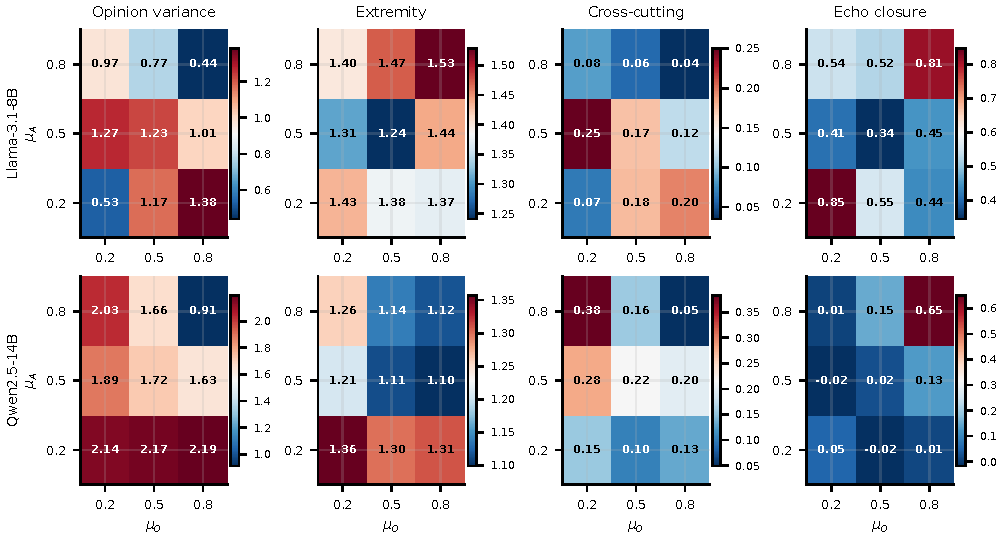
\includegraphics[width=\linewidth]{figures/figS3_full_surfaces.pdf}
\caption*{\small\textbf{Figure S3}\quad Response surfaces for all four polarization measures, in both model families. Cell values are means over seeds.}
\end{figure}

\medskip

\section*{S20\quad The hidden-profile floor in the replication model}
\addcontentsline{toc}{section}{S20\quad The hidden-profile floor in the replication model}
The hidden-profile task discriminates weakly in the primary model and not at all in the replication model, where societies almost never recovered the unshared information. This is why several statistics in Section~S6 are undefined, and why the alignment result in the main text rests on the accuracy measure rather than on hidden-profile solving.
\begin{figure}[H]\centering
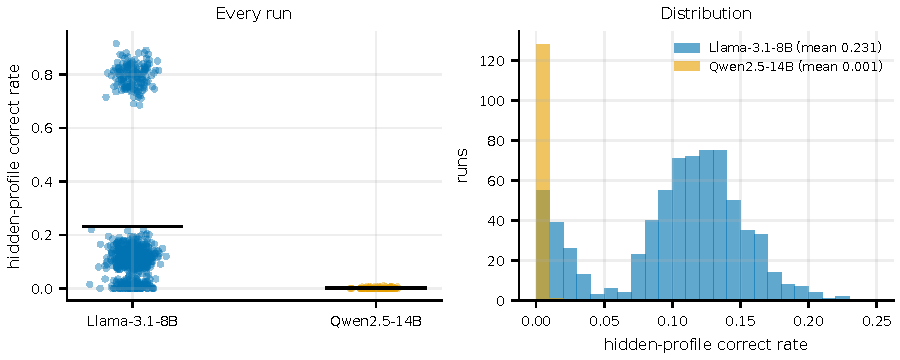
\includegraphics[width=0.86\linewidth]{figures/figS4_hidden_profile_floor.pdf}
\caption*{\small\textbf{Figure S4}\quad Hidden-profile accuracy in every run, by model family. The replication model sits at an absolute floor.}
\end{figure}

\medskip

\section*{S21\quad Validity-principle compliance}
\addcontentsline{toc}{section}{S21\quad Validity-principle compliance}
\begin{longtable}{@{}p{3.2cm}p{10.5cm}@{}}
\toprule
Principle & Implementation \\
\midrule
\endhead
Profile heterogeneity & Trait vectors are sampled per condition from a truncated multivariate normal and validated through the induction gate (Table~S1), not asserted. \\[2pt]
Interaction & Agents exchange content through a recommender-driven feed with follow and unfollow actions; there is no broadcast shortcut. \\[2pt]
Memory & Each agent carries a bounded memory of its recent actions and of any private information it holds. \\[2pt]
Minimal control & Action prompts are open-ended and contain no instruction that presupposes an outcome. The full prompt text is reproduced in Section~S2. \\[2pt]
Unawareness & Agents are never told that they are in an experiment, and the persona prompt forbids self-reference as a language model. \\[2pt]
Realism & One condition is calibrated to published population norms for the same instrument; discussion topics derive from contested policy questions. \\[2pt]
\bottomrule
\end{longtable}

\end{document}
